\subsection{Comparison of Raw Spectra}

In this section, raw data spectra without event selection are compared to PYTHIA8 generator in order to study the possible noise, contribution of fake jets and fake tracks, and other possible experimental backgrounds. The results are shown in the figures below.

%The spike in the LEP1 and LEP2 pt spectra near 45 GeV is produced by the particles that took the full beam energy in the transverse plane. The beam energy is 92 GeV so in a two particle configuration each particle will take half of the total energy to conserve various kinematics. 

\subsection{Raw data}
\begin{figure}[H]
\centering
\subfloat{\label{sfig:a}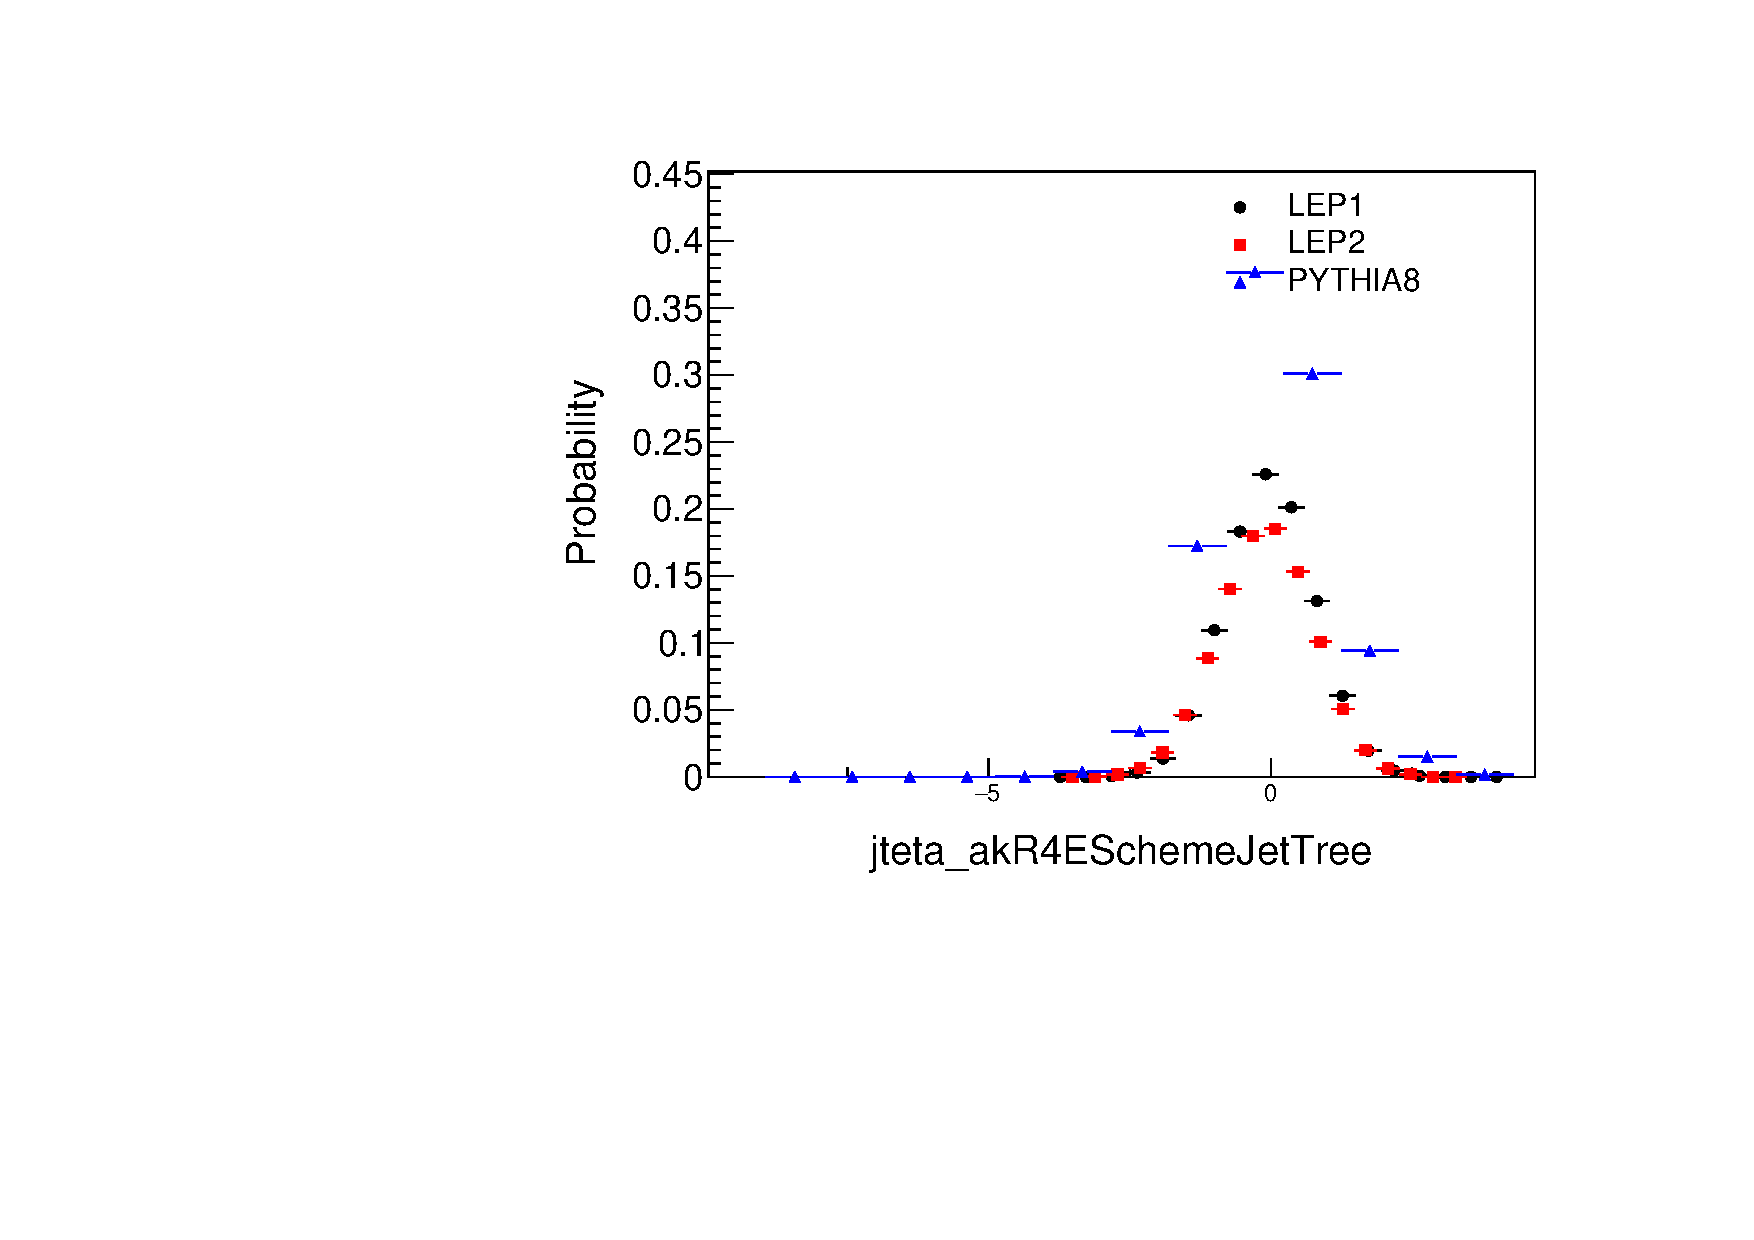
\includegraphics[width=.25\textwidth]{images/DQC/NoCut/jteta_akR4ESchemeJetTree.pdf}}\hfill
\subfloat{\label{sfig:b}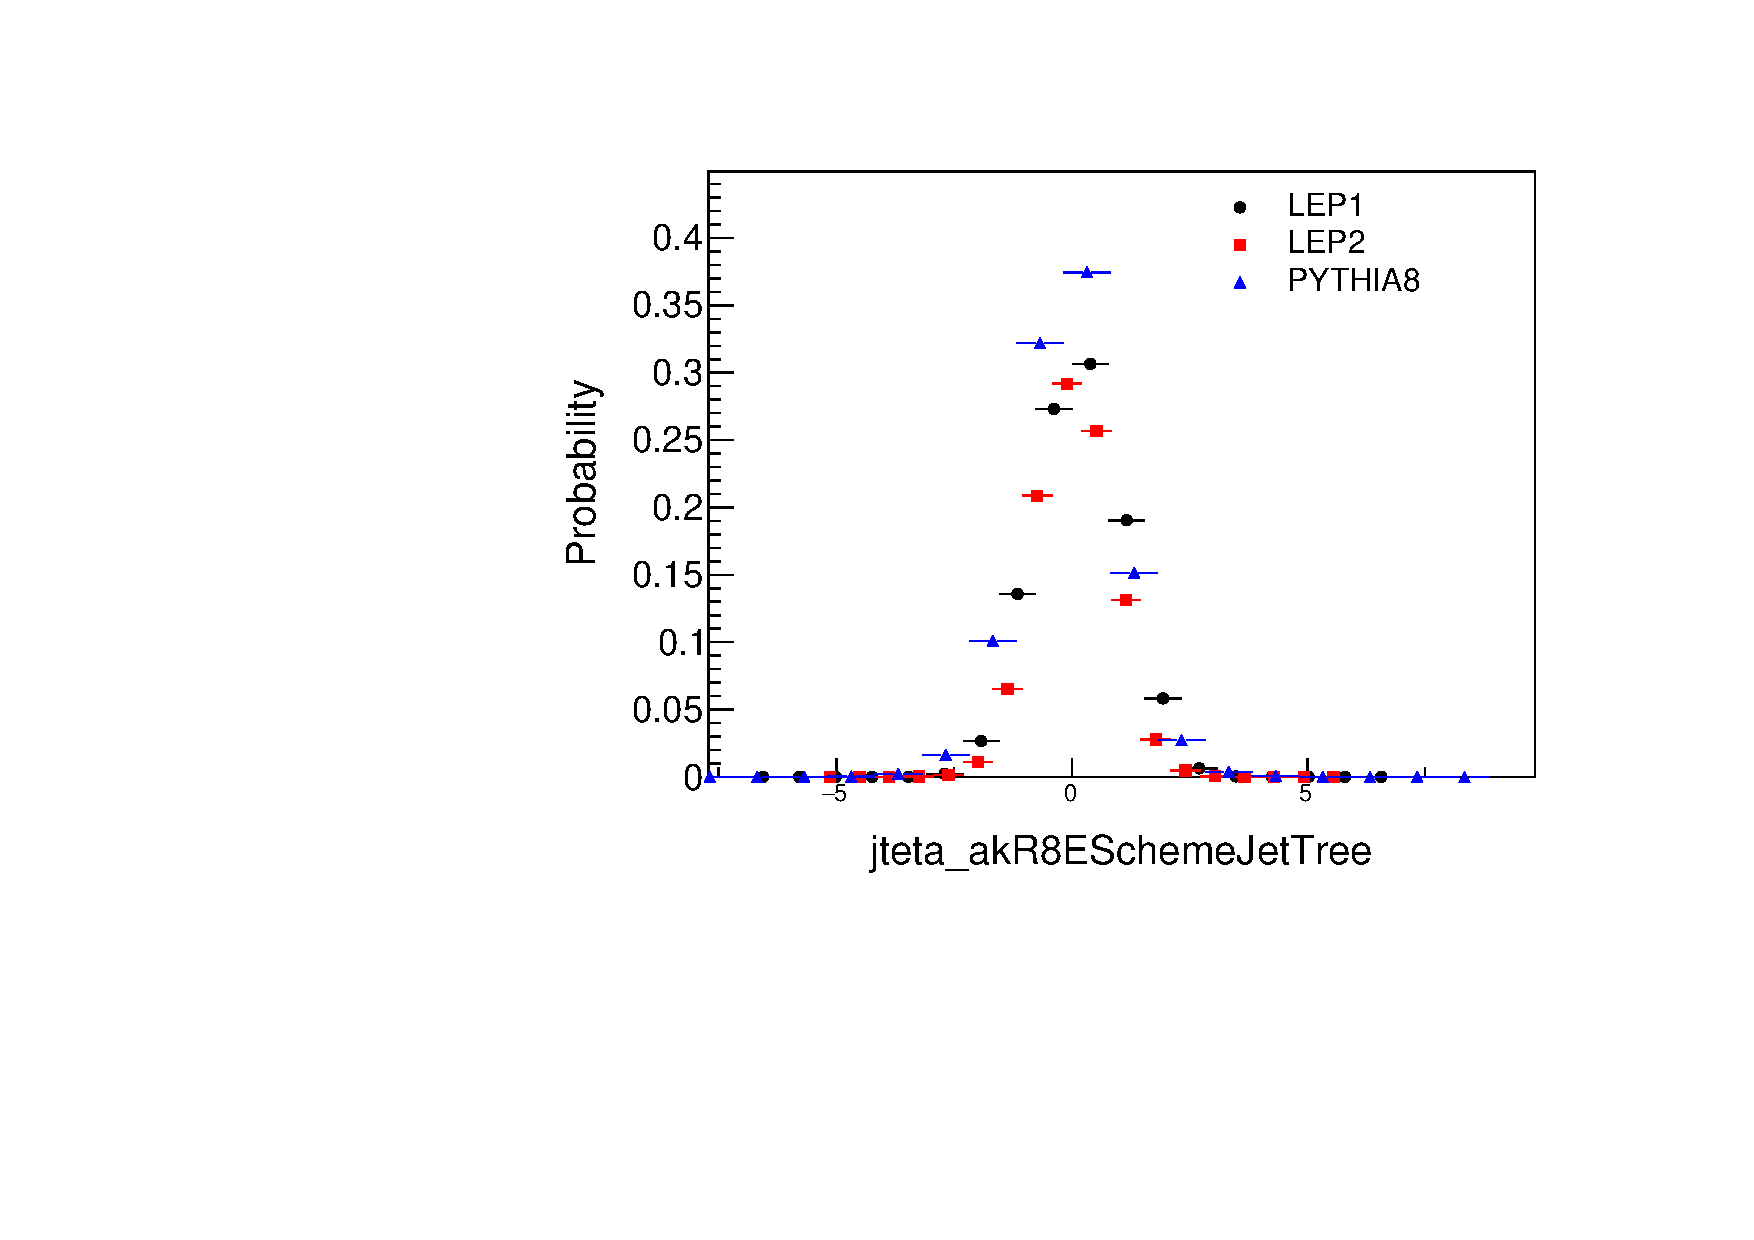
\includegraphics[width=.25\textwidth]{images/DQC/NoCut/jteta_akR8ESchemeJetTree.pdf}}\hfill
\subfloat{\label{sfig:c}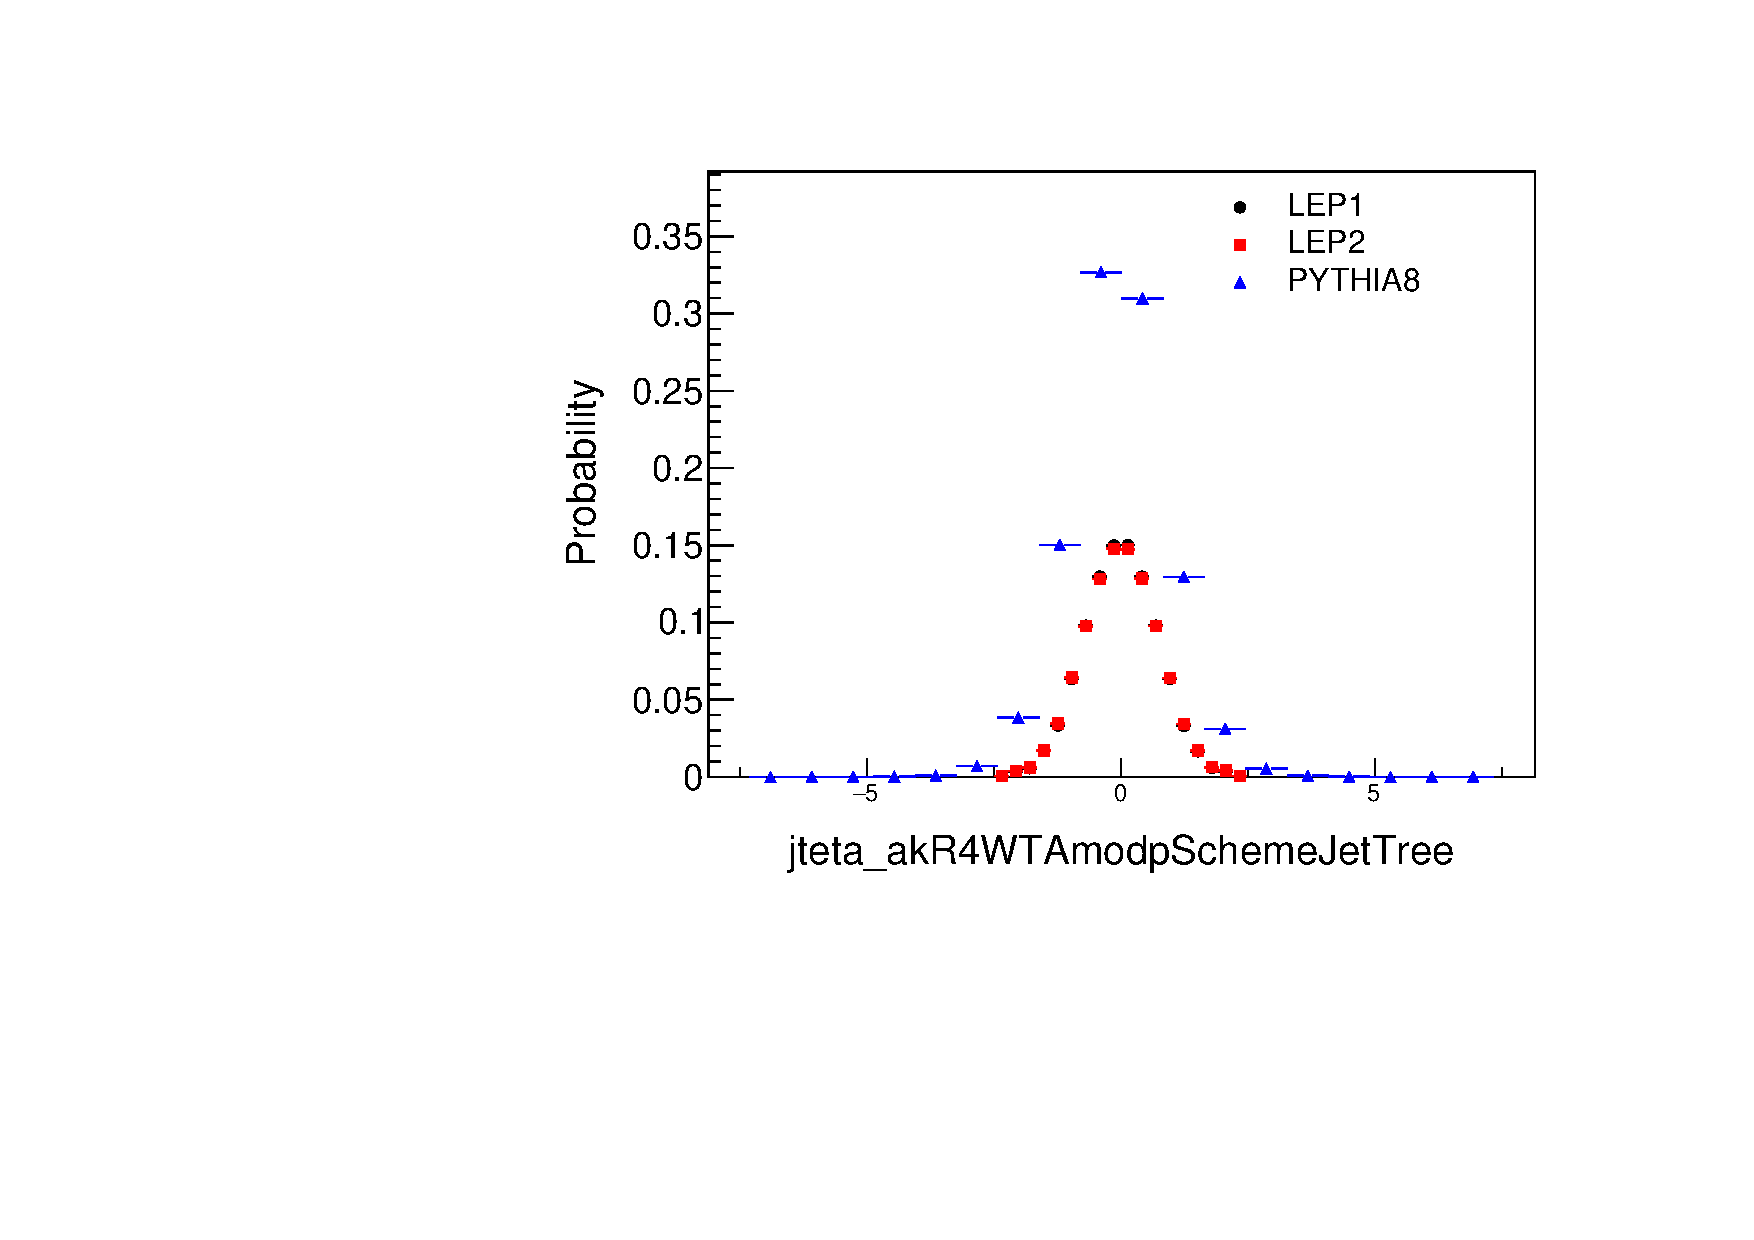
\includegraphics[width=.25\textwidth]{images/DQC/NoCut/jteta_akR4WTAmodpSchemeJetTree.pdf}}\hfill
\subfloat{\label{sfig:d}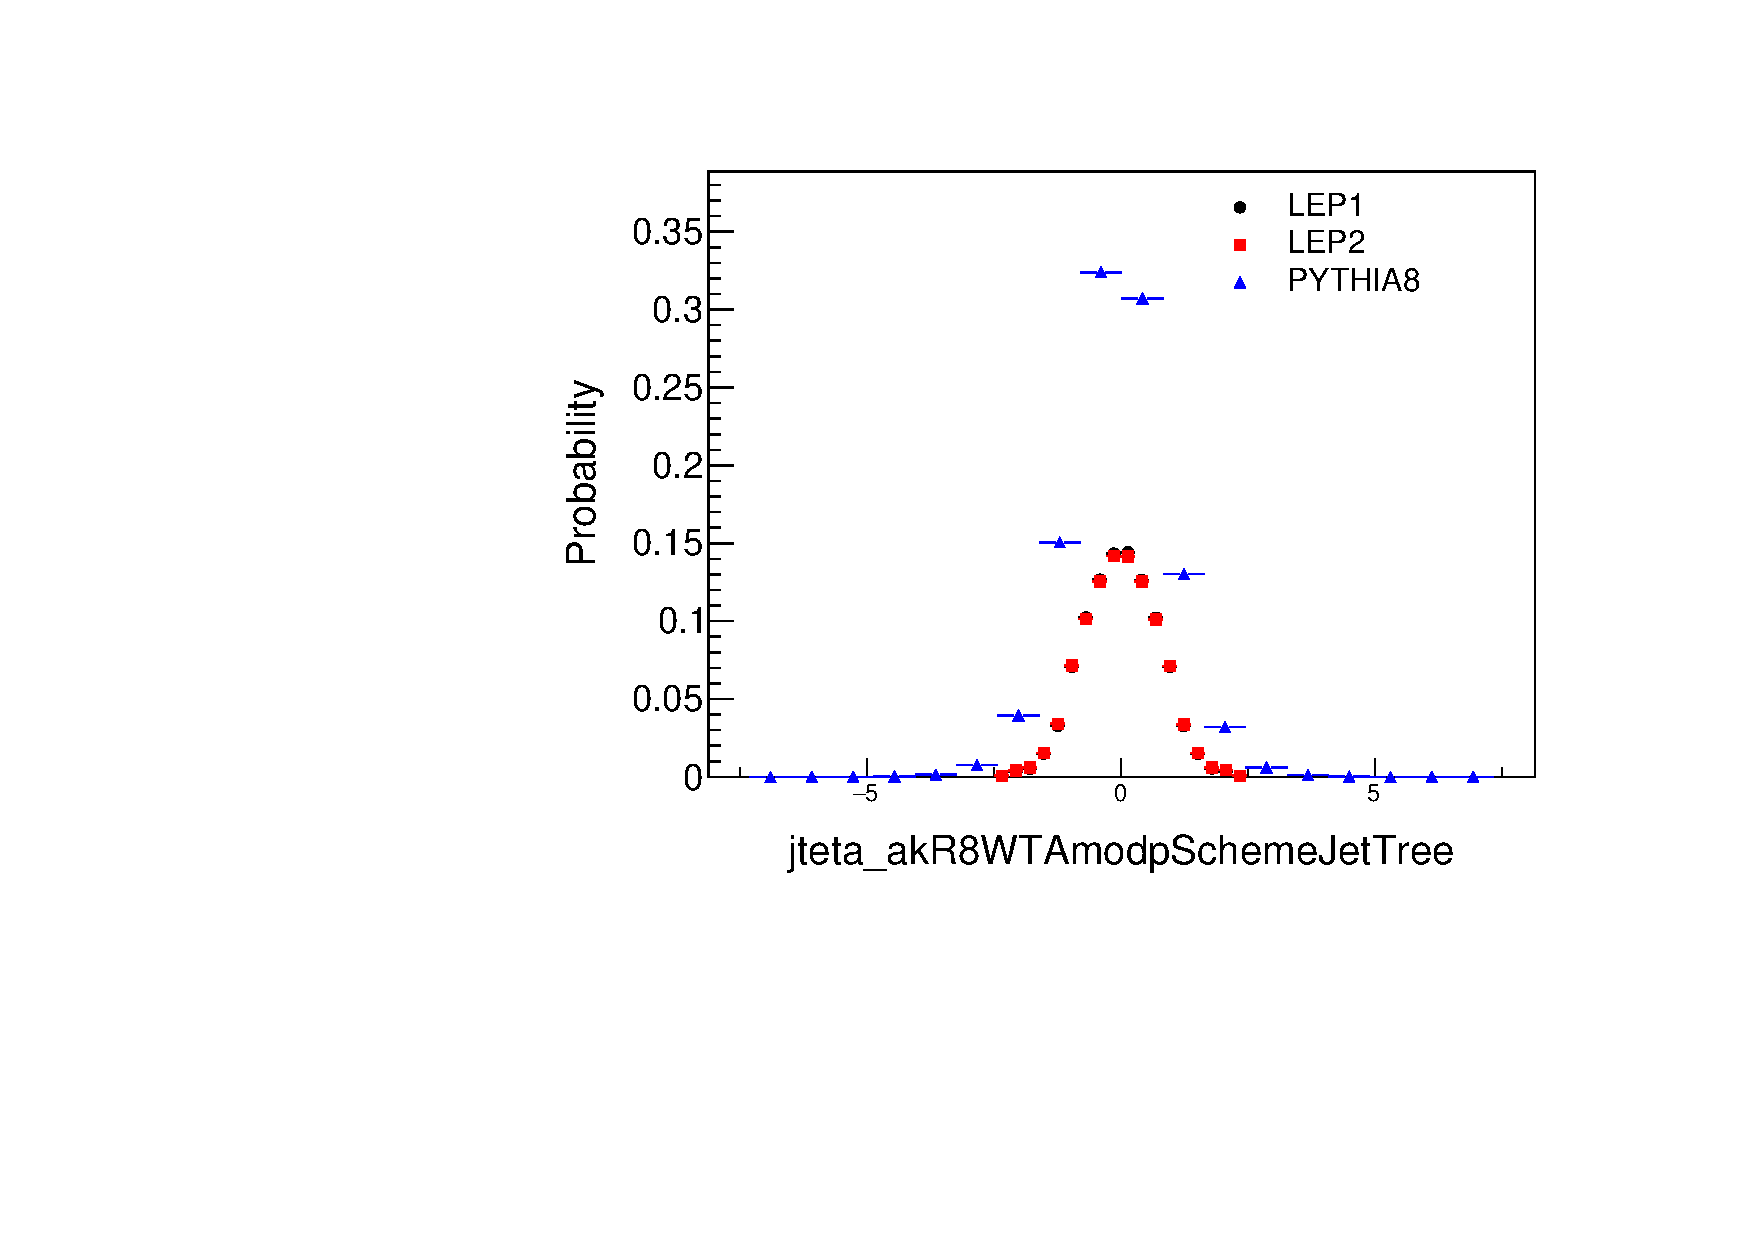
\includegraphics[width=.25\textwidth]{images/DQC/NoCut/jteta_akR8WTAmodpSchemeJetTree.pdf}}\hfill %row end
\subfloat{\label{sfig:e}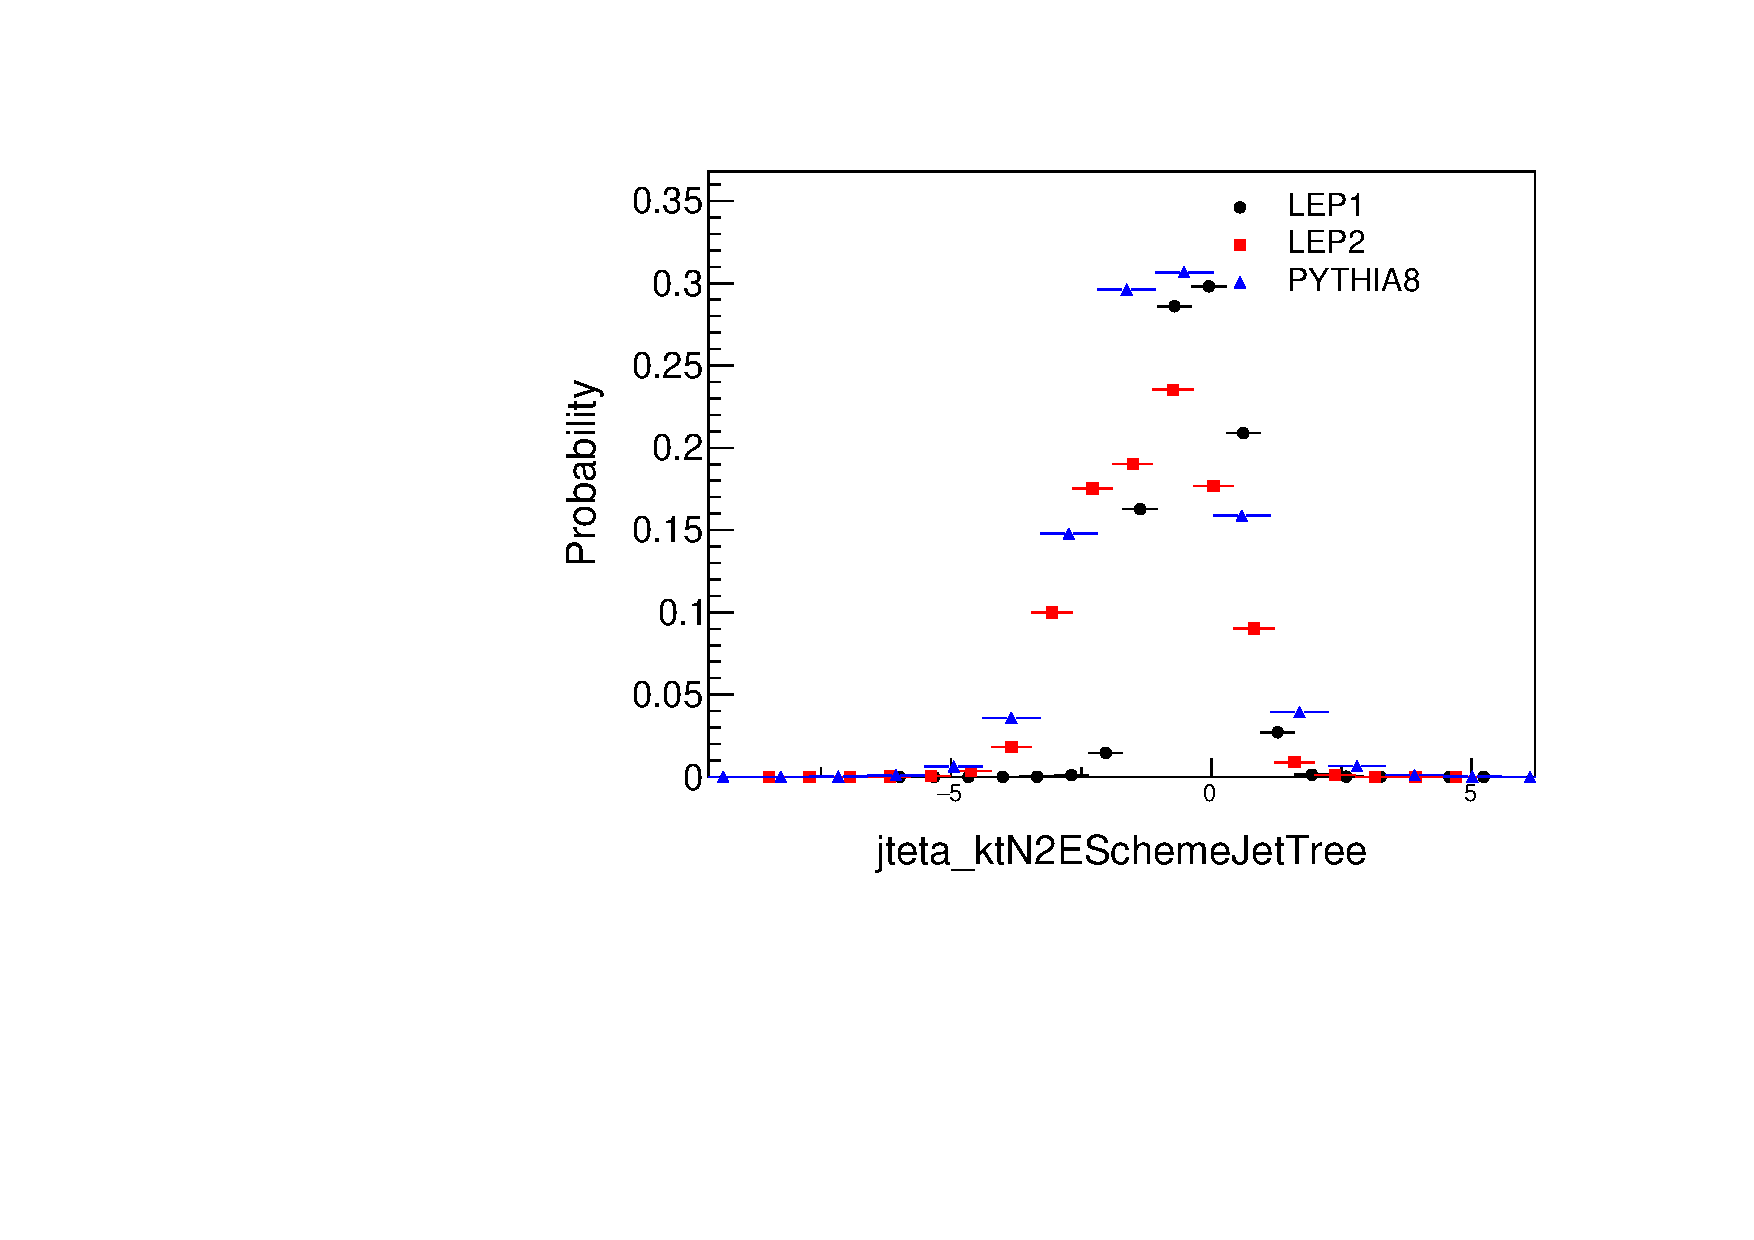
\includegraphics[width=.25\textwidth]{images/DQC/NoCut/jteta_ktN2ESchemeJetTree.pdf}}\hfill
\subfloat{\label{sfig:f}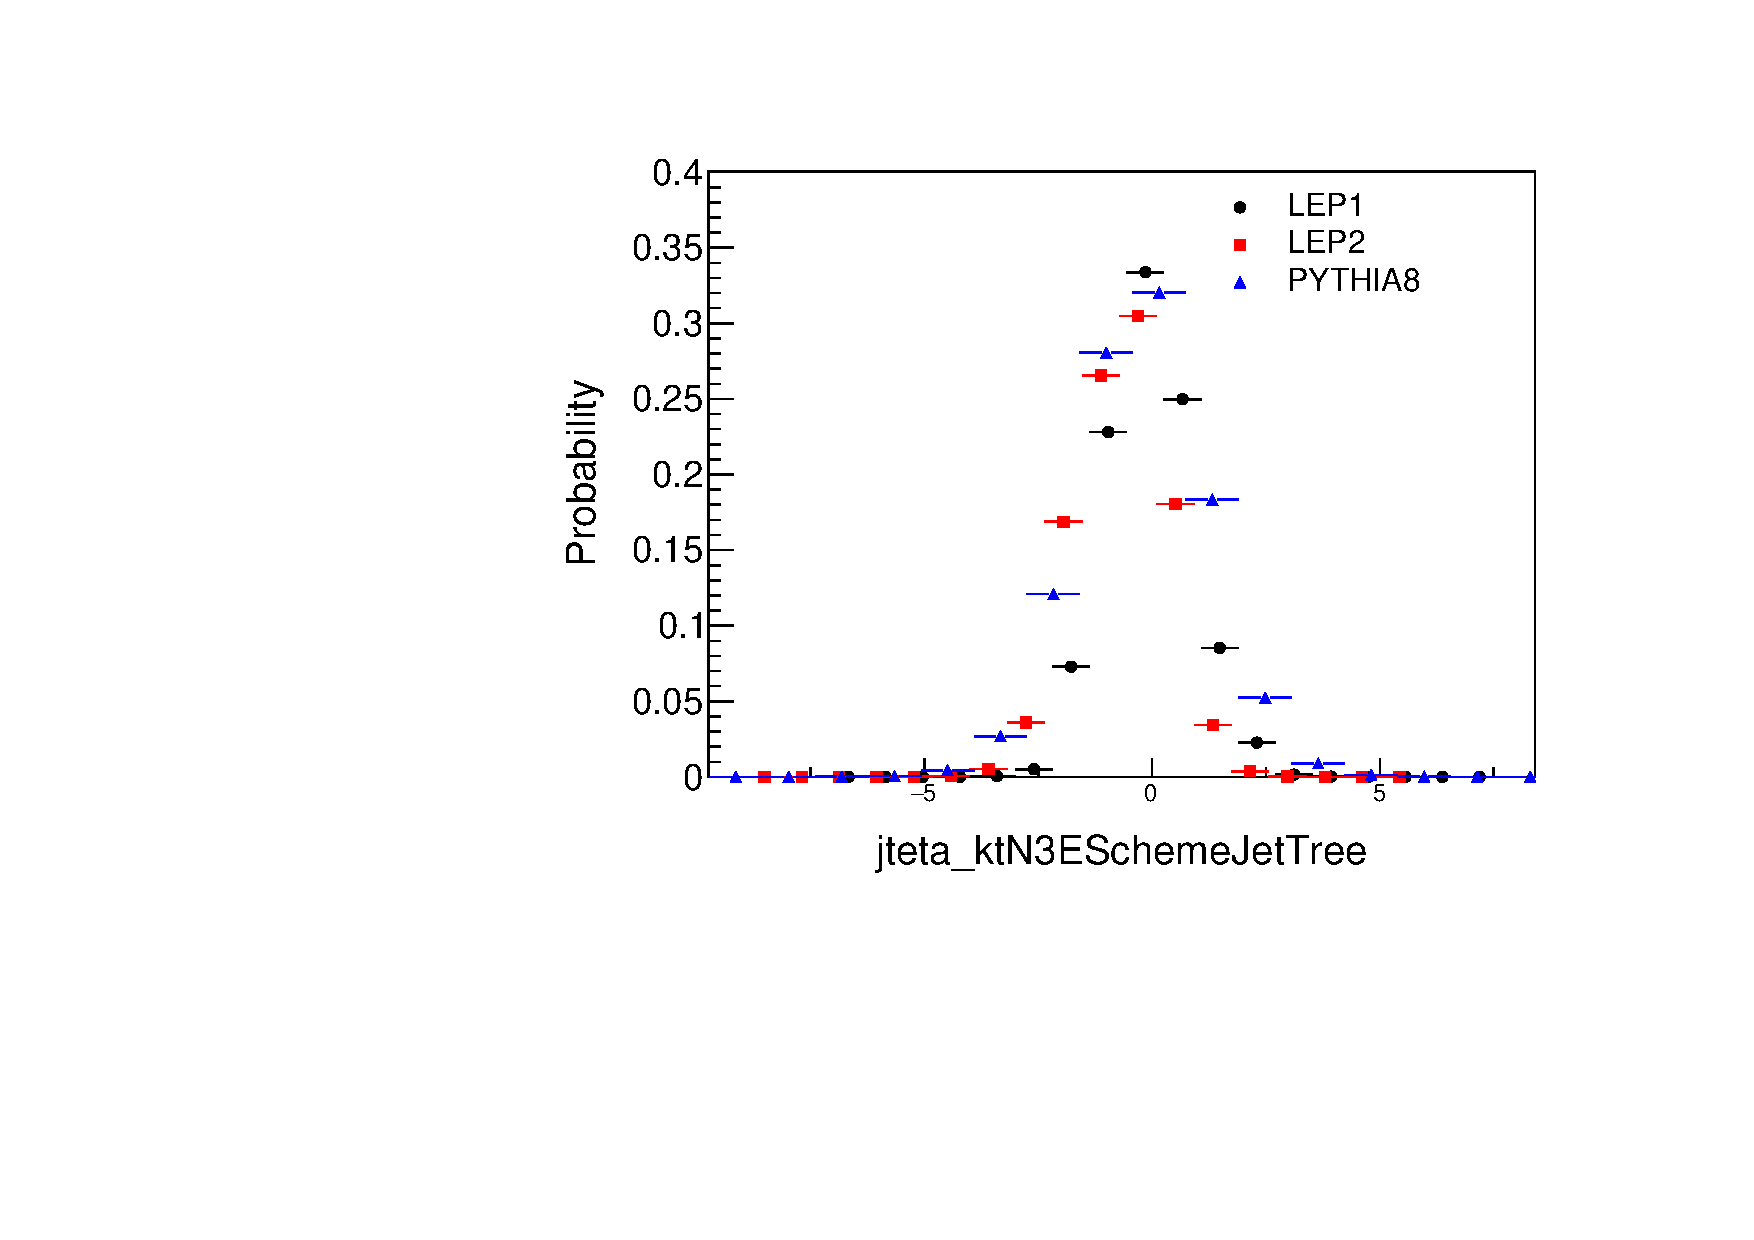
\includegraphics[width=.25\textwidth]{images/DQC/NoCut/jteta_ktN3ESchemeJetTree.pdf}}\hfill
\subfloat{\label{sfig:g}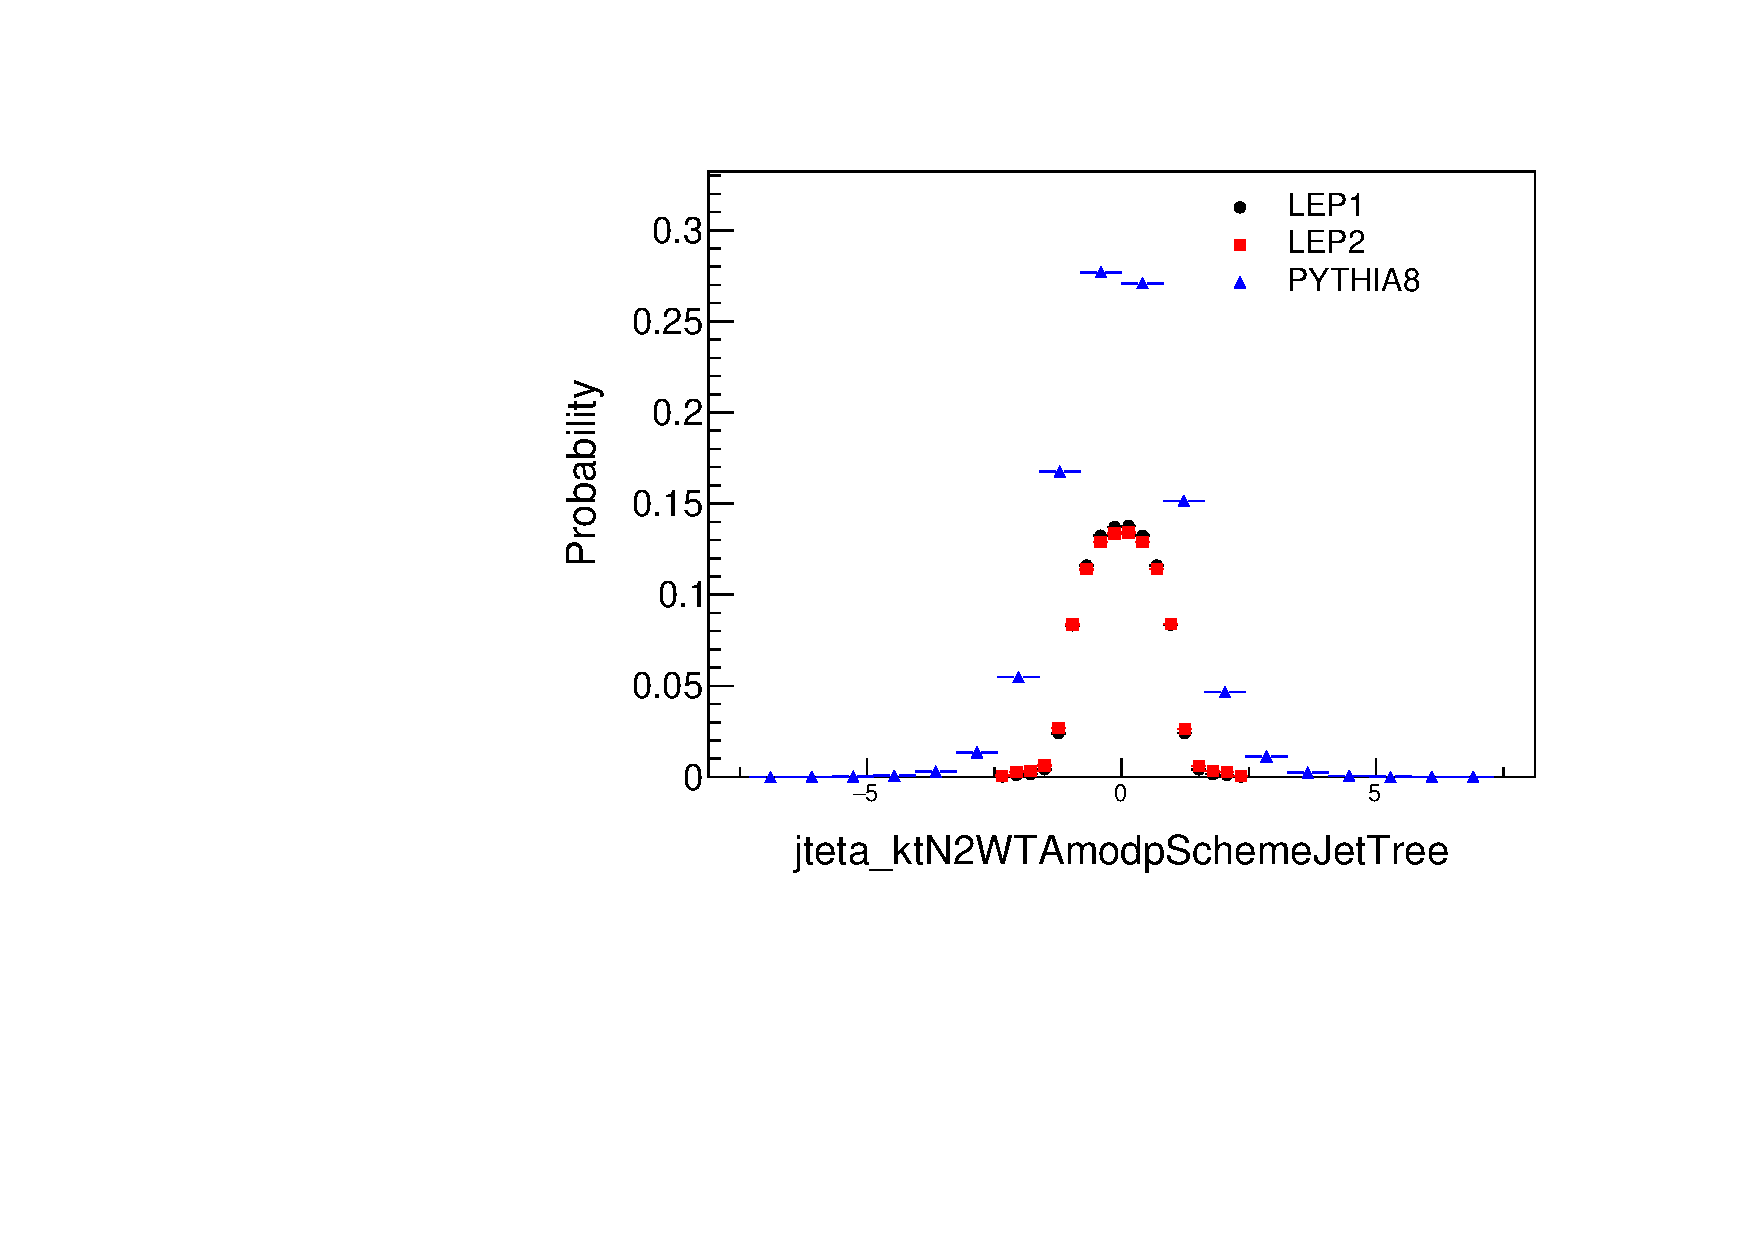
\includegraphics[width=.25\textwidth]{images/DQC/NoCut/jteta_ktN2WTAmodpSchemeJetTree.pdf}}\hfill
\subfloat{\label{sfig:h}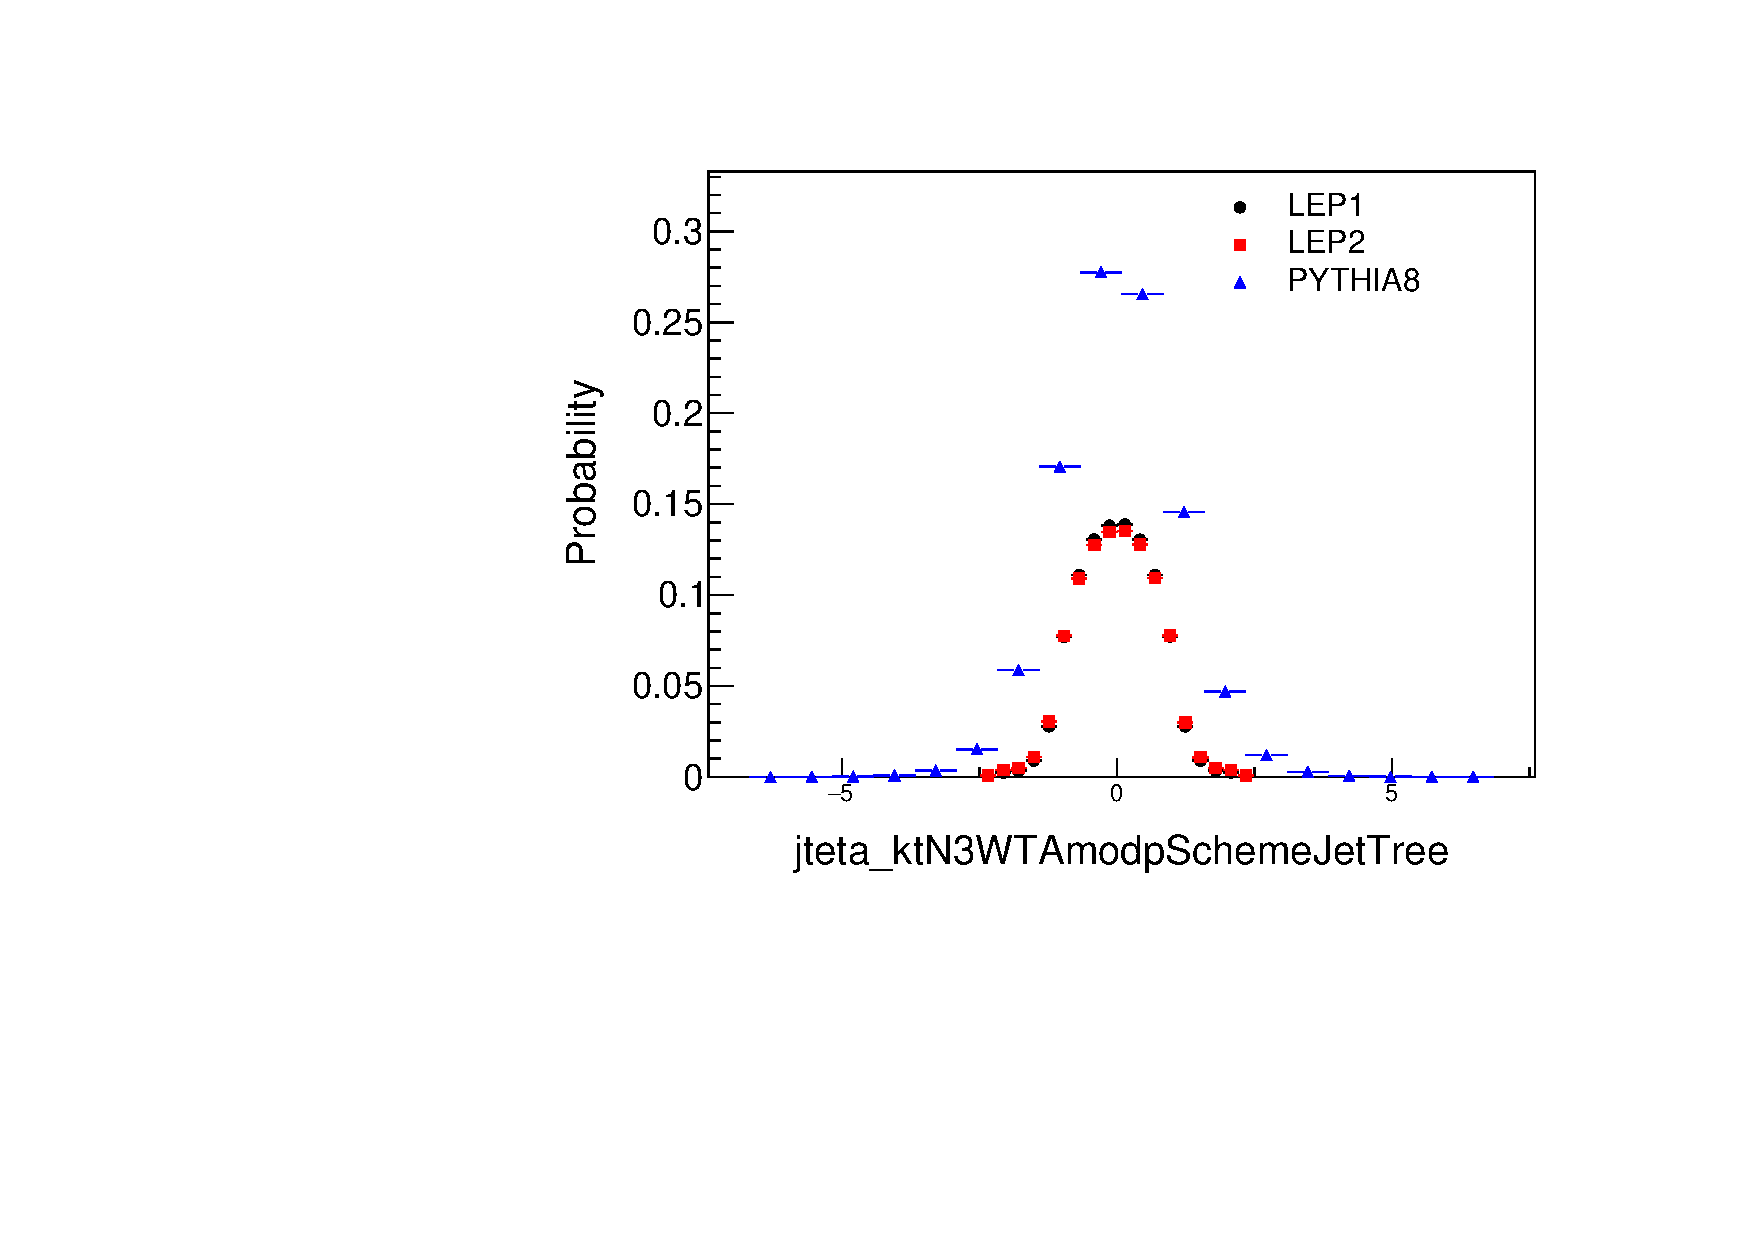
\includegraphics[width=.25\textwidth]{images/DQC/NoCut/jteta_ktN3WTAmodpSchemeJetTree.pdf}}\hfill
\caption{Raw Data: LEP1, LEP2, Pythia8 no cuts. Jet $\eta$ distributions. Top row: anti-$k_t$, left to right: $R=0.4$, $E$ scheme; $R=0.8$, $E$ scheme; $R=0.4$, WTA mod p scheme; $R=0.8$, WTA mod p scheme. Bottom row: $k_t$, left to right: $N=2$, $E$ scheme; $N=3$, $E$ scheme; $N=2$, WTA mod p scheme; $N=3$; WTA mod p scheme.}  
\end{figure}

\begin{figure}[H]
\centering
\subfloat{\label{sfig:a}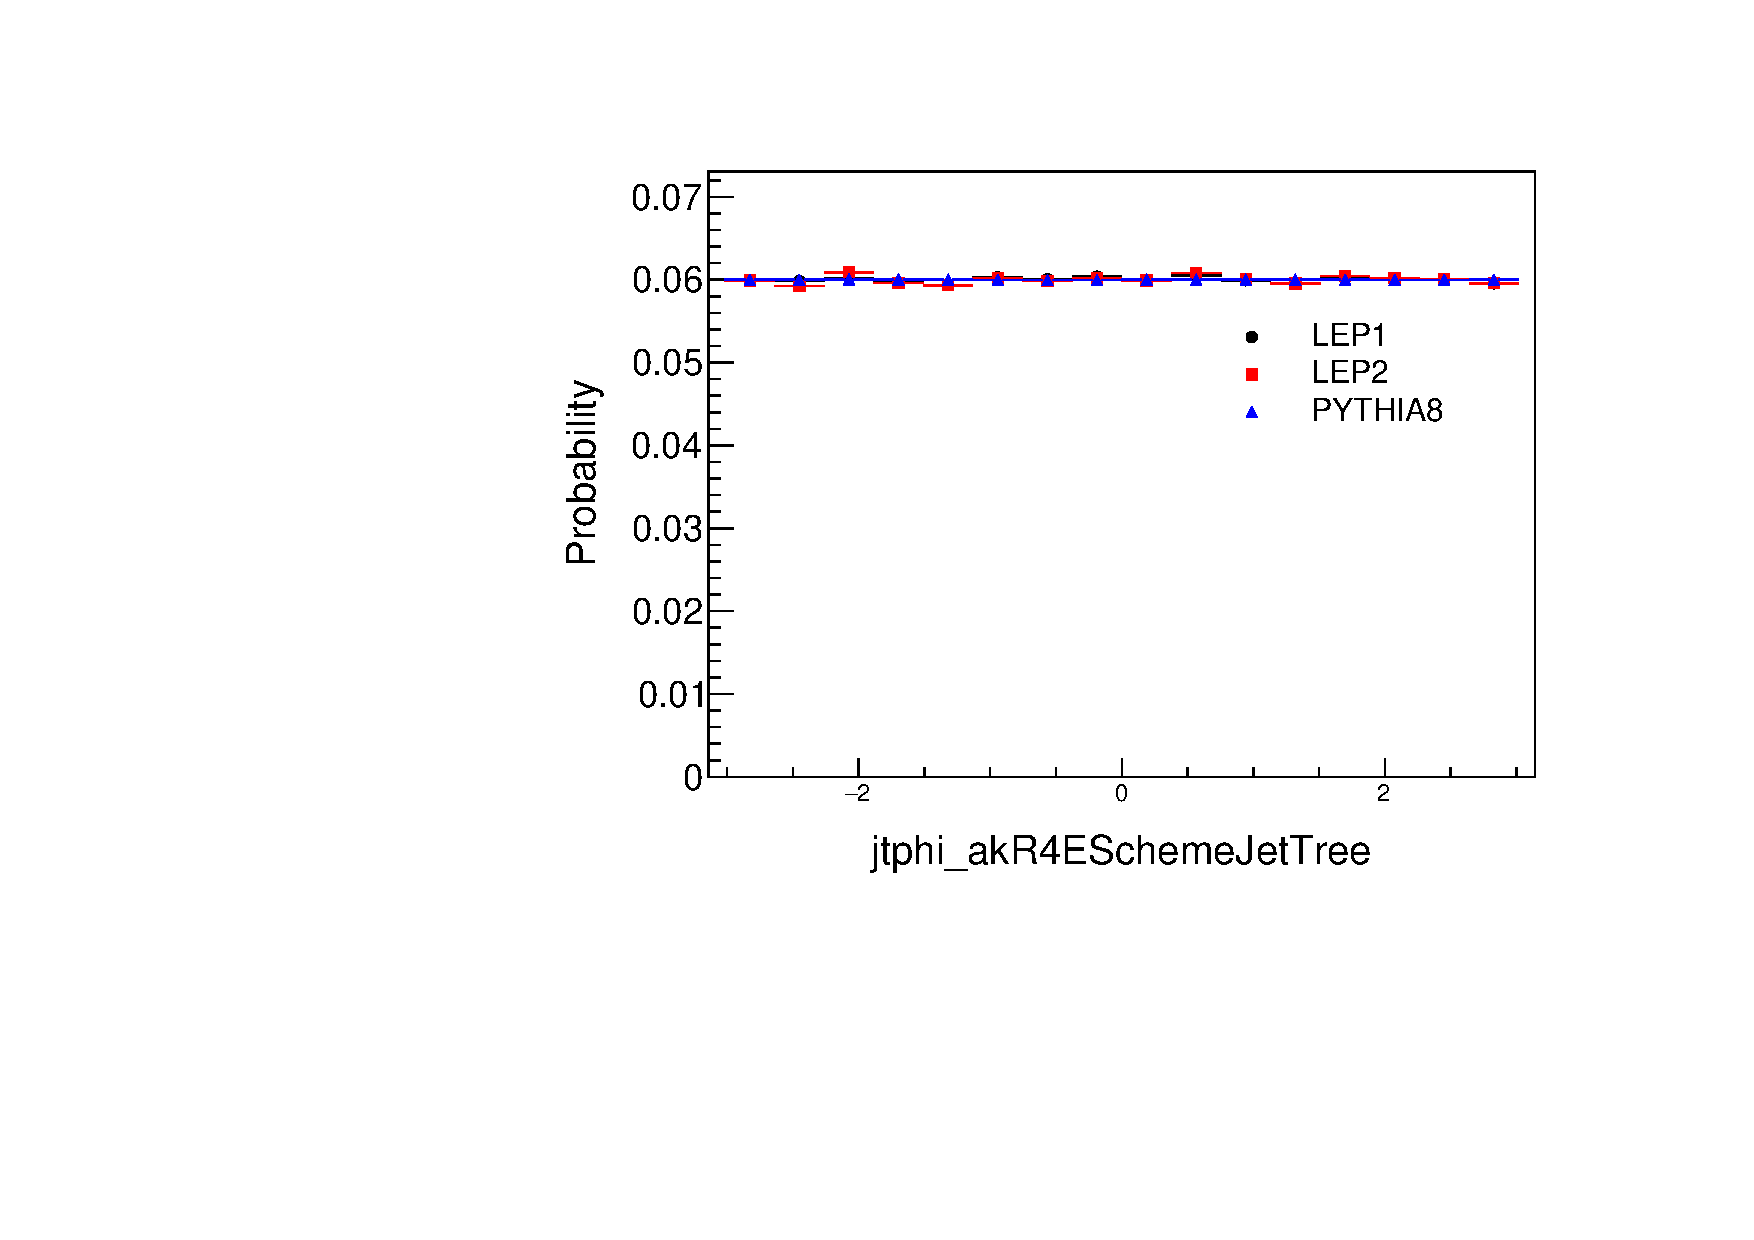
\includegraphics[width=.25\textwidth]{images/DQC/NoCut/jtphi_akR4ESchemeJetTree.pdf}}\hfill
\subfloat{\label{sfig:b}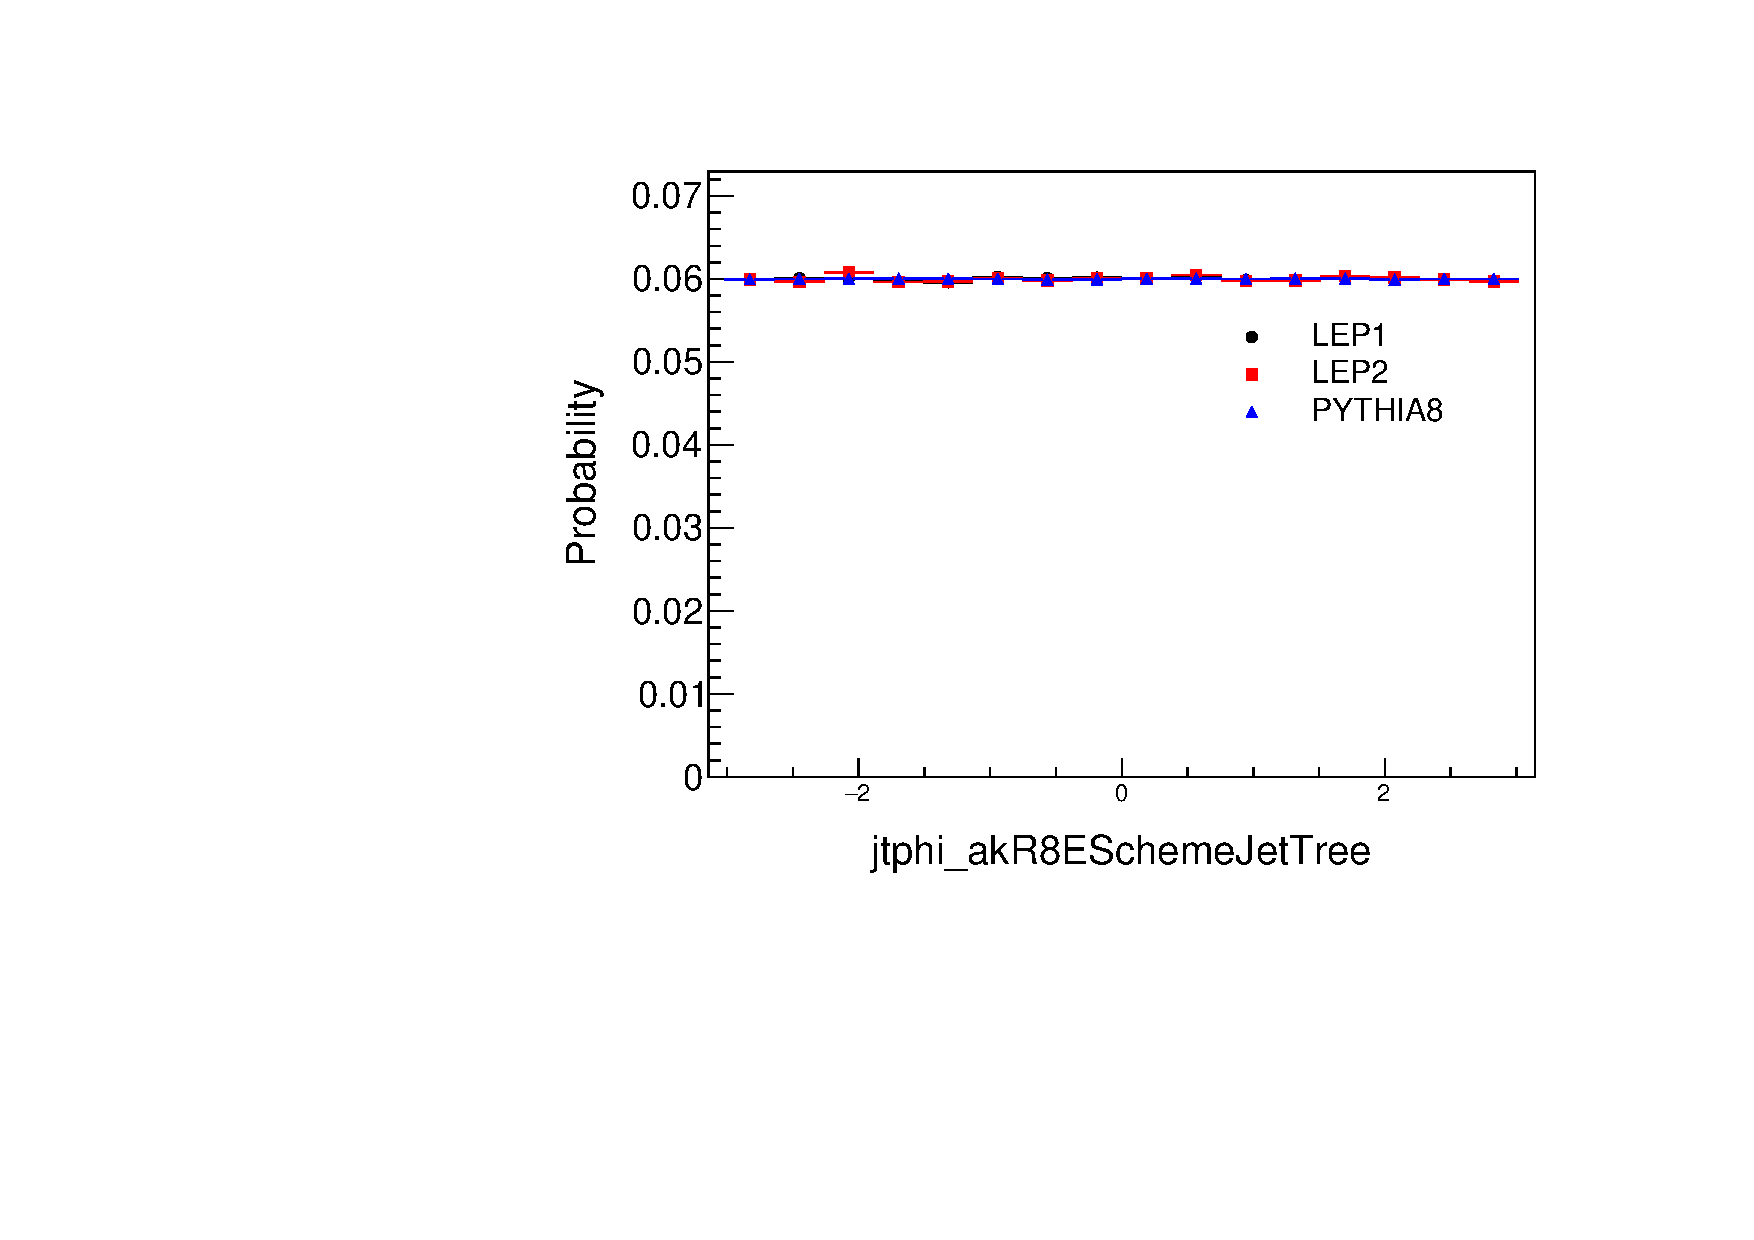
\includegraphics[width=.25\textwidth]{images/DQC/NoCut/jtphi_akR8ESchemeJetTree.pdf}}\hfill
\subfloat{\label{sfig:c}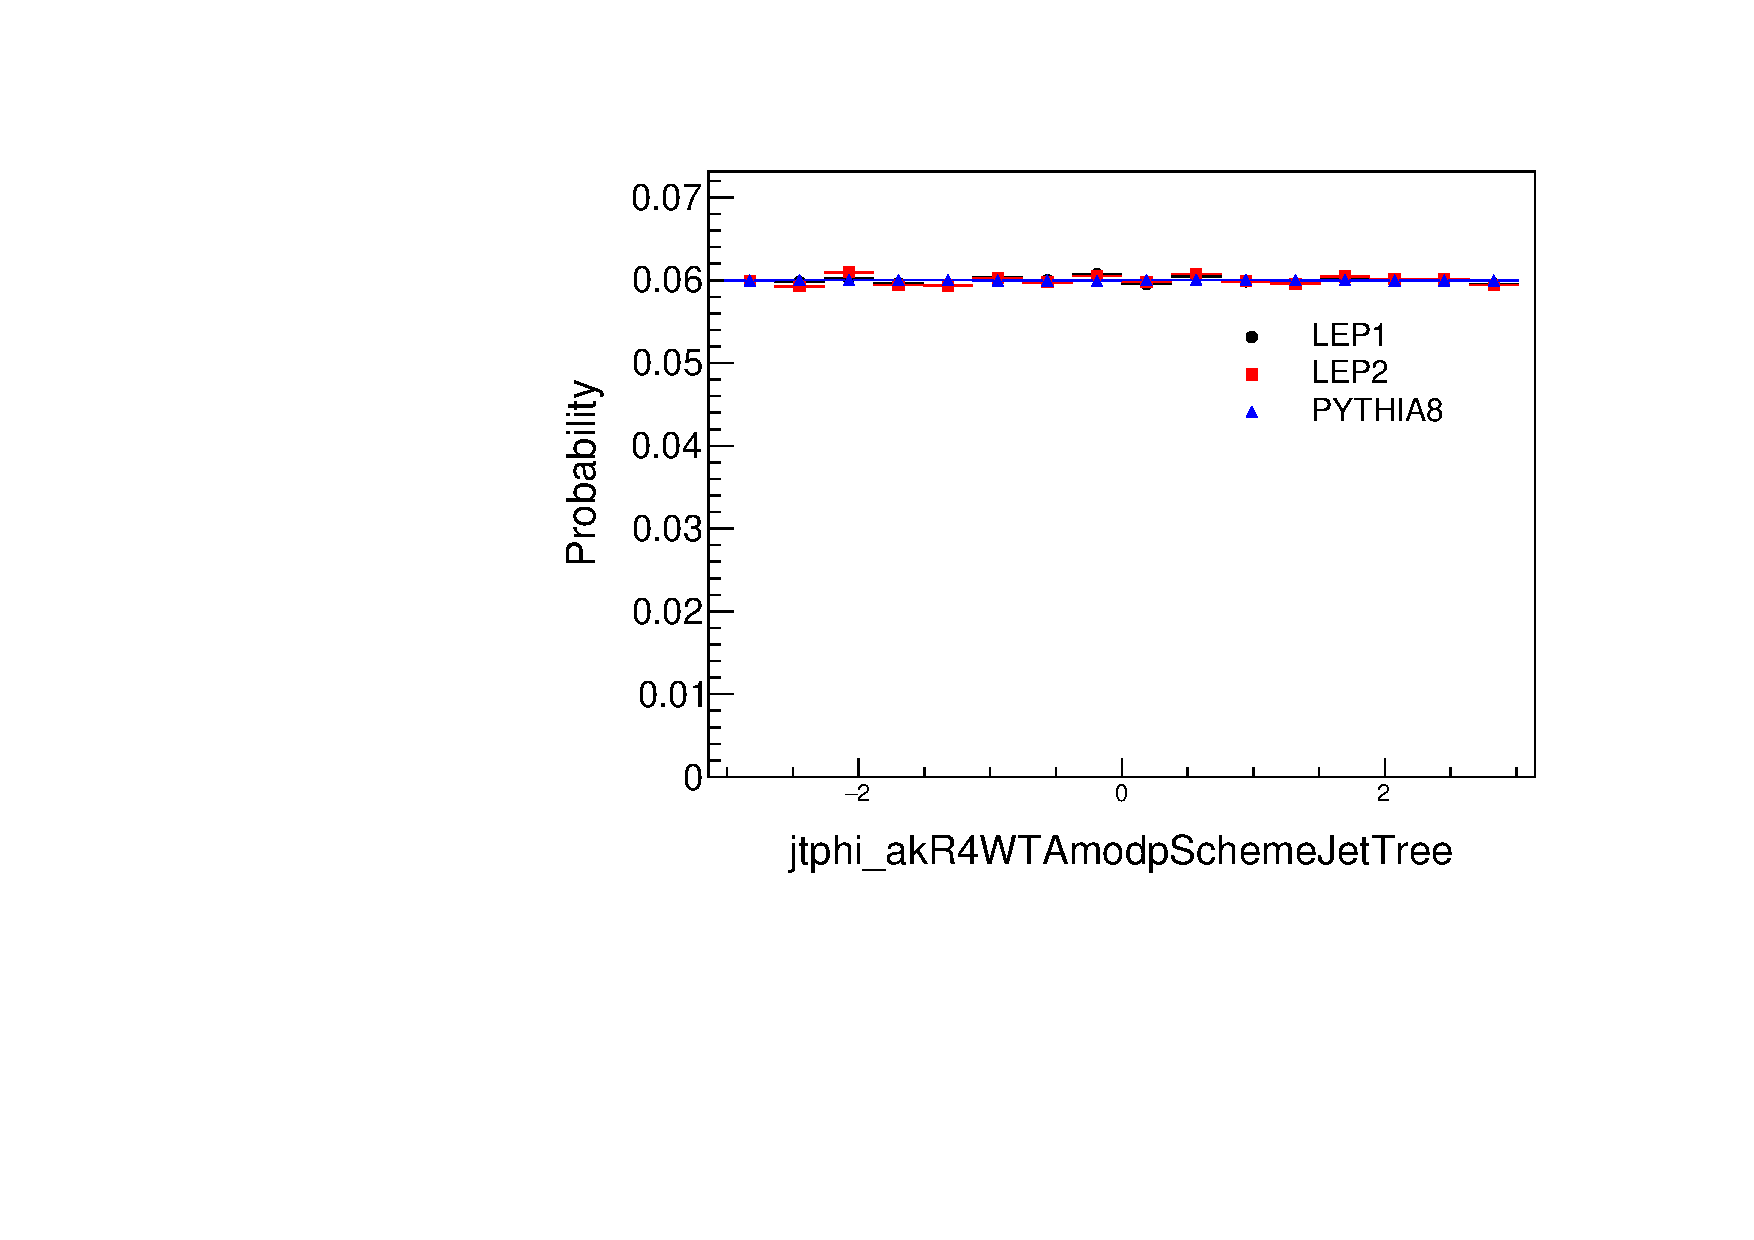
\includegraphics[width=.25\textwidth]{images/DQC/NoCut/jtphi_akR4WTAmodpSchemeJetTree.pdf}}\hfill
\subfloat{\label{sfig:d}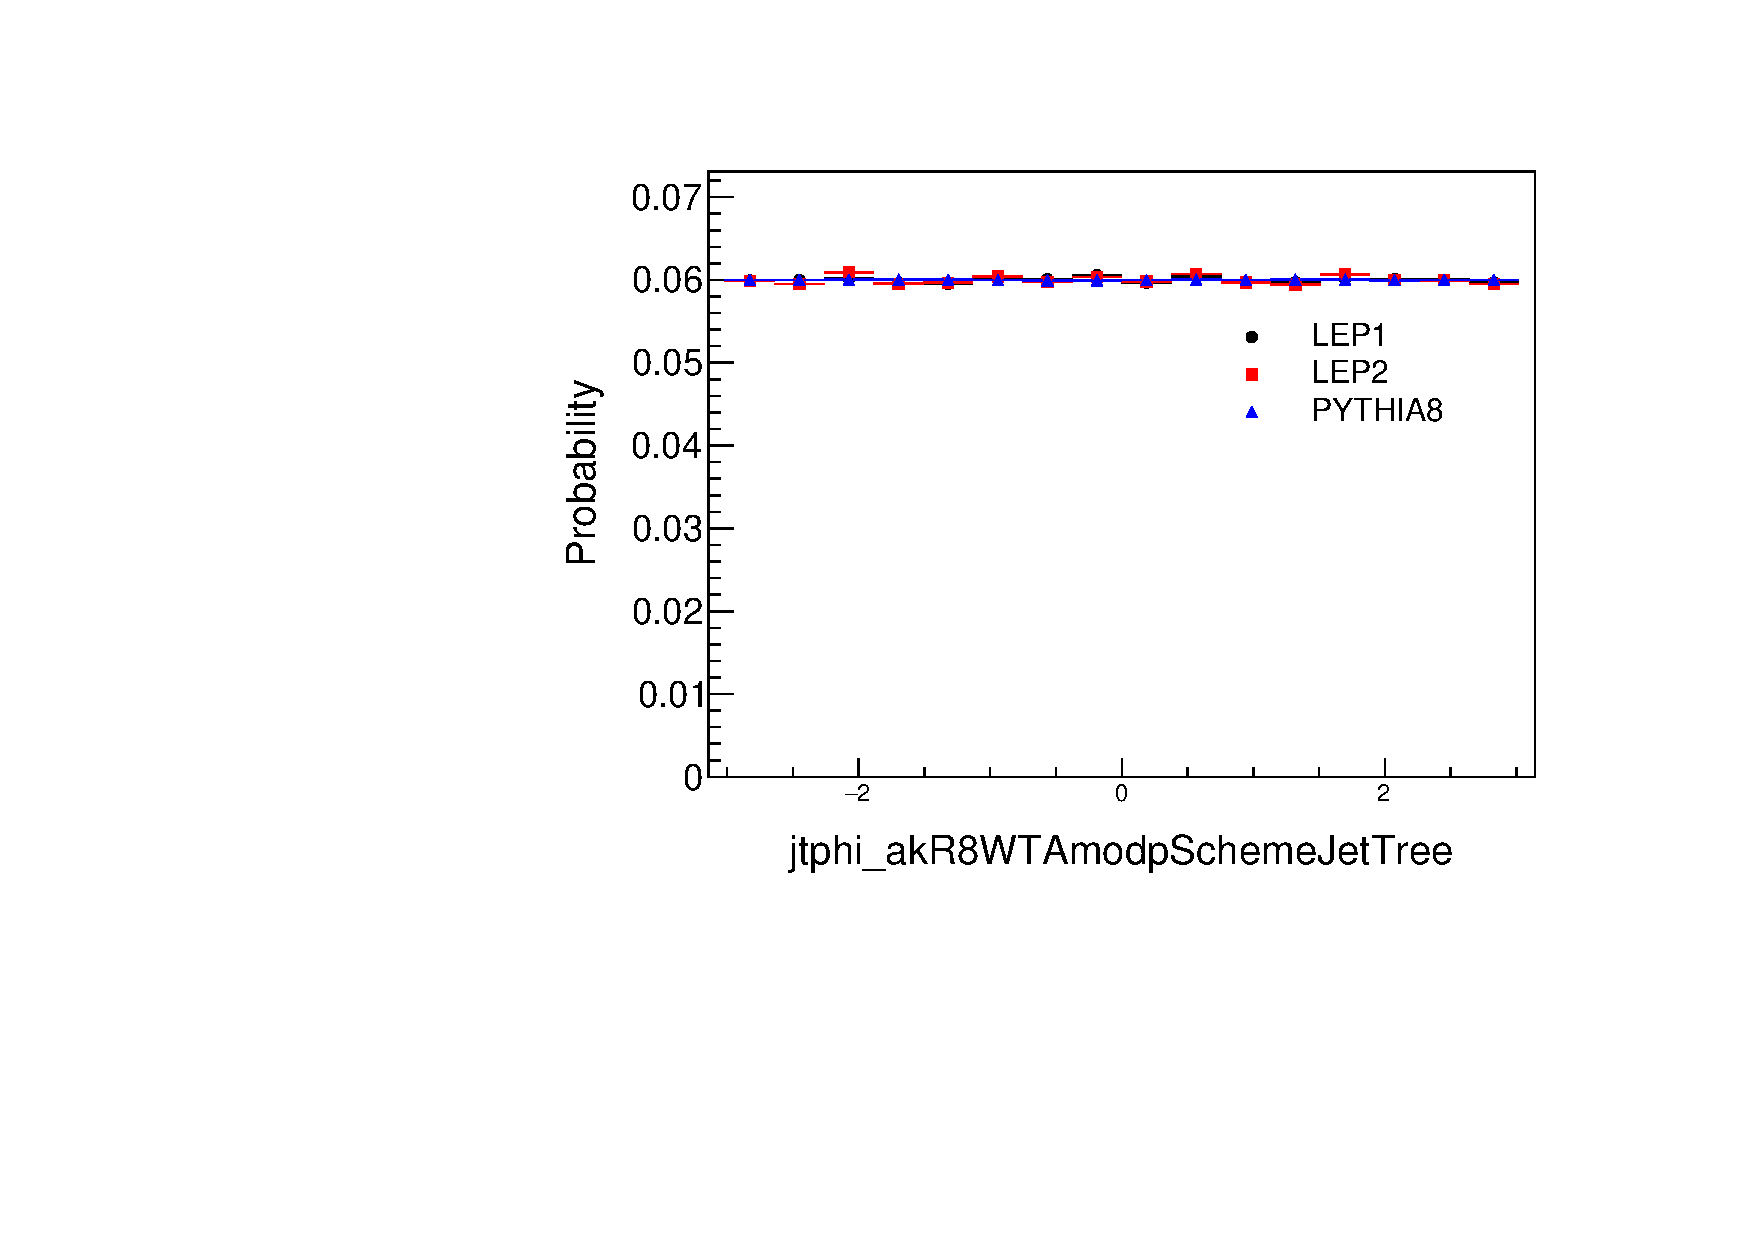
\includegraphics[width=.25\textwidth]{images/DQC/NoCut/jtphi_akR8WTAmodpSchemeJetTree.pdf}}\hfill %row end
\subfloat{\label{sfig:e}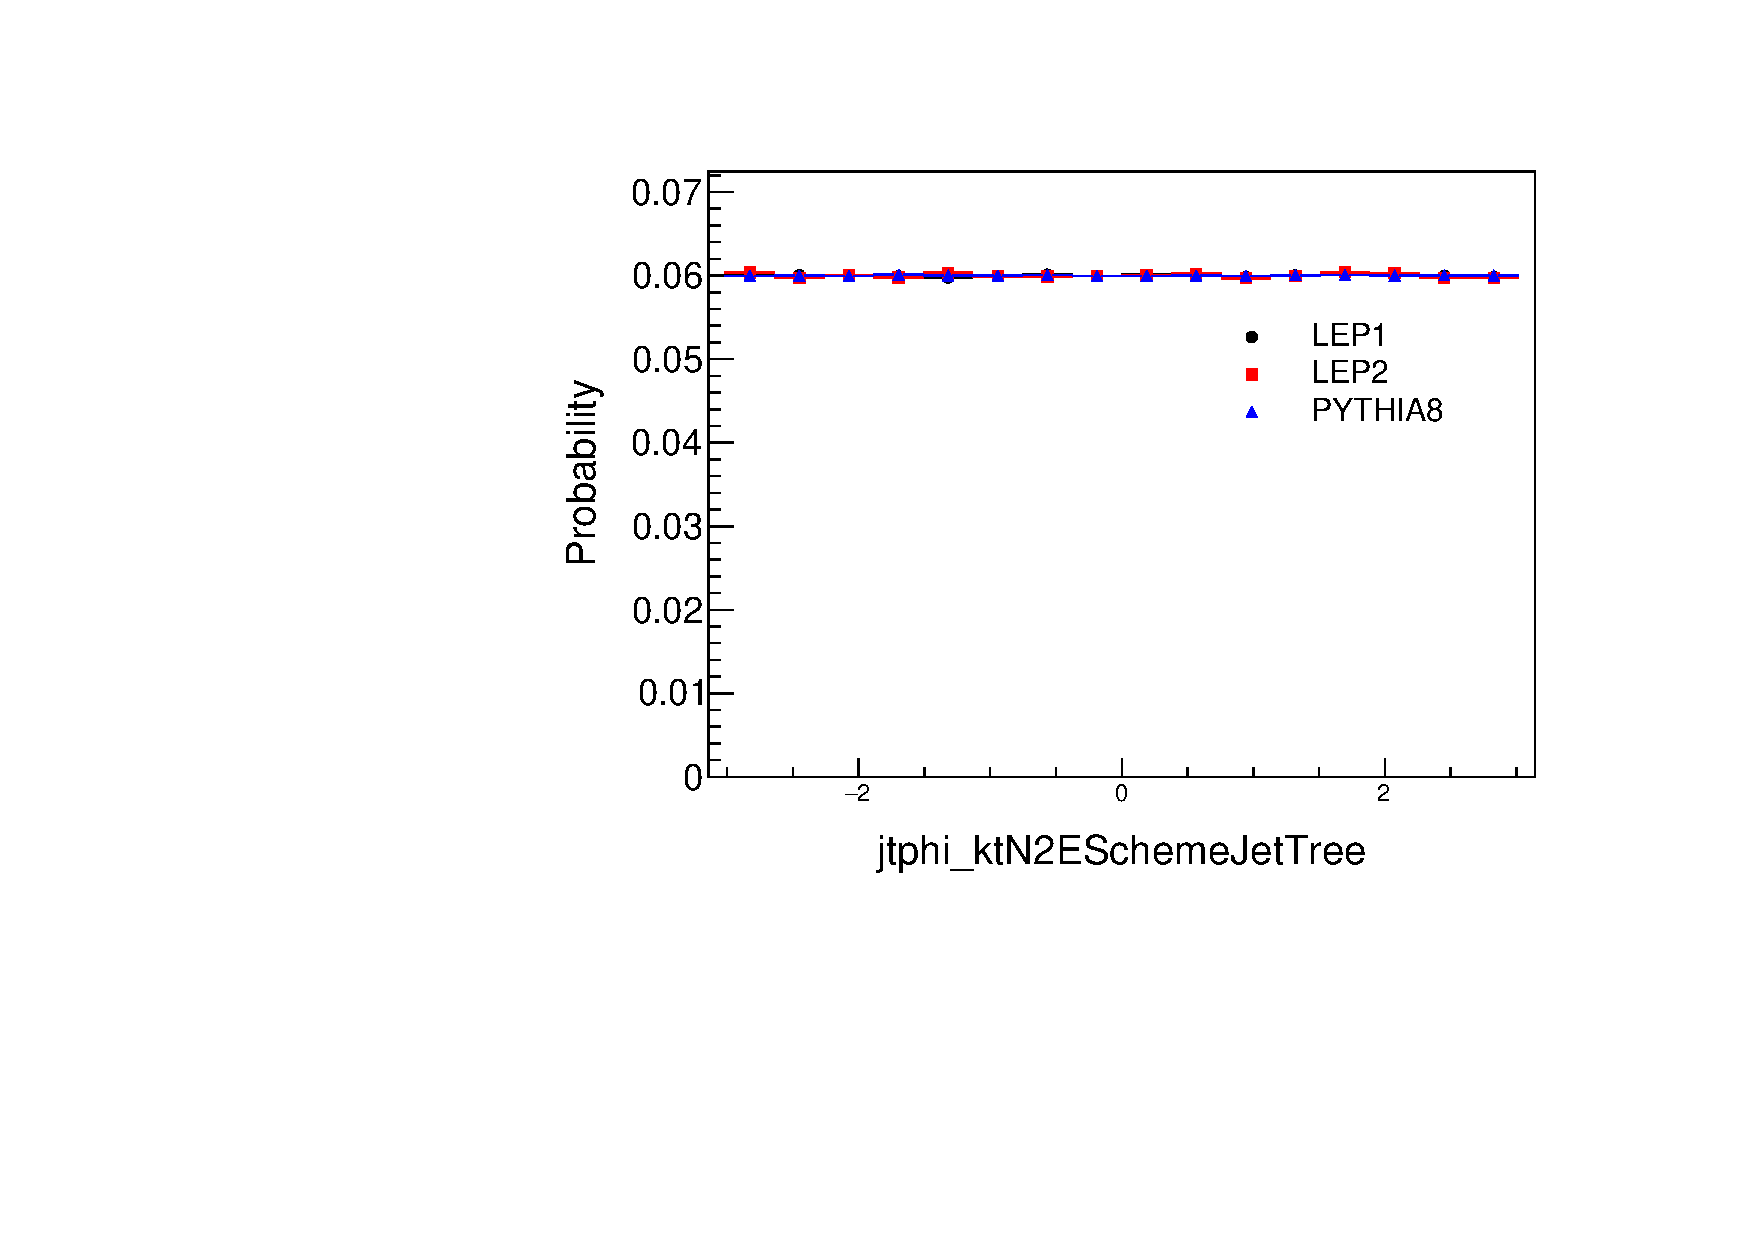
\includegraphics[width=.25\textwidth]{images/DQC/NoCut/jtphi_ktN2ESchemeJetTree.pdf}}\hfill
\subfloat{\label{sfig:f}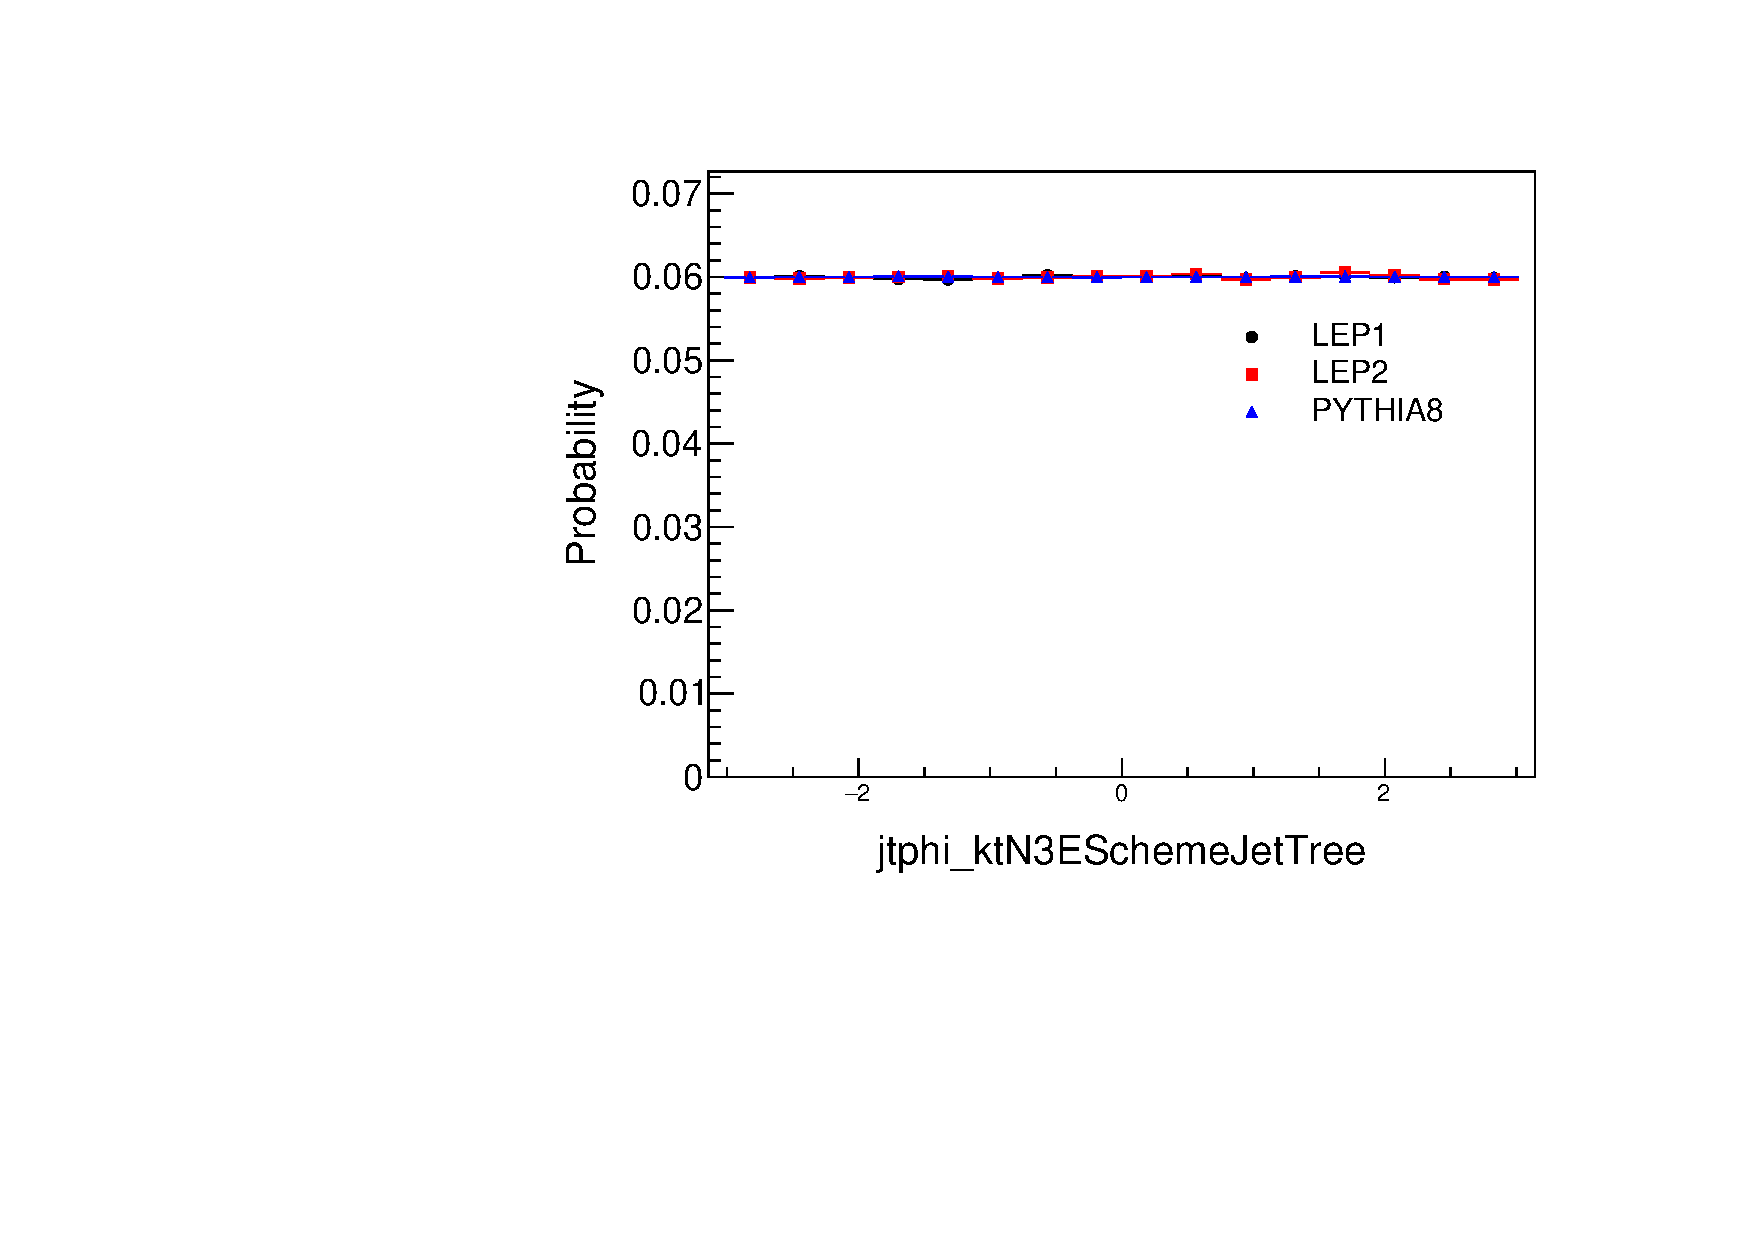
\includegraphics[width=.25\textwidth]{images/DQC/NoCut/jtphi_ktN3ESchemeJetTree.pdf}}\hfill
\subfloat{\label{sfig:g}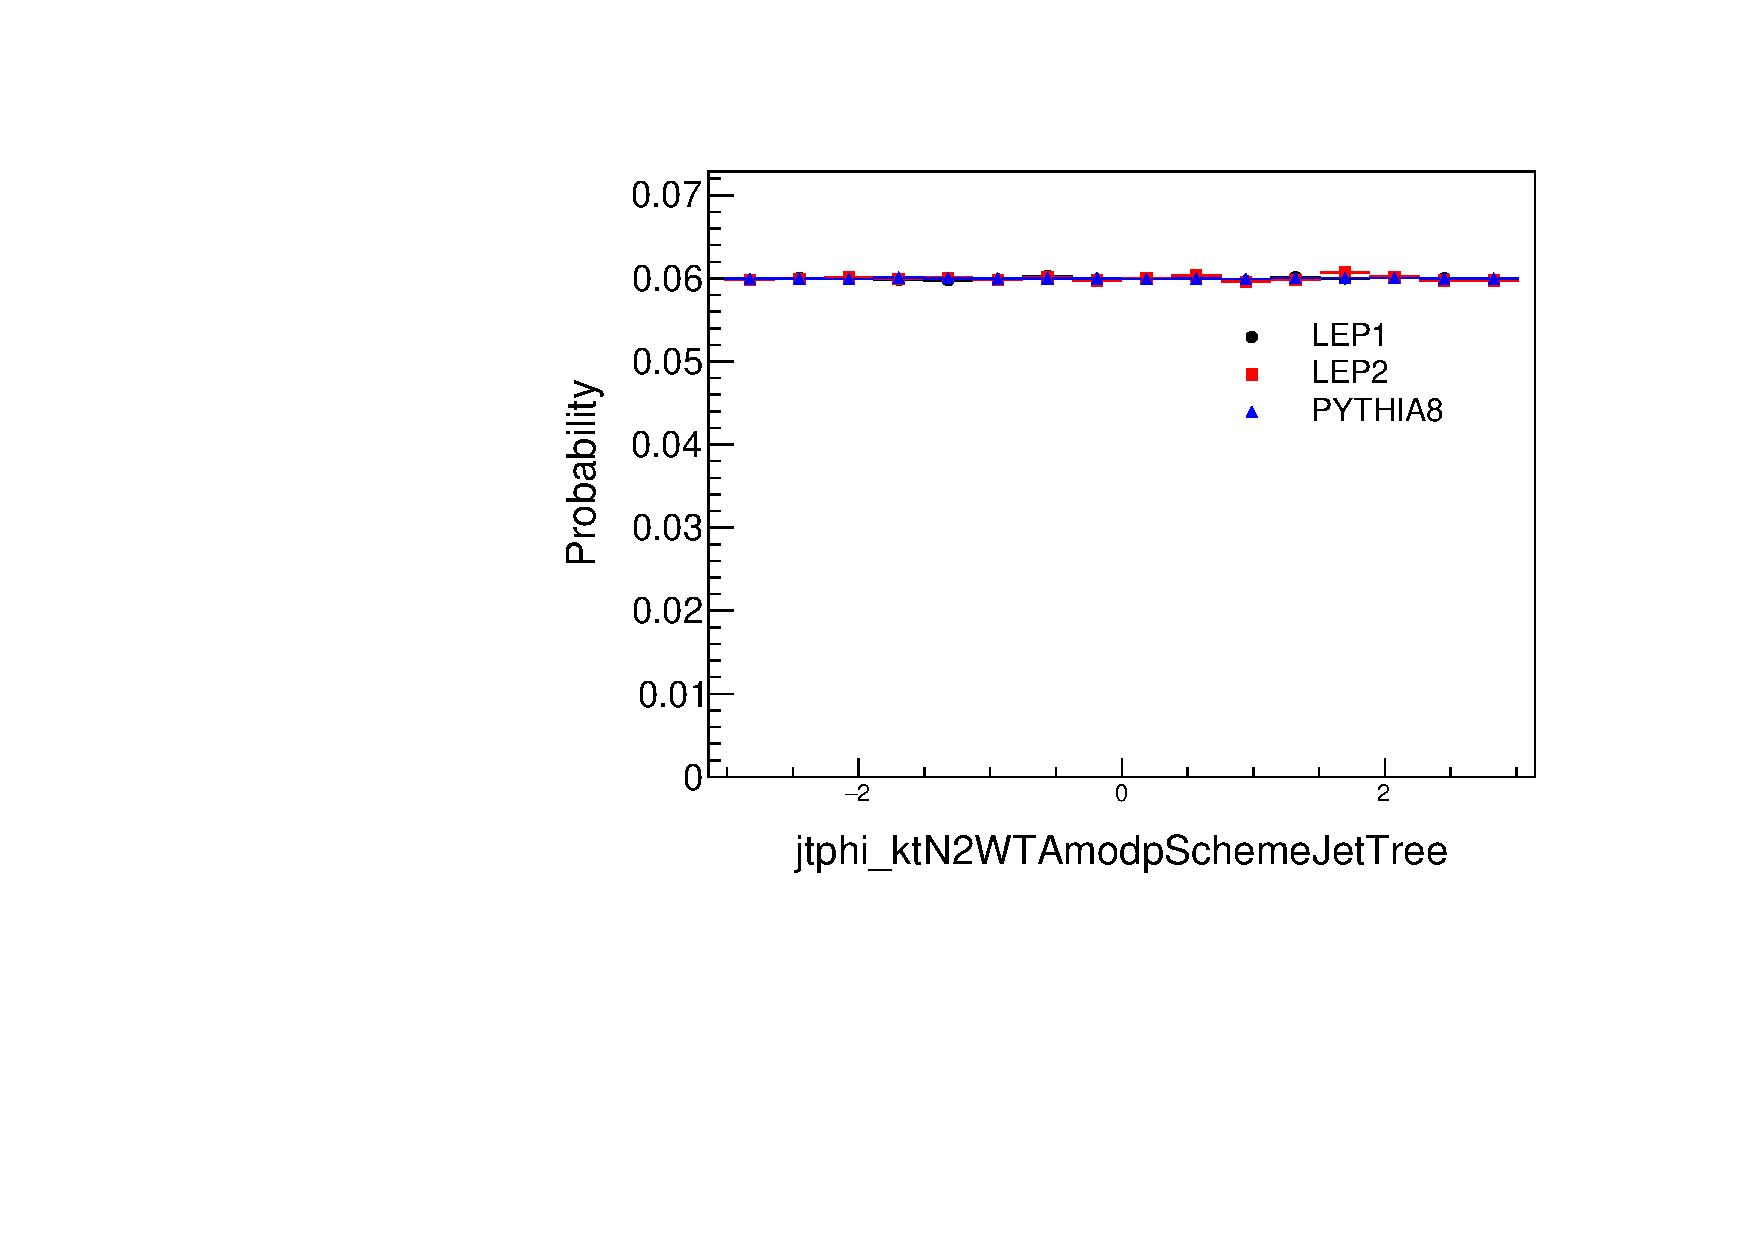
\includegraphics[width=.25\textwidth]{images/DQC/NoCut/jtphi_ktN2WTAmodpSchemeJetTree.pdf}}\hfill
\subfloat{\label{sfig:h}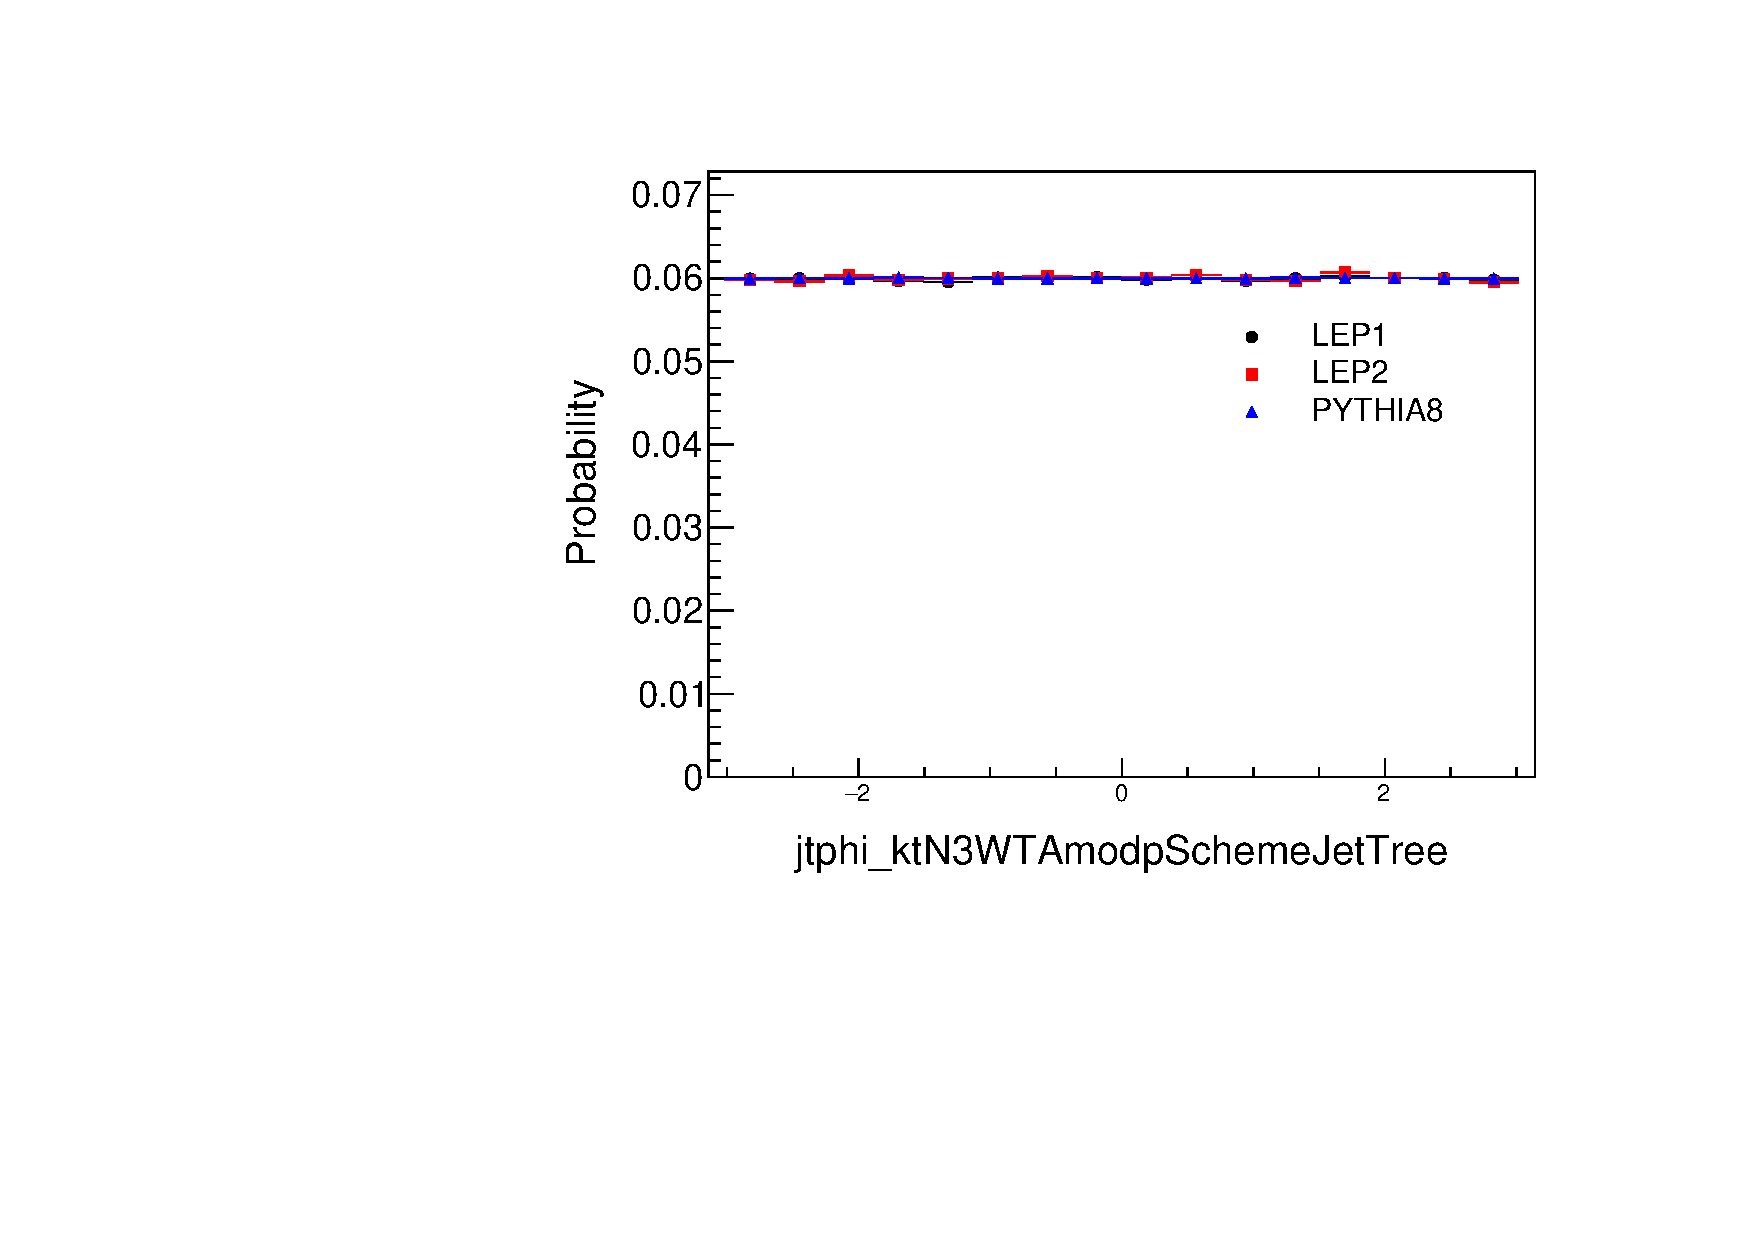
\includegraphics[width=.25\textwidth]{images/DQC/NoCut/jtphi_ktN3WTAmodpSchemeJetTree.pdf}}\hfill
\caption{Raw Data: LEP1, LEP2, Pythia8 no cuts. Jet $\phi$ distributions. Top row: anti-$k_t$, left to right: $R=0.4$, $E$ scheme; $R=0.8$, $E$ scheme; $R=0.4$, WTA mod p scheme; $R=0.8$, WTA mod p scheme. Bottom row: $k_t$, left to right: $N=2$, $E$ scheme; $N=3$, $E$ scheme; $N=2$, WTA mod p scheme; $N=3$; WTA mod p scheme.}  
\end{figure}

\begin{figure}[H]
\centering
\subfloat{\label{sfig:a}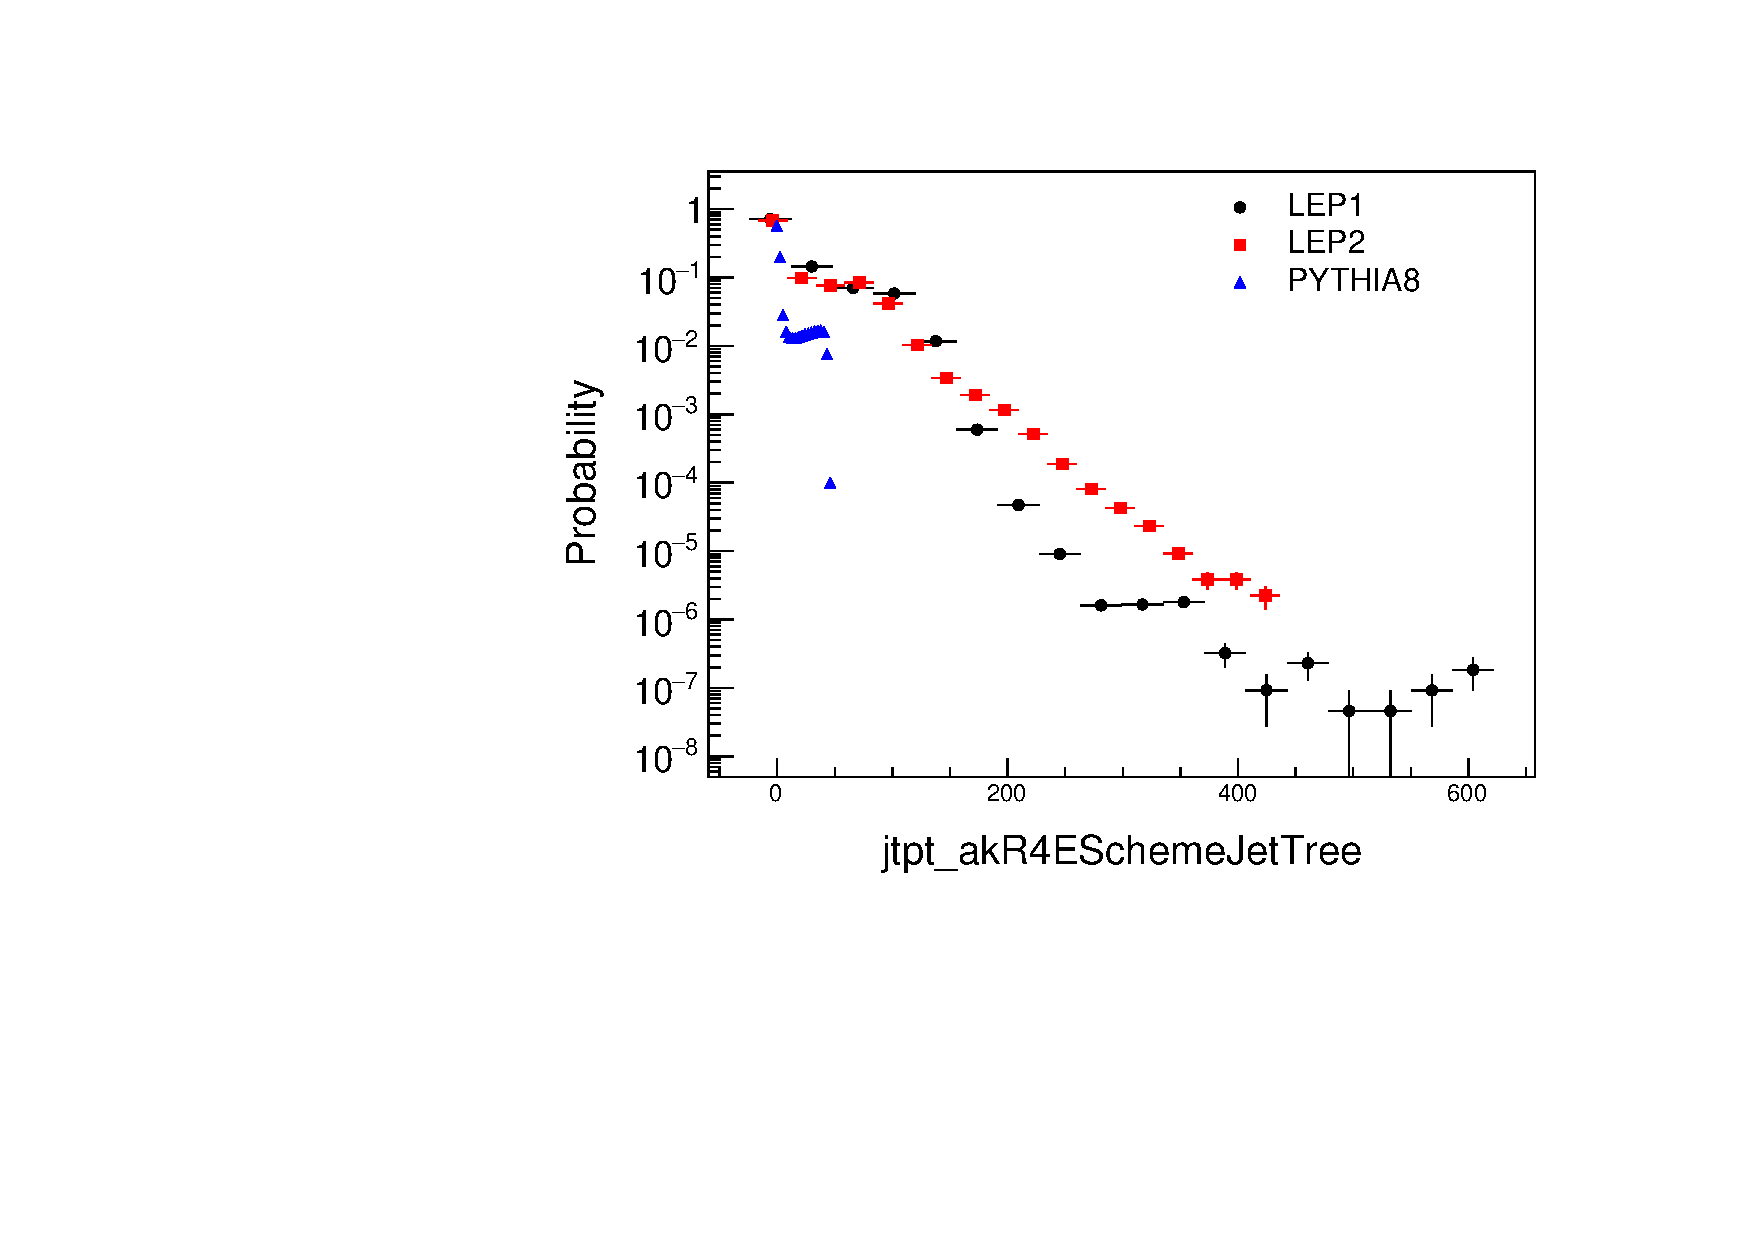
\includegraphics[width=.25\textwidth]{images/DQC/NoCut/jtpt_akR4ESchemeJetTree.pdf}}\hfill
\subfloat{\label{sfig:b}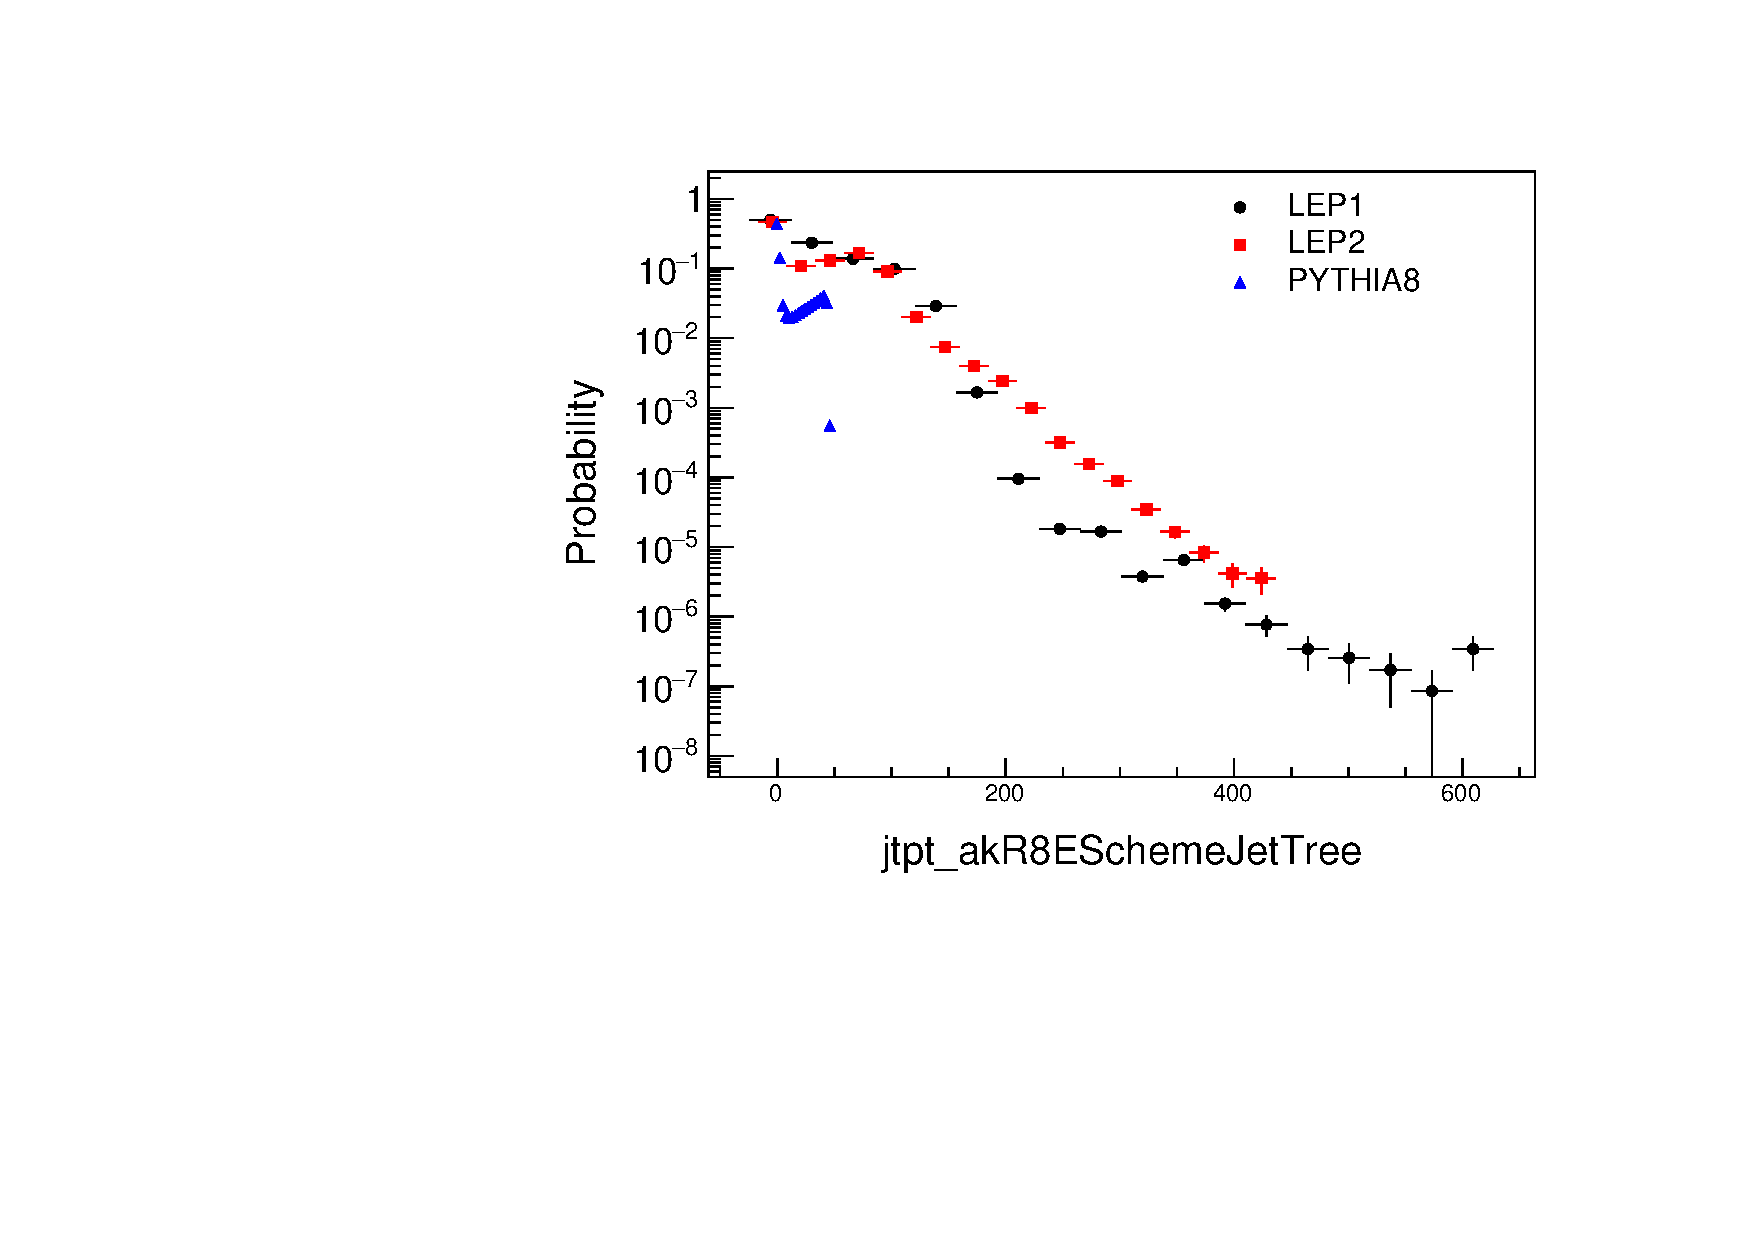
\includegraphics[width=.25\textwidth]{images/DQC/NoCut/jtpt_akR8ESchemeJetTree.pdf}}\hfill
\subfloat{\label{sfig:c}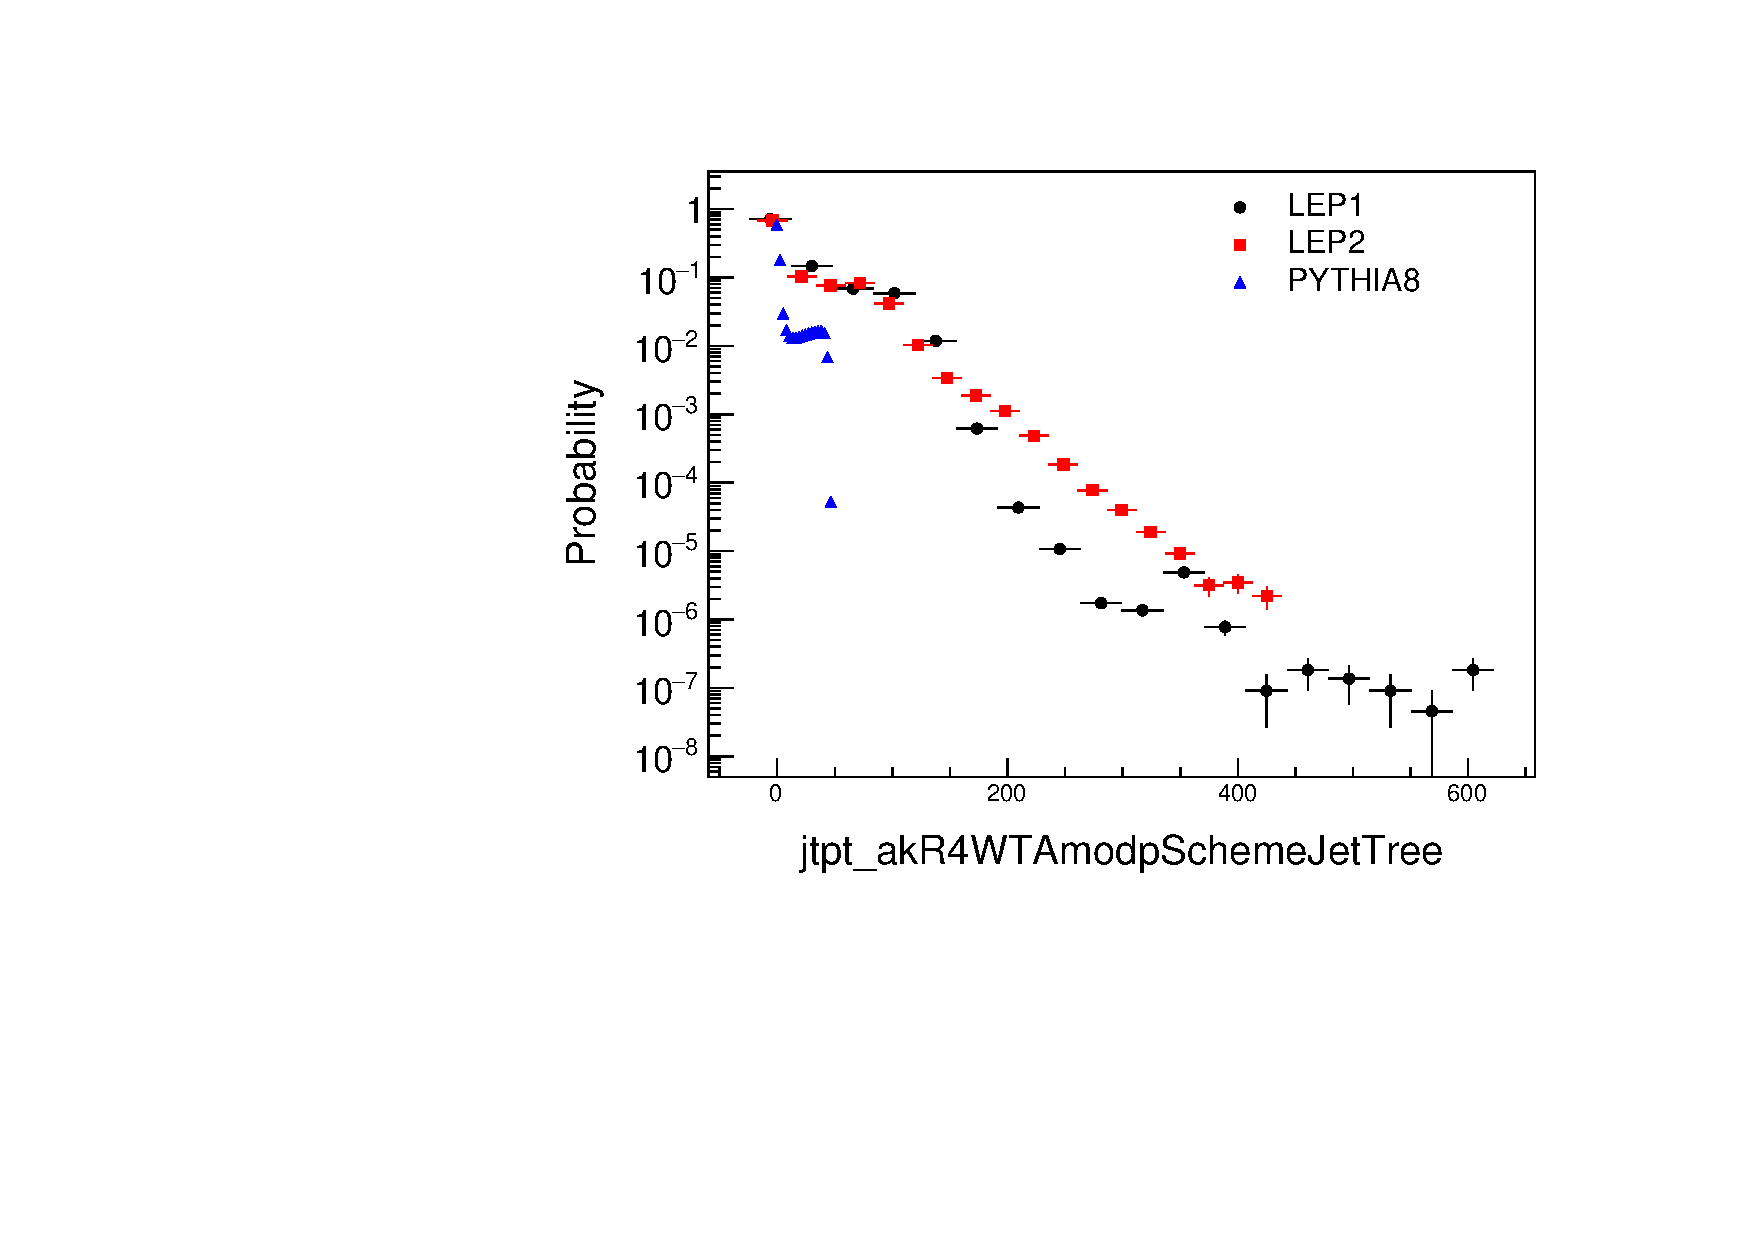
\includegraphics[width=.25\textwidth]{images/DQC/NoCut/jtpt_akR4WTAmodpSchemeJetTree.pdf}}\hfill
\subfloat{\label{sfig:d}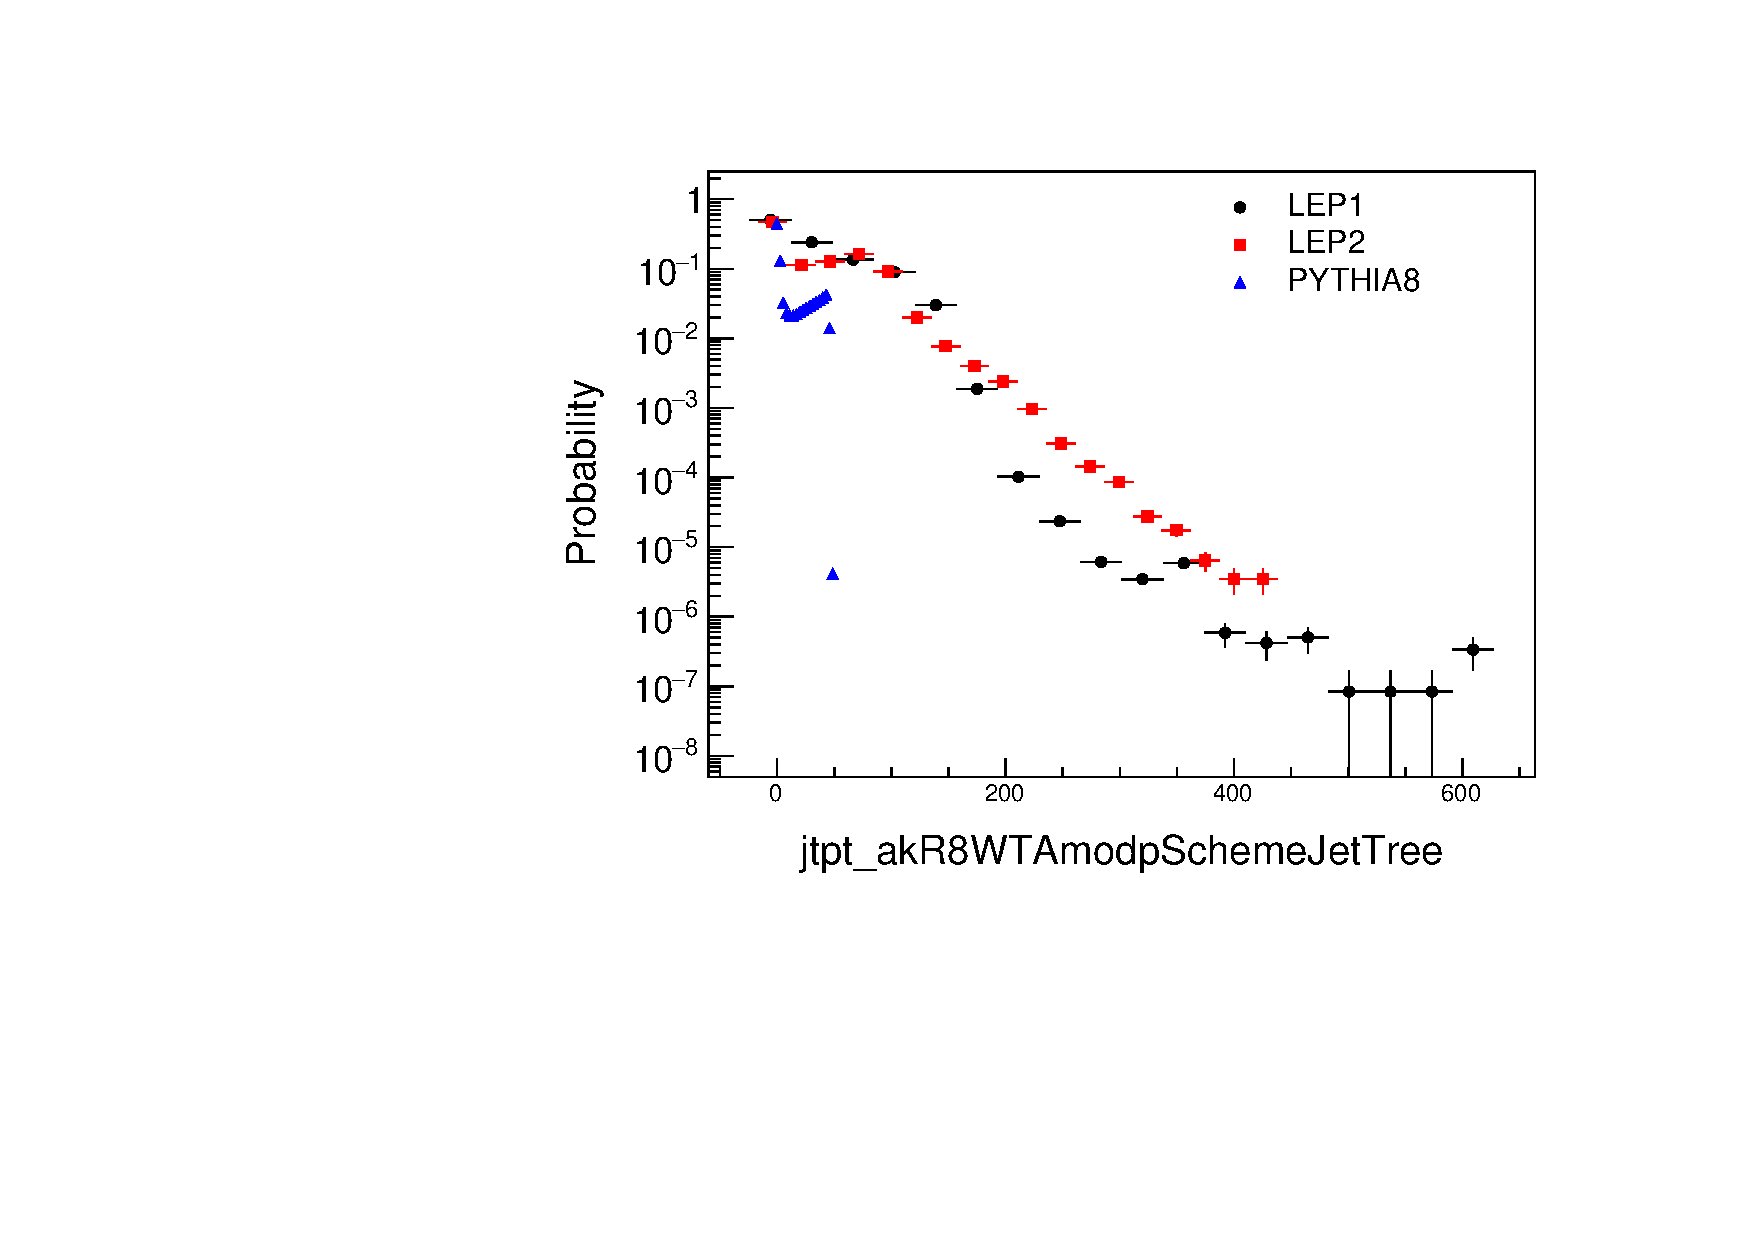
\includegraphics[width=.25\textwidth]{images/DQC/NoCut/jtpt_akR8WTAmodpSchemeJetTree.pdf}}\hfill %row end
\subfloat{\label{sfig:e}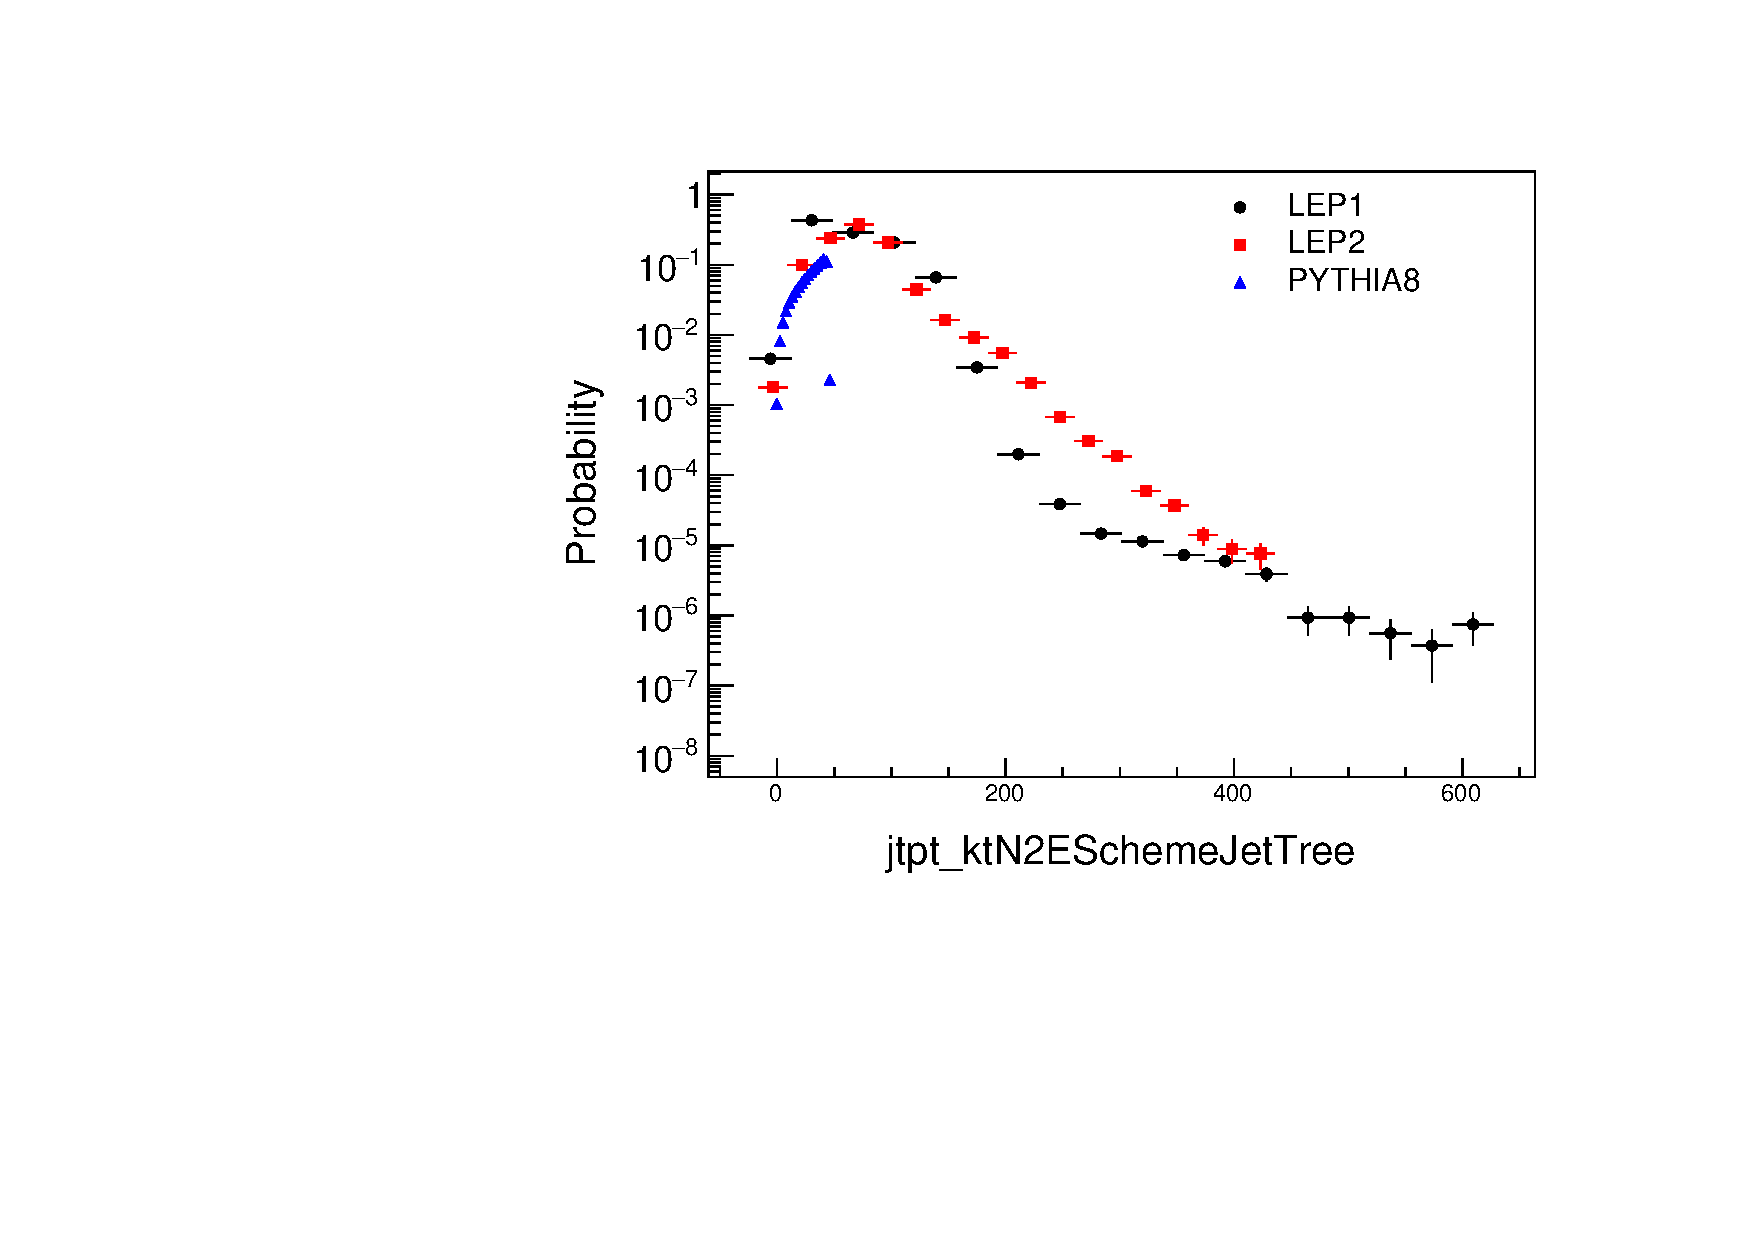
\includegraphics[width=.25\textwidth]{images/DQC/NoCut/jtpt_ktN2ESchemeJetTree.pdf}}\hfill
\subfloat{\label{sfig:f}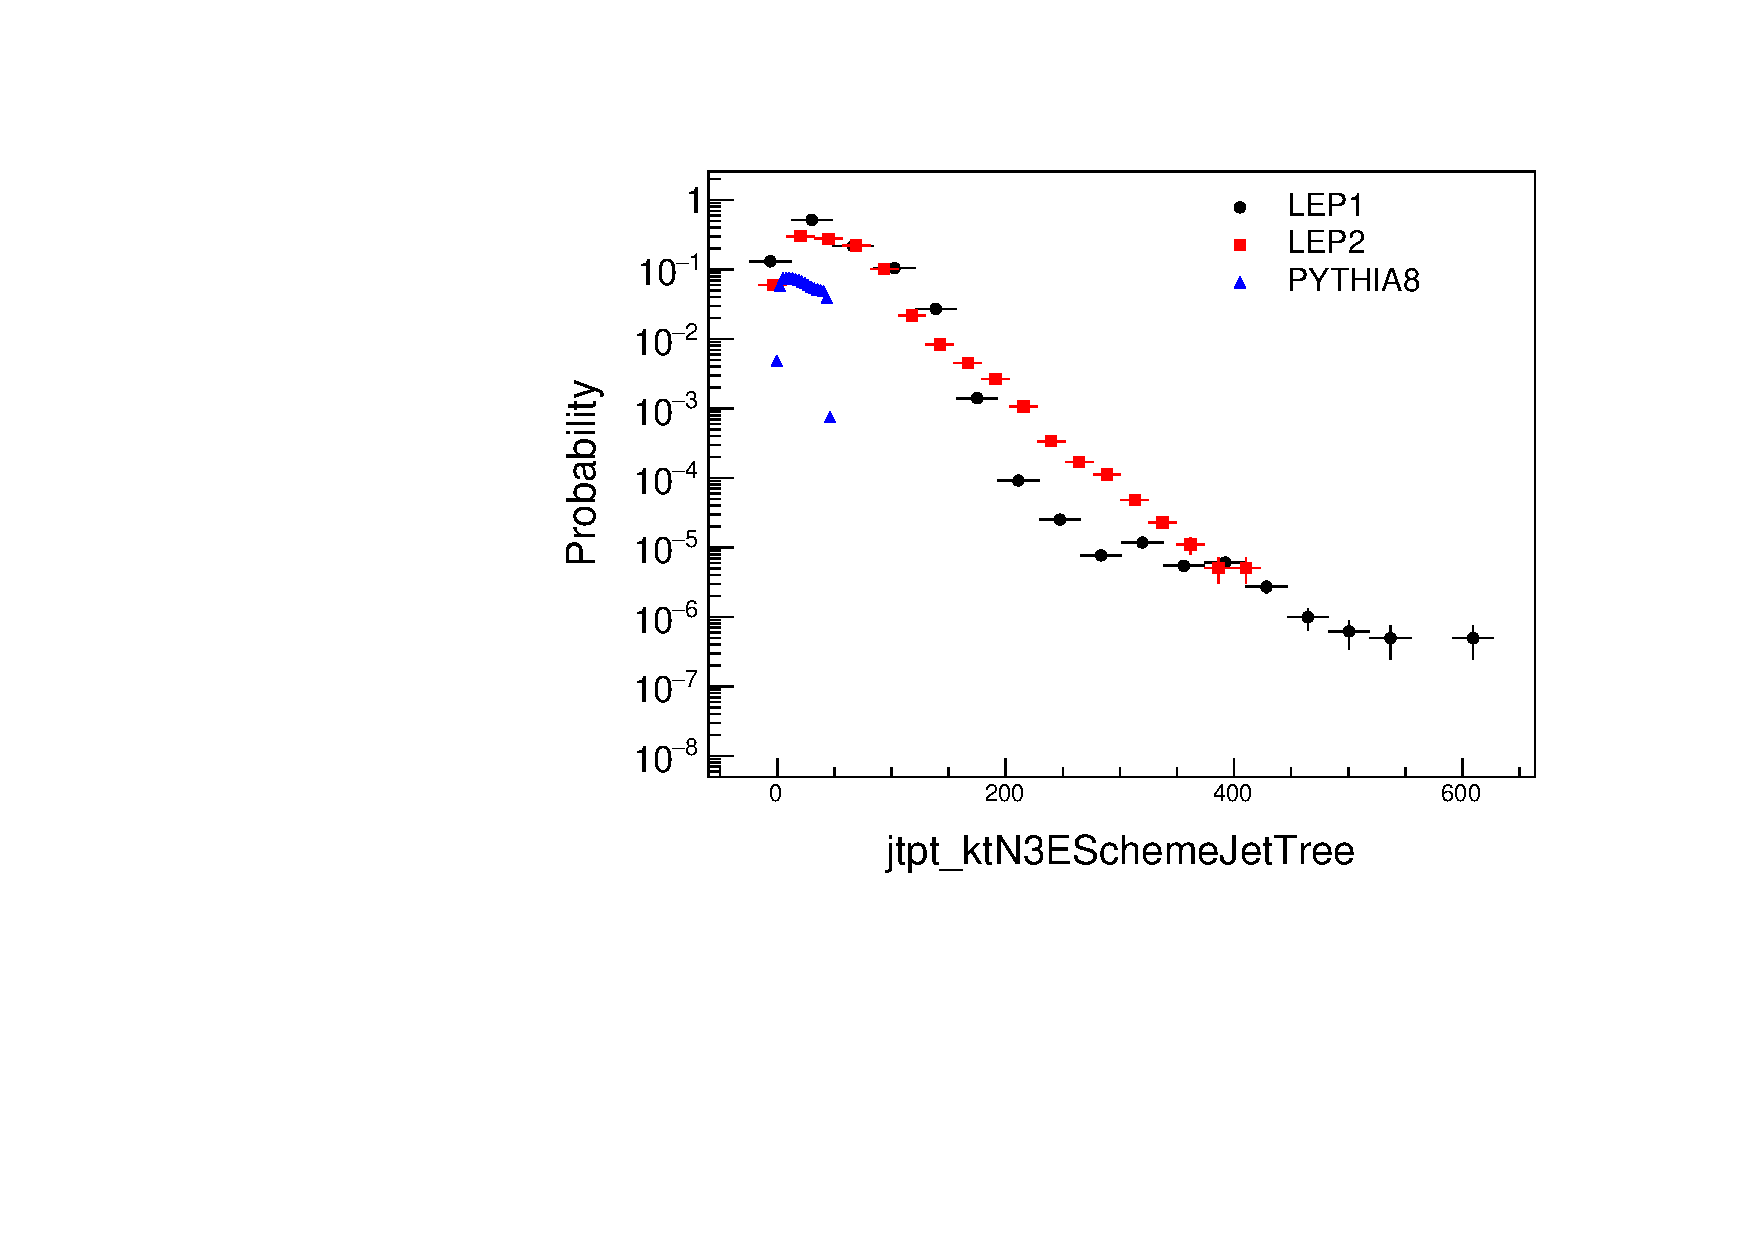
\includegraphics[width=.25\textwidth]{images/DQC/NoCut/jtpt_ktN3ESchemeJetTree.pdf}}\hfill
\subfloat{\label{sfig:g}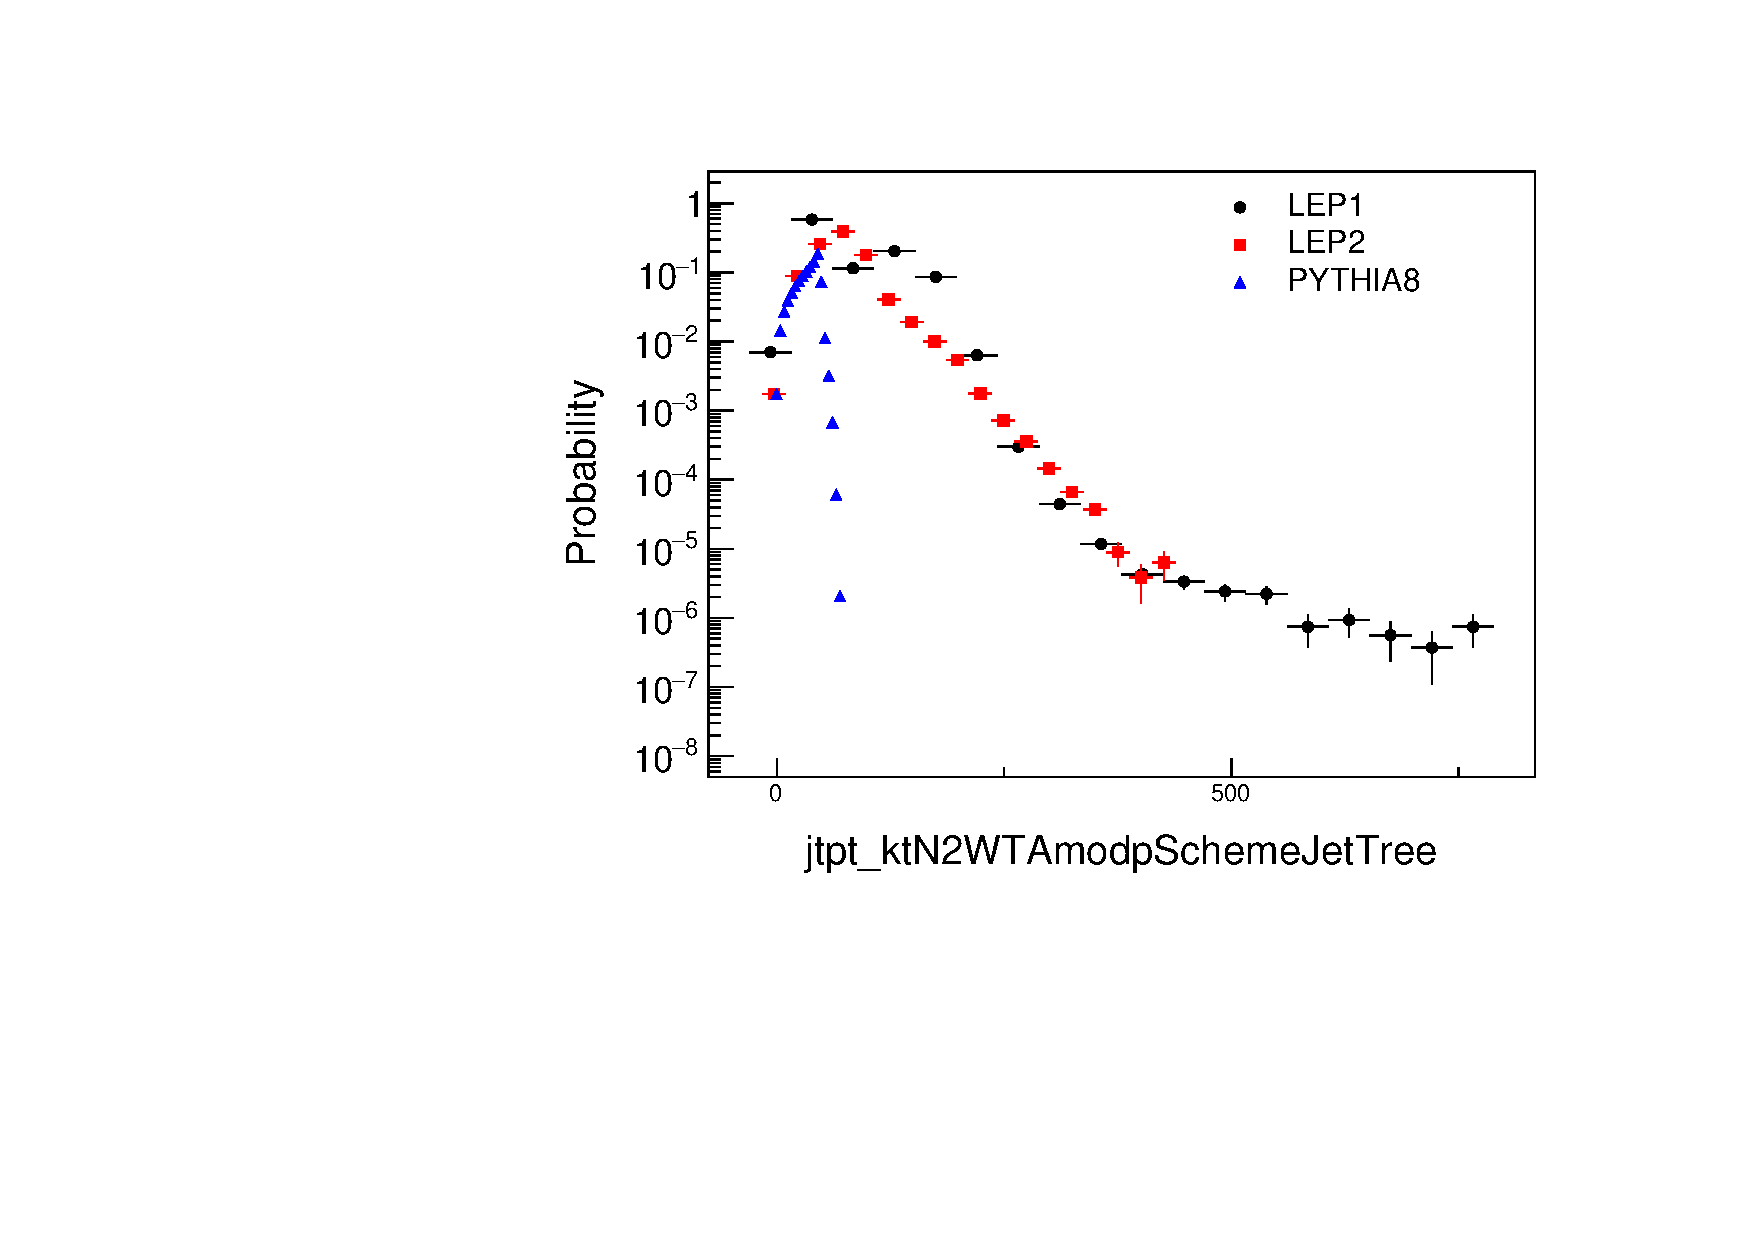
\includegraphics[width=.25\textwidth]{images/DQC/NoCut/jtpt_ktN2WTAmodpSchemeJetTree.pdf}}\hfill
\subfloat{\label{sfig:h}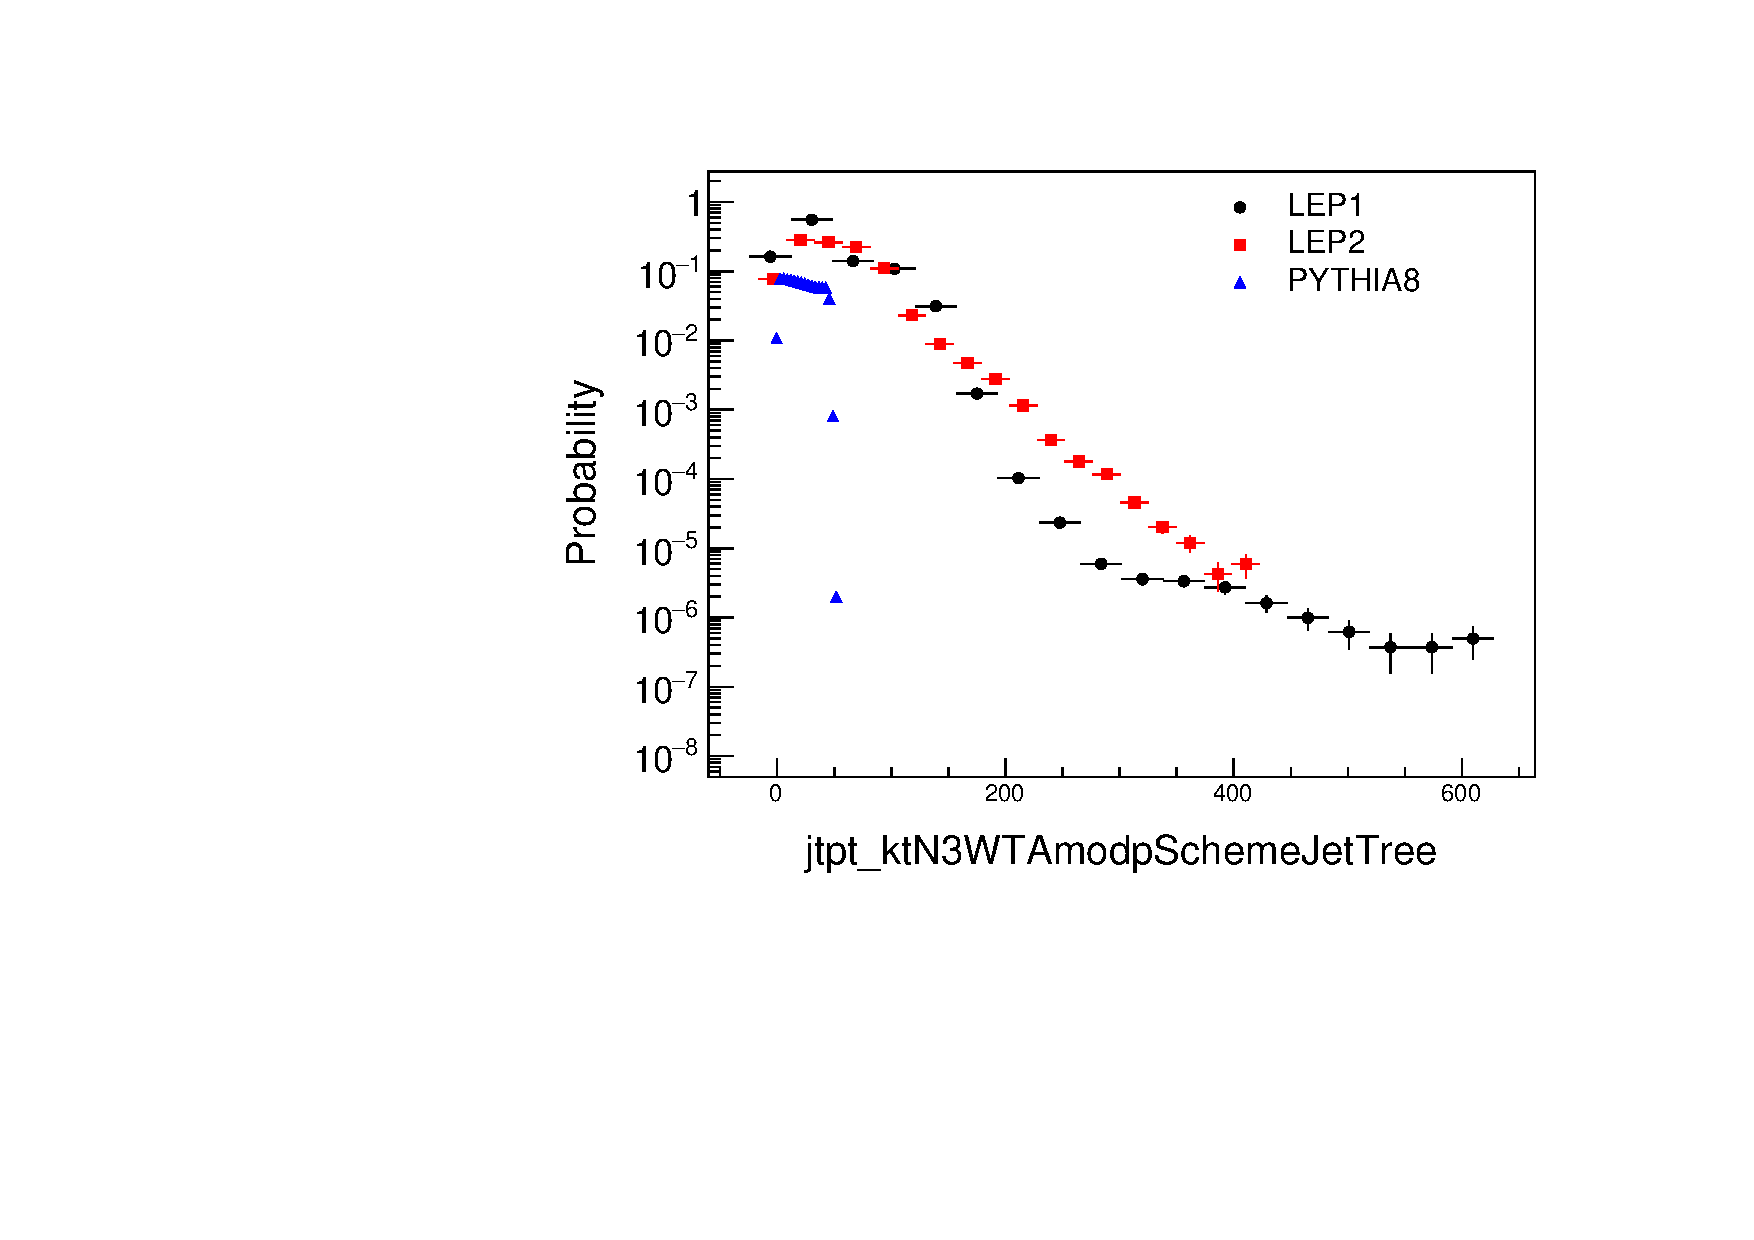
\includegraphics[width=.25\textwidth]{images/DQC/NoCut/jtpt_ktN3WTAmodpSchemeJetTree.pdf}}\hfill
\caption{Raw Data: LEP1, LEP2, Pythia8 no cuts. Jet $p_t$ distributions. Top row: anti-$k_t$, left to right: $R=0.4$, $E$ scheme; $R=0.8$, $E$ scheme; $R=0.4$, WTA mod p scheme; $R=0.8$, WTA mod p scheme. Bottom row: $k_t$, left to right: $N=2$, $E$ scheme; $N=3$, $E$ scheme; $N=2$, WTA mod p scheme; $N=3$; WTA mod p scheme.}  
\end{figure}

\begin{figure}[H]
\centering
\subfloat{\label{sfig:a}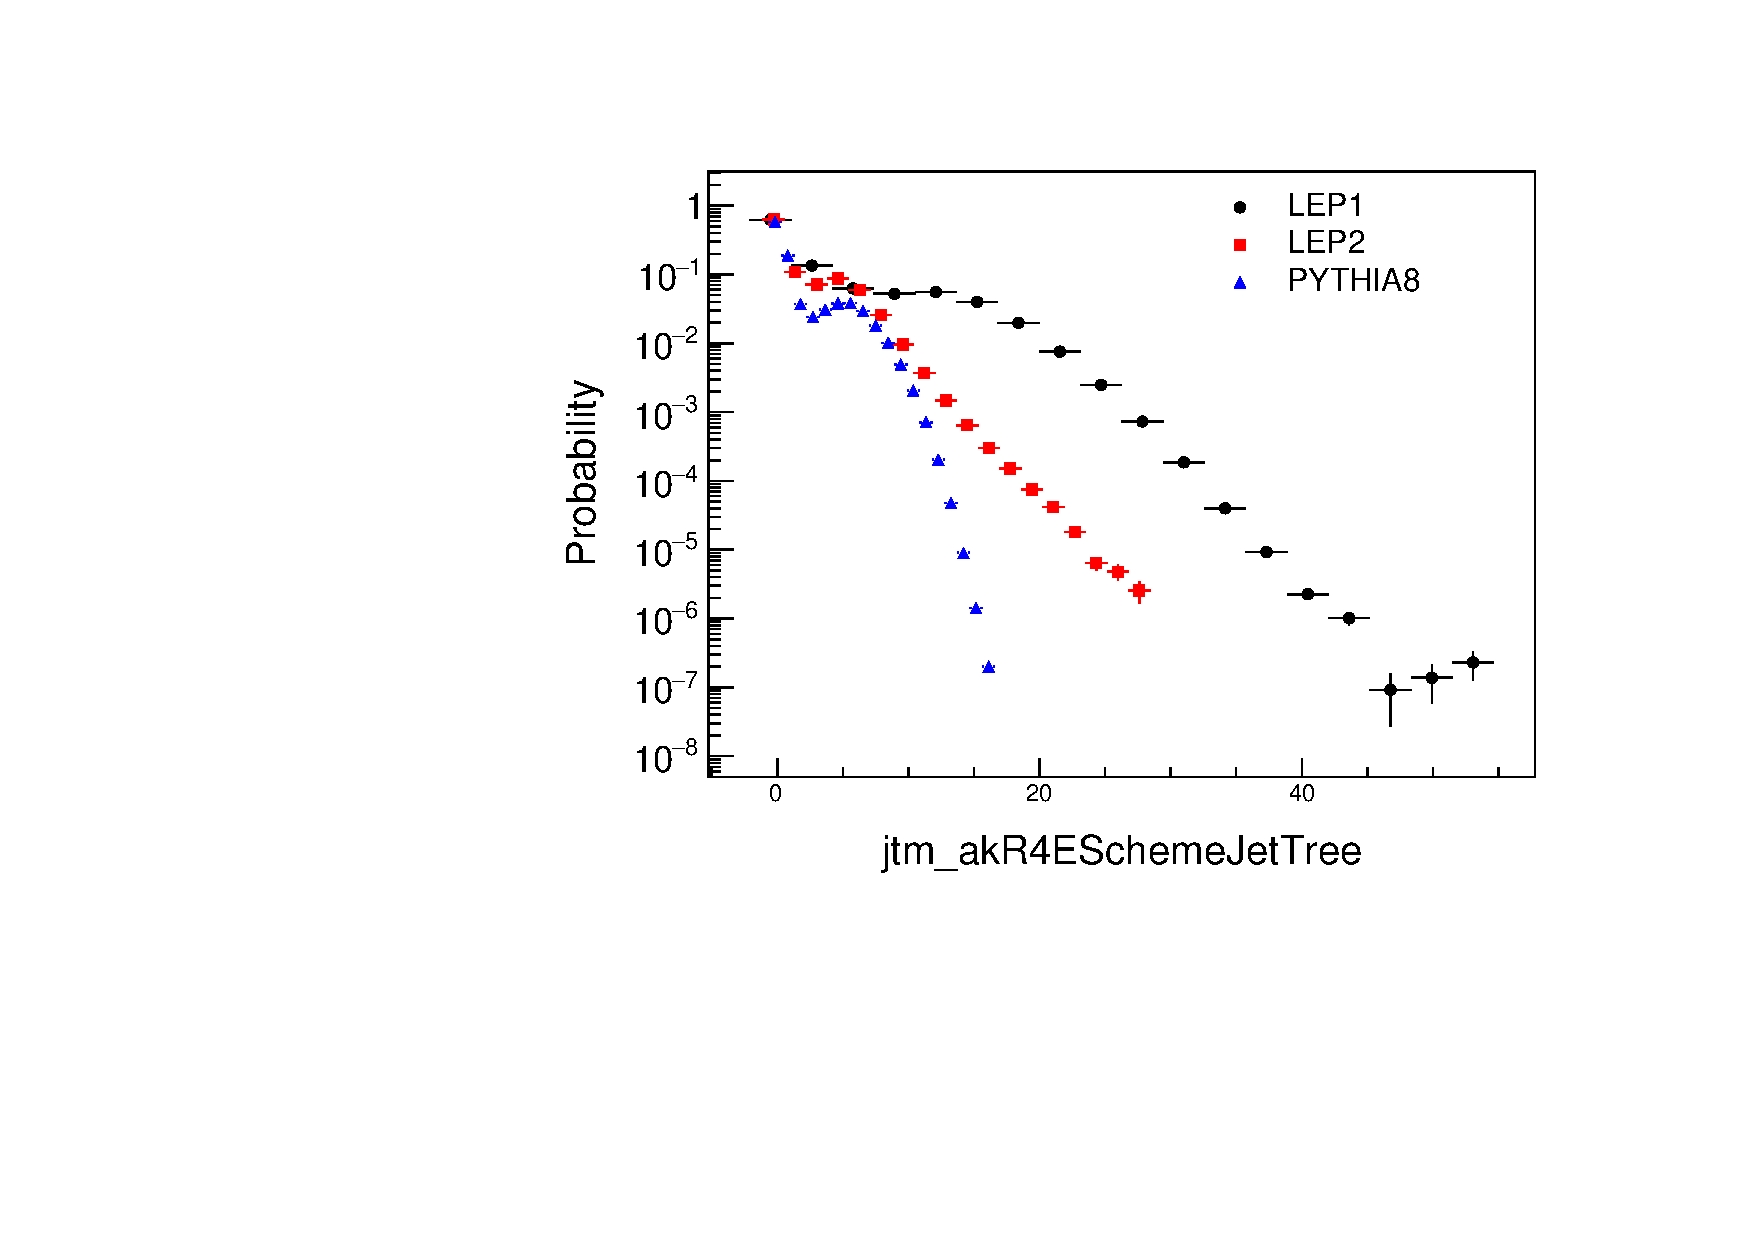
\includegraphics[width=.25\textwidth]{images/DQC/NoCut/jtm_akR4ESchemeJetTree.pdf}}\hfill
\subfloat{\label{sfig:b}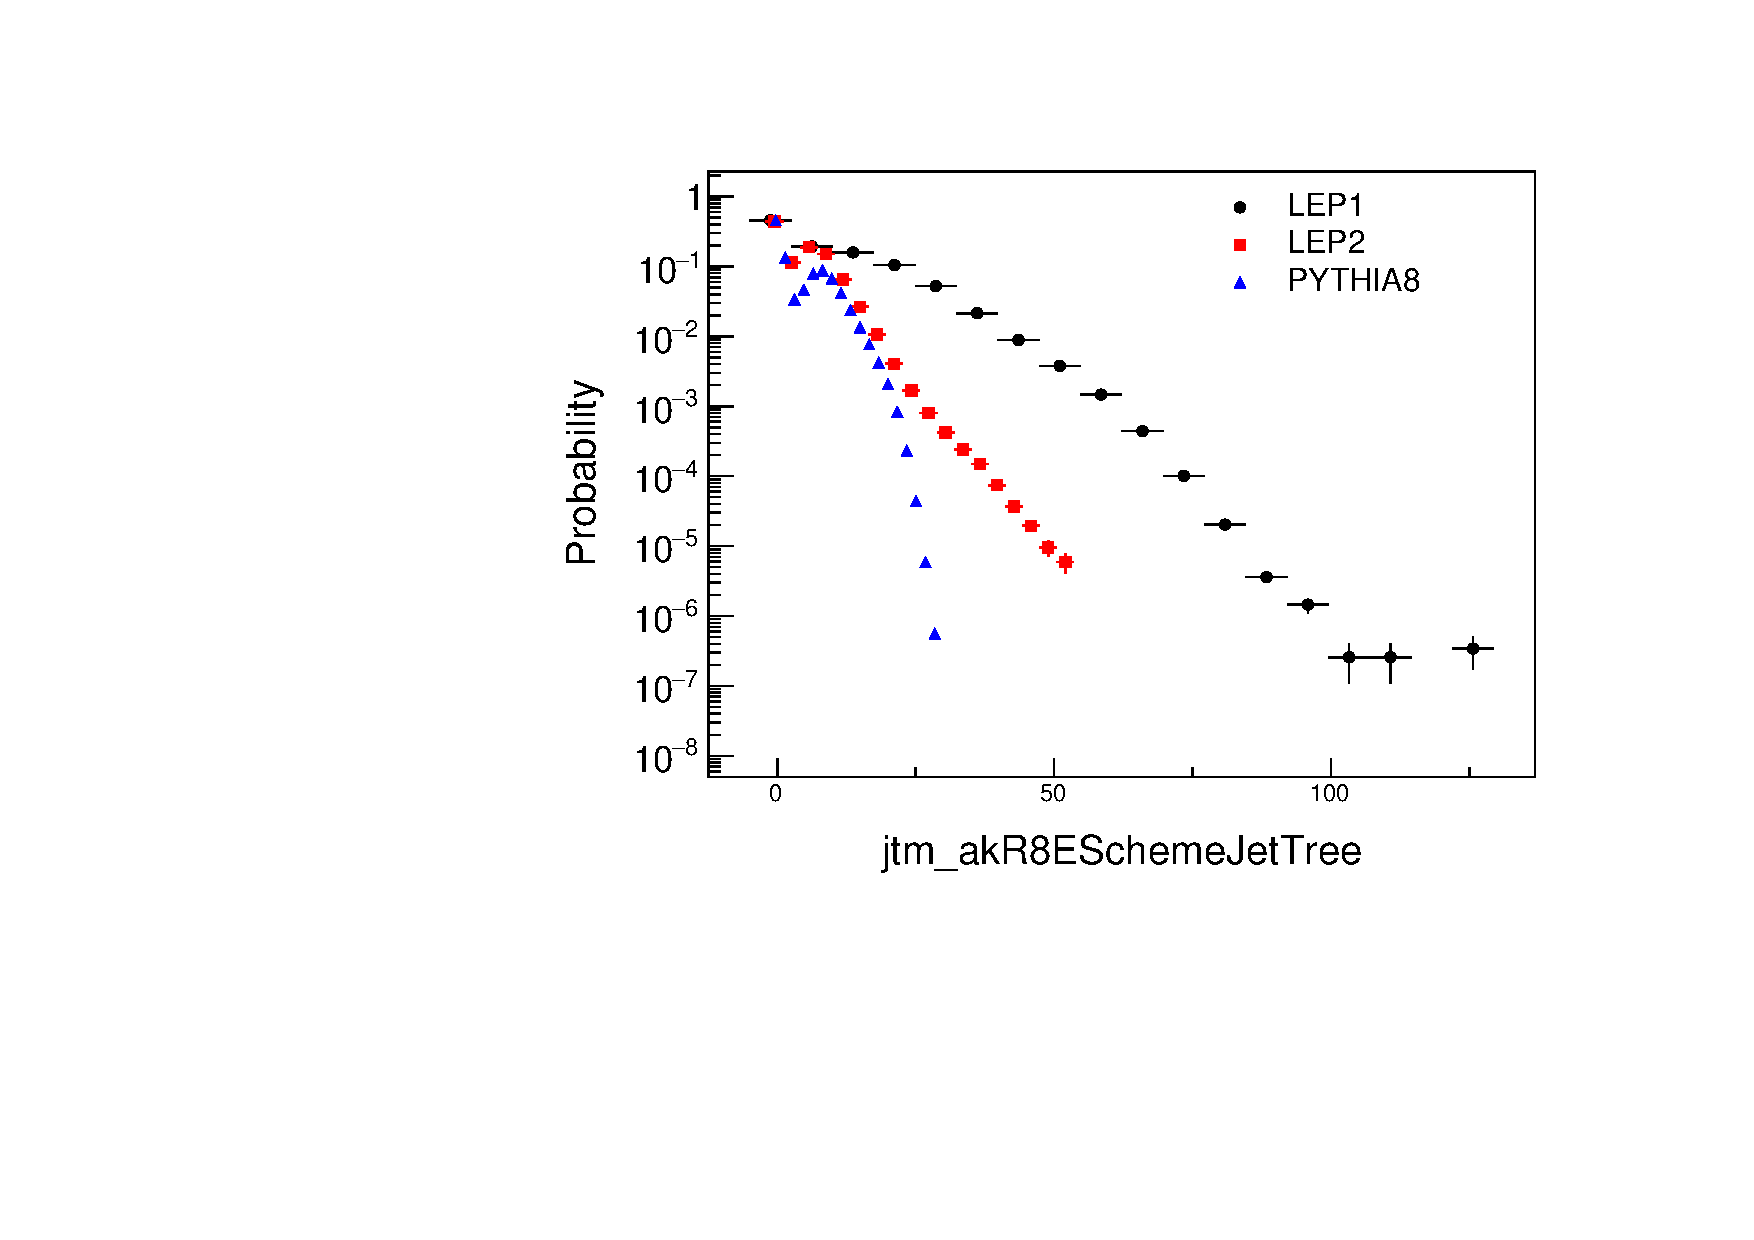
\includegraphics[width=.25\textwidth]{images/DQC/NoCut/jtm_akR8ESchemeJetTree.pdf}}\hfill
\subfloat{\label{sfig:c}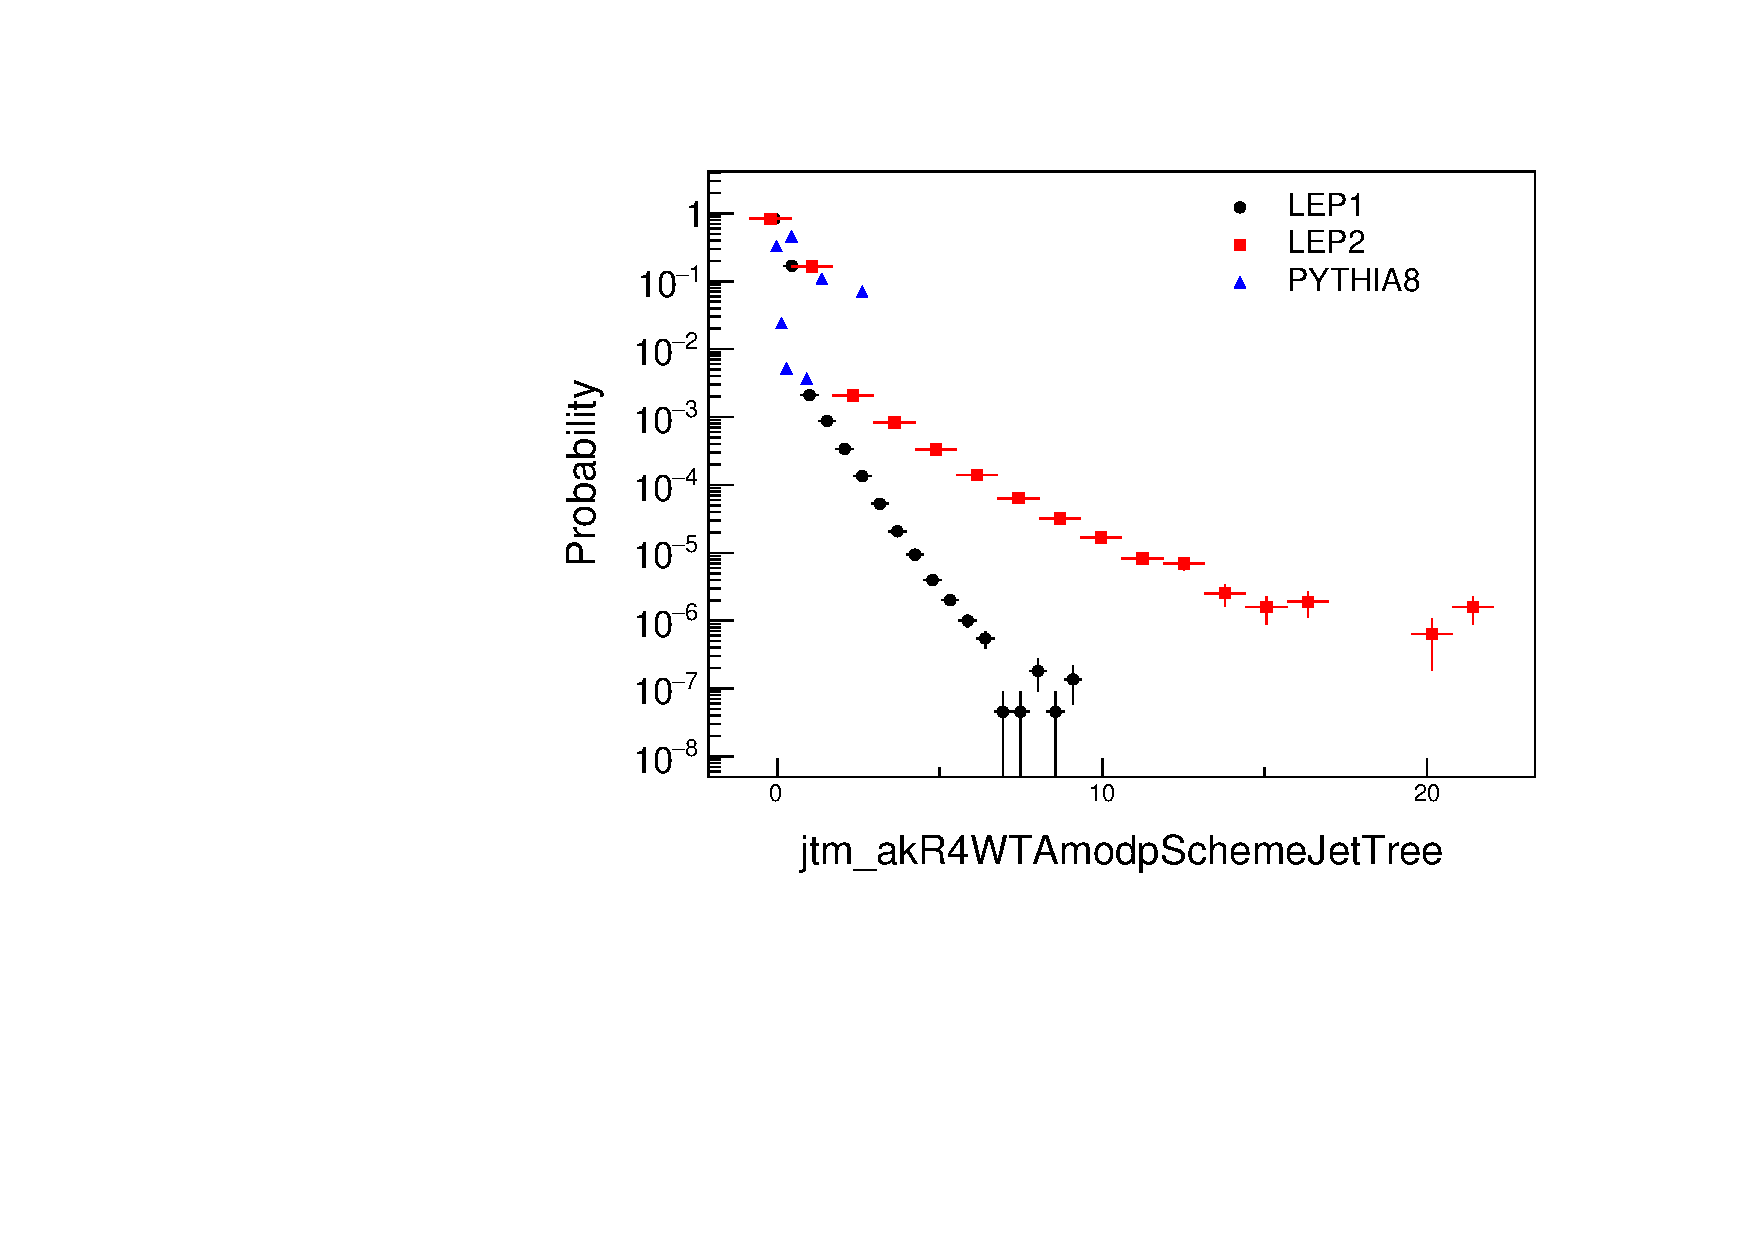
\includegraphics[width=.25\textwidth]{images/DQC/NoCut/jtm_akR4WTAmodpSchemeJetTree.pdf}}\hfill
\subfloat{\label{sfig:d}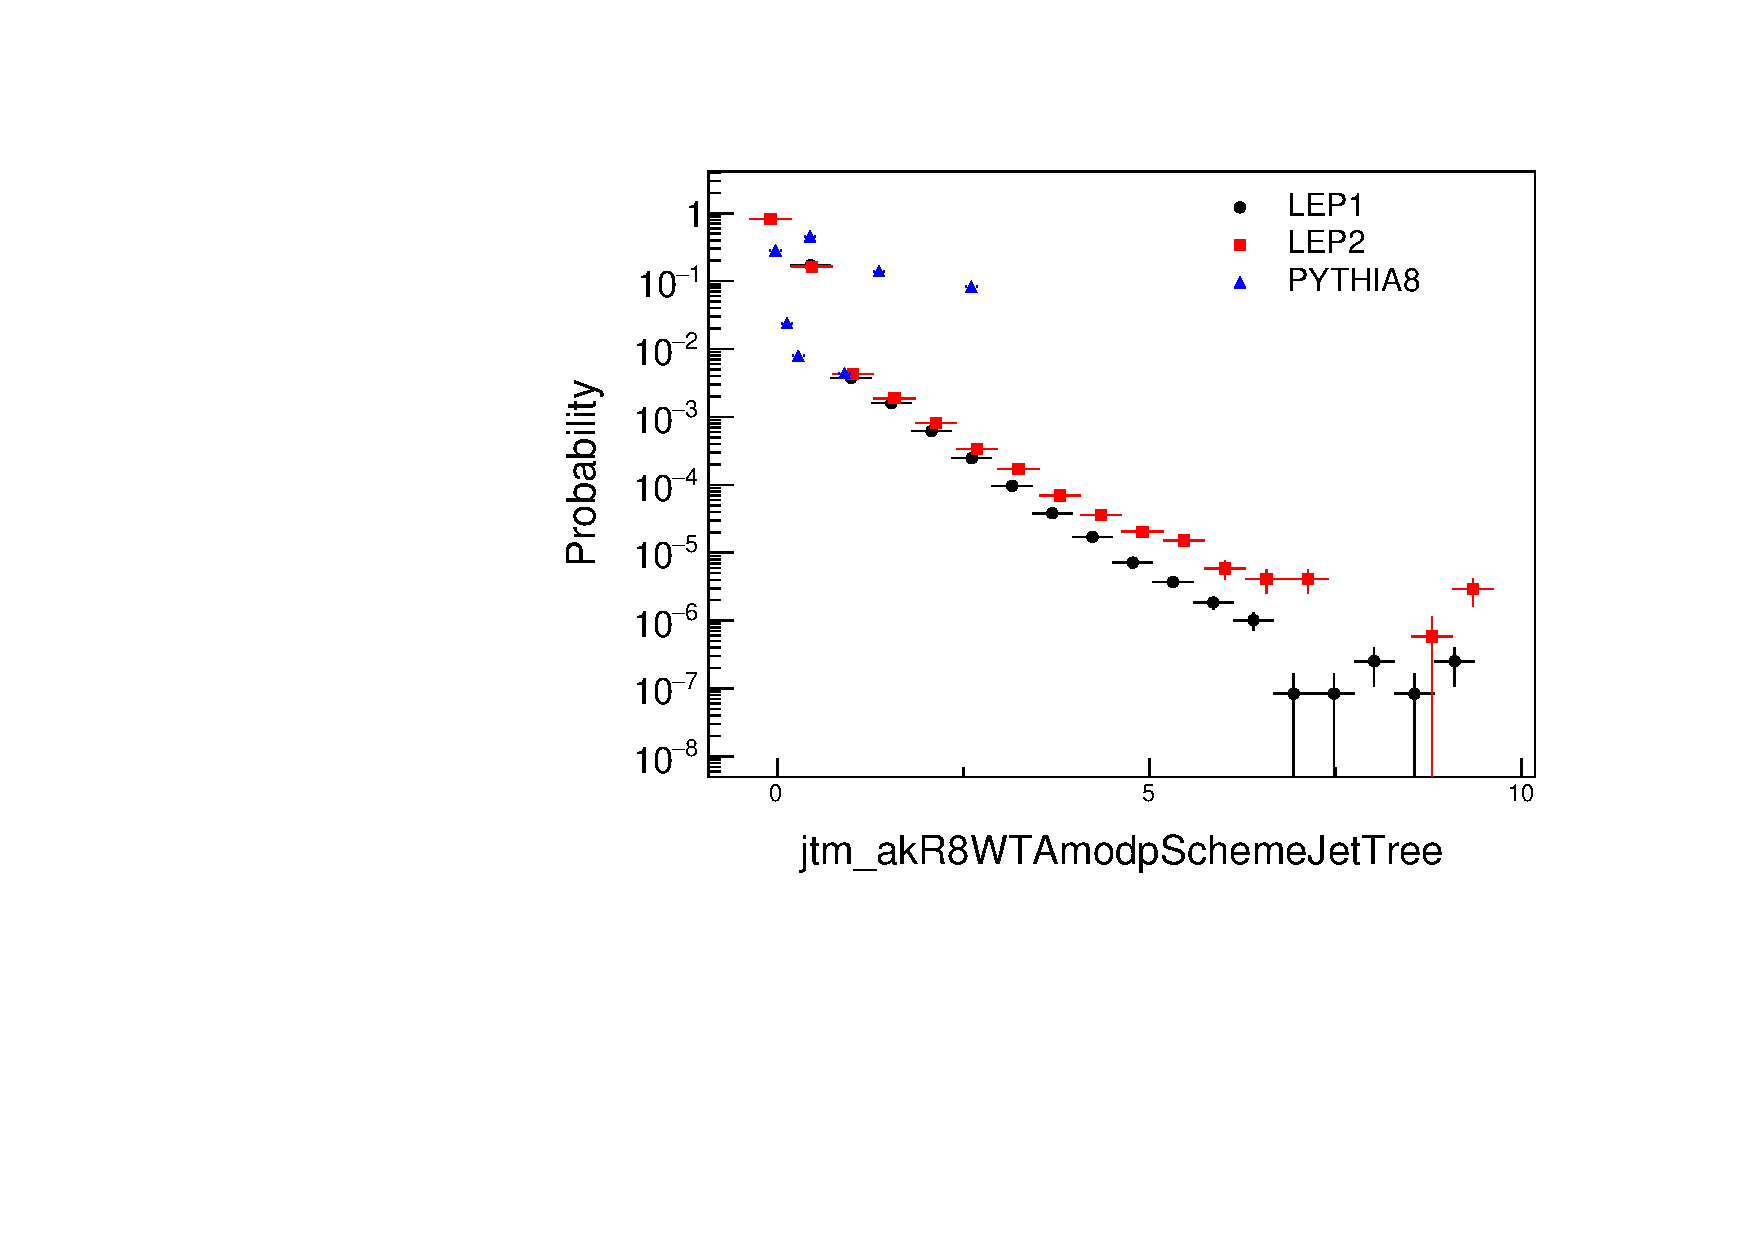
\includegraphics[width=.25\textwidth]{images/DQC/NoCut/jtm_akR8WTAmodpSchemeJetTree.pdf}}\hfill %row end
\subfloat{\label{sfig:e}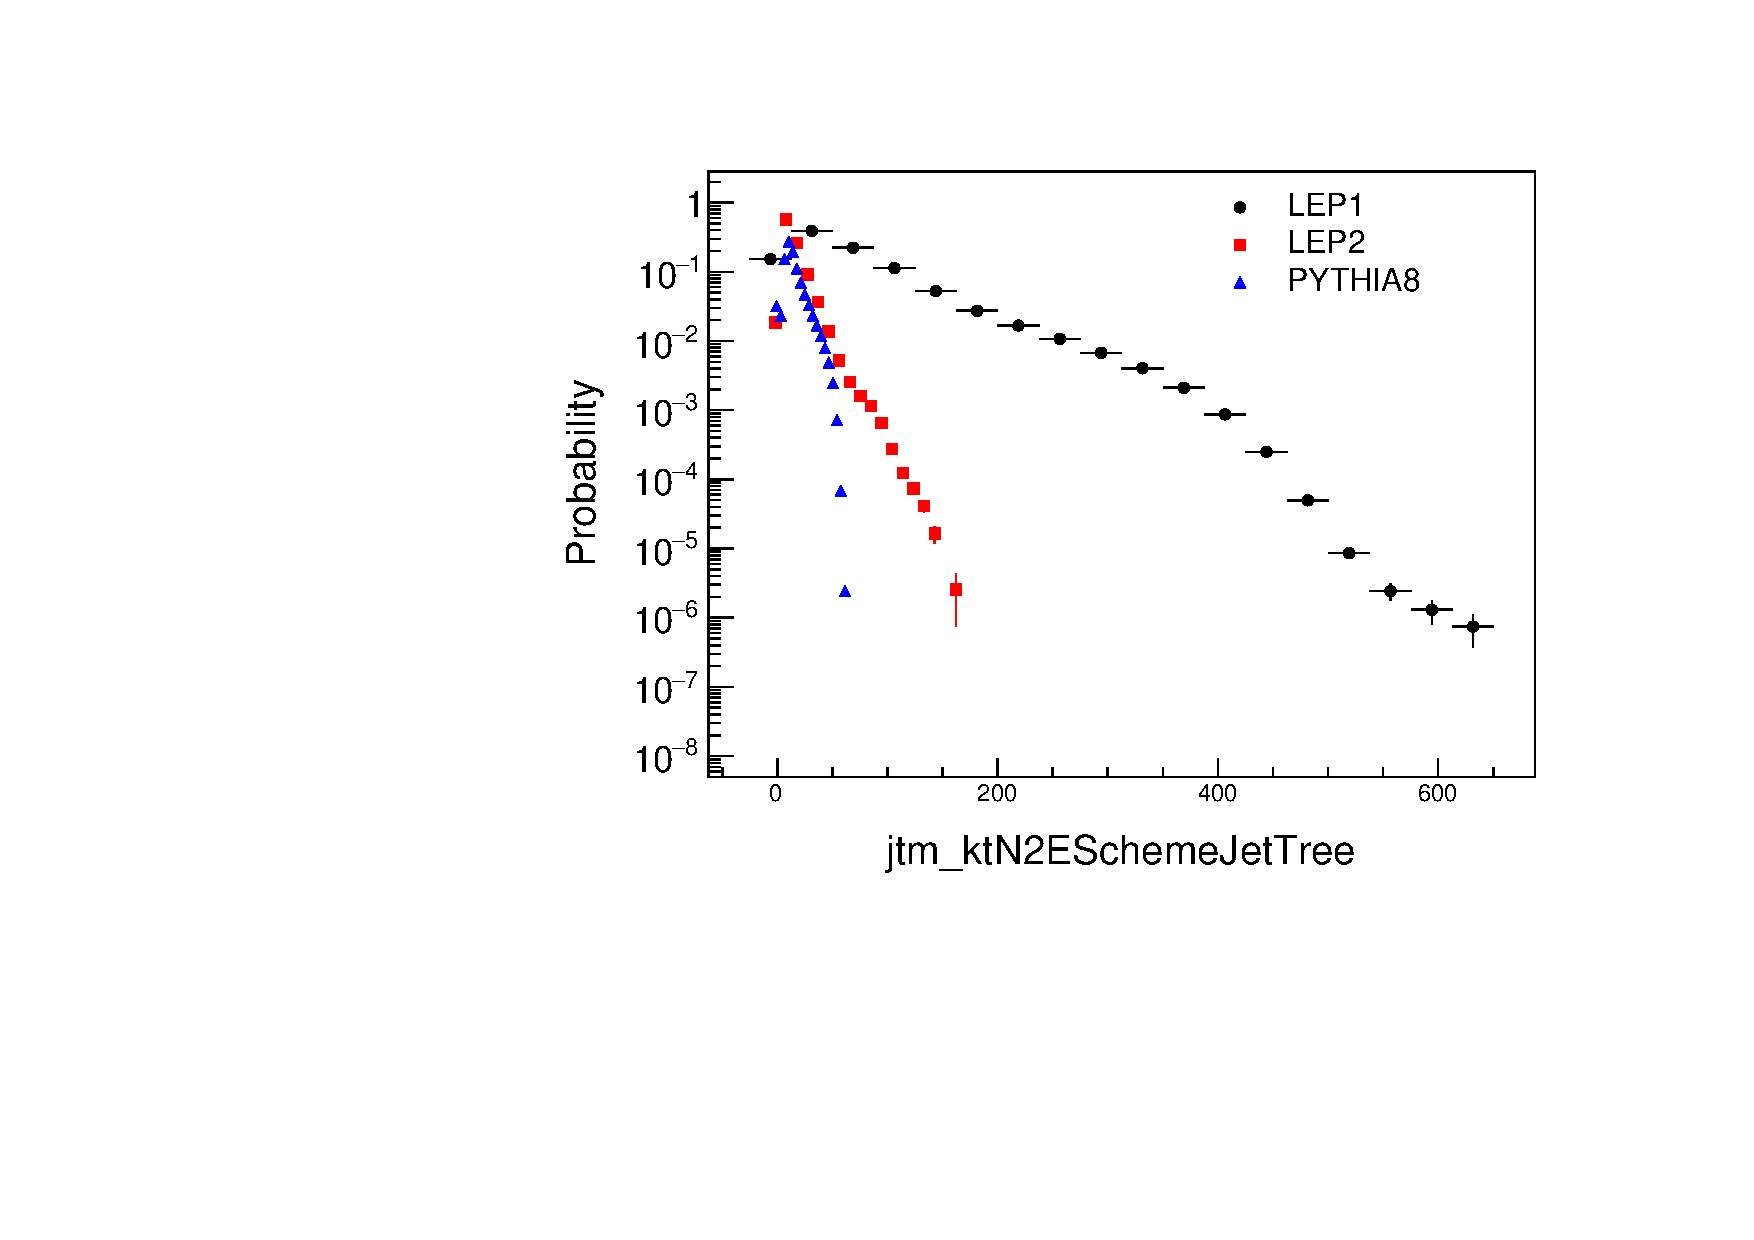
\includegraphics[width=.25\textwidth]{images/DQC/NoCut/jtm_ktN2ESchemeJetTree.pdf}}\hfill
\subfloat{\label{sfig:f}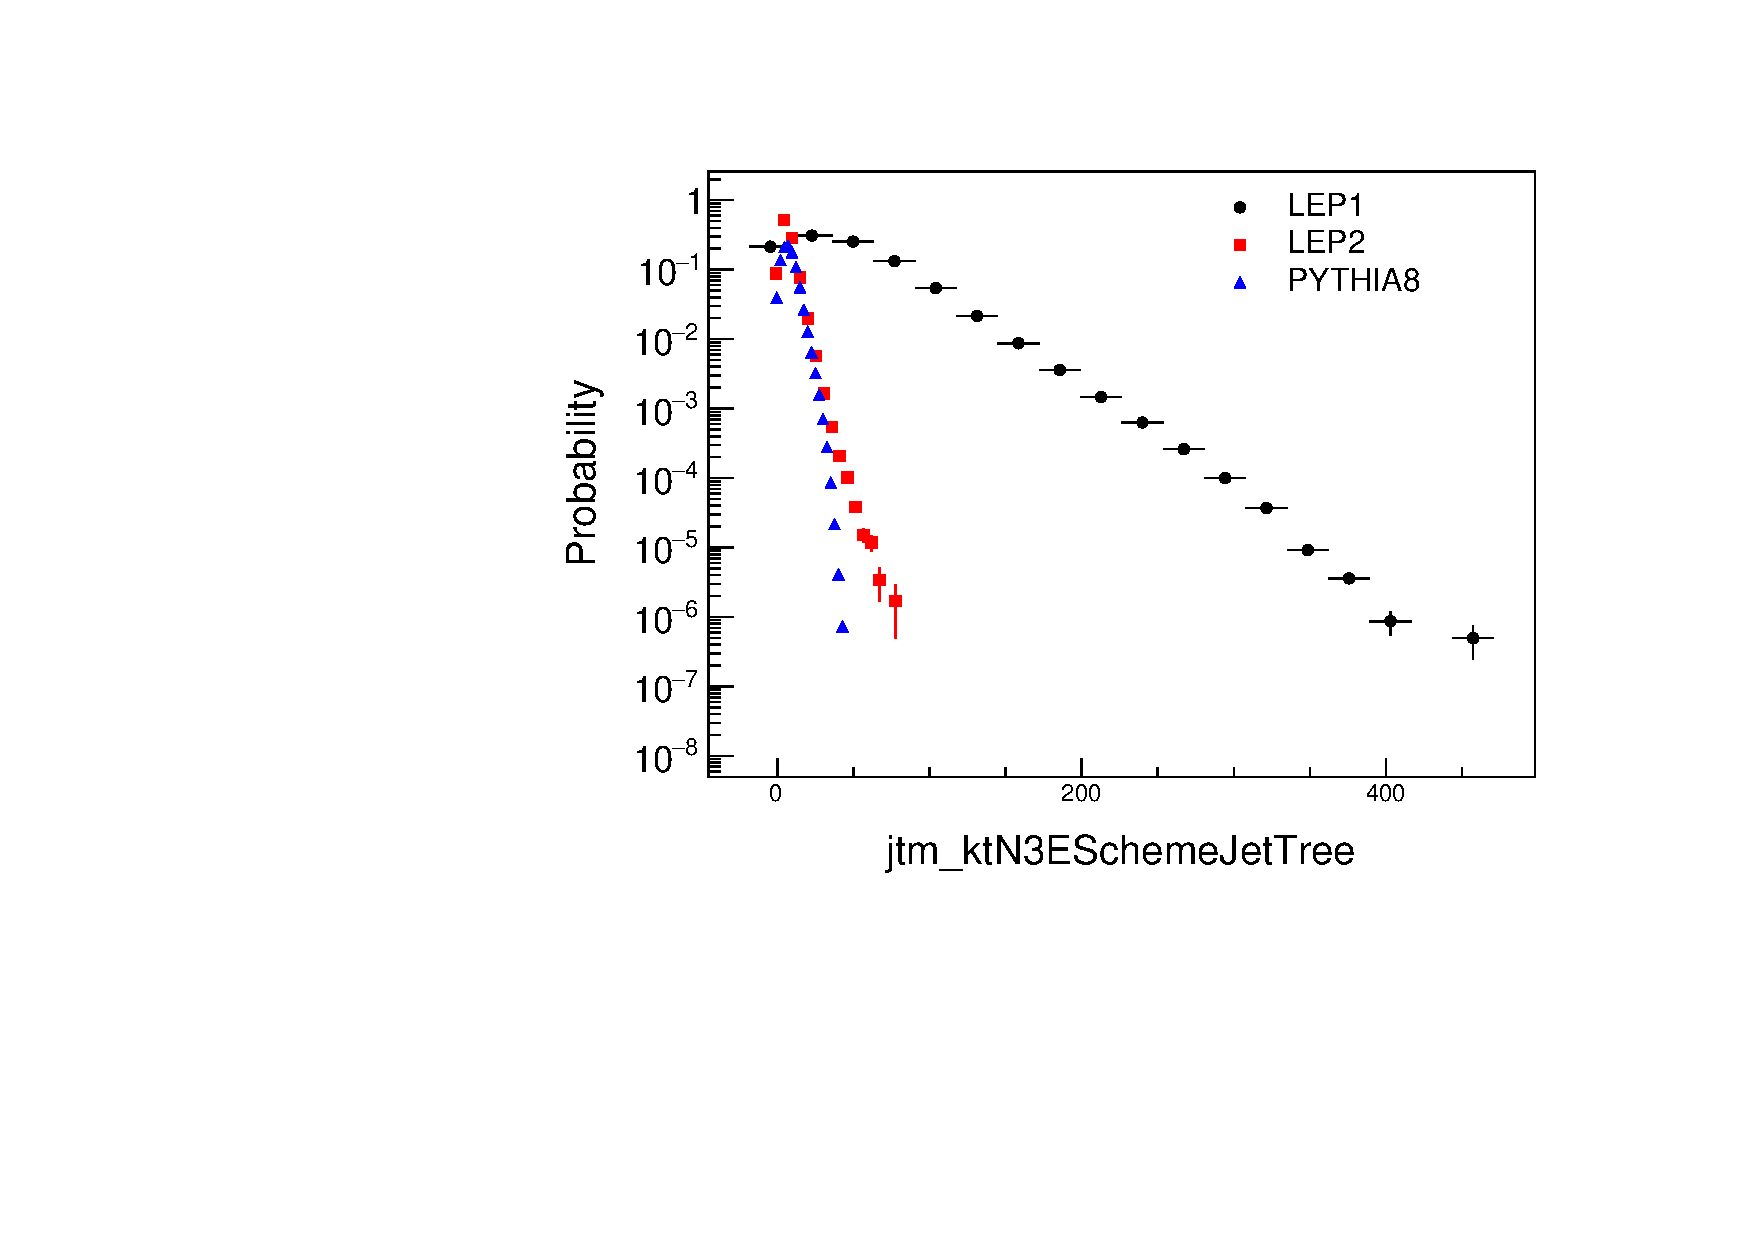
\includegraphics[width=.25\textwidth]{images/DQC/NoCut/jtm_ktN3ESchemeJetTree.pdf}}\hfill
\subfloat{\label{sfig:g}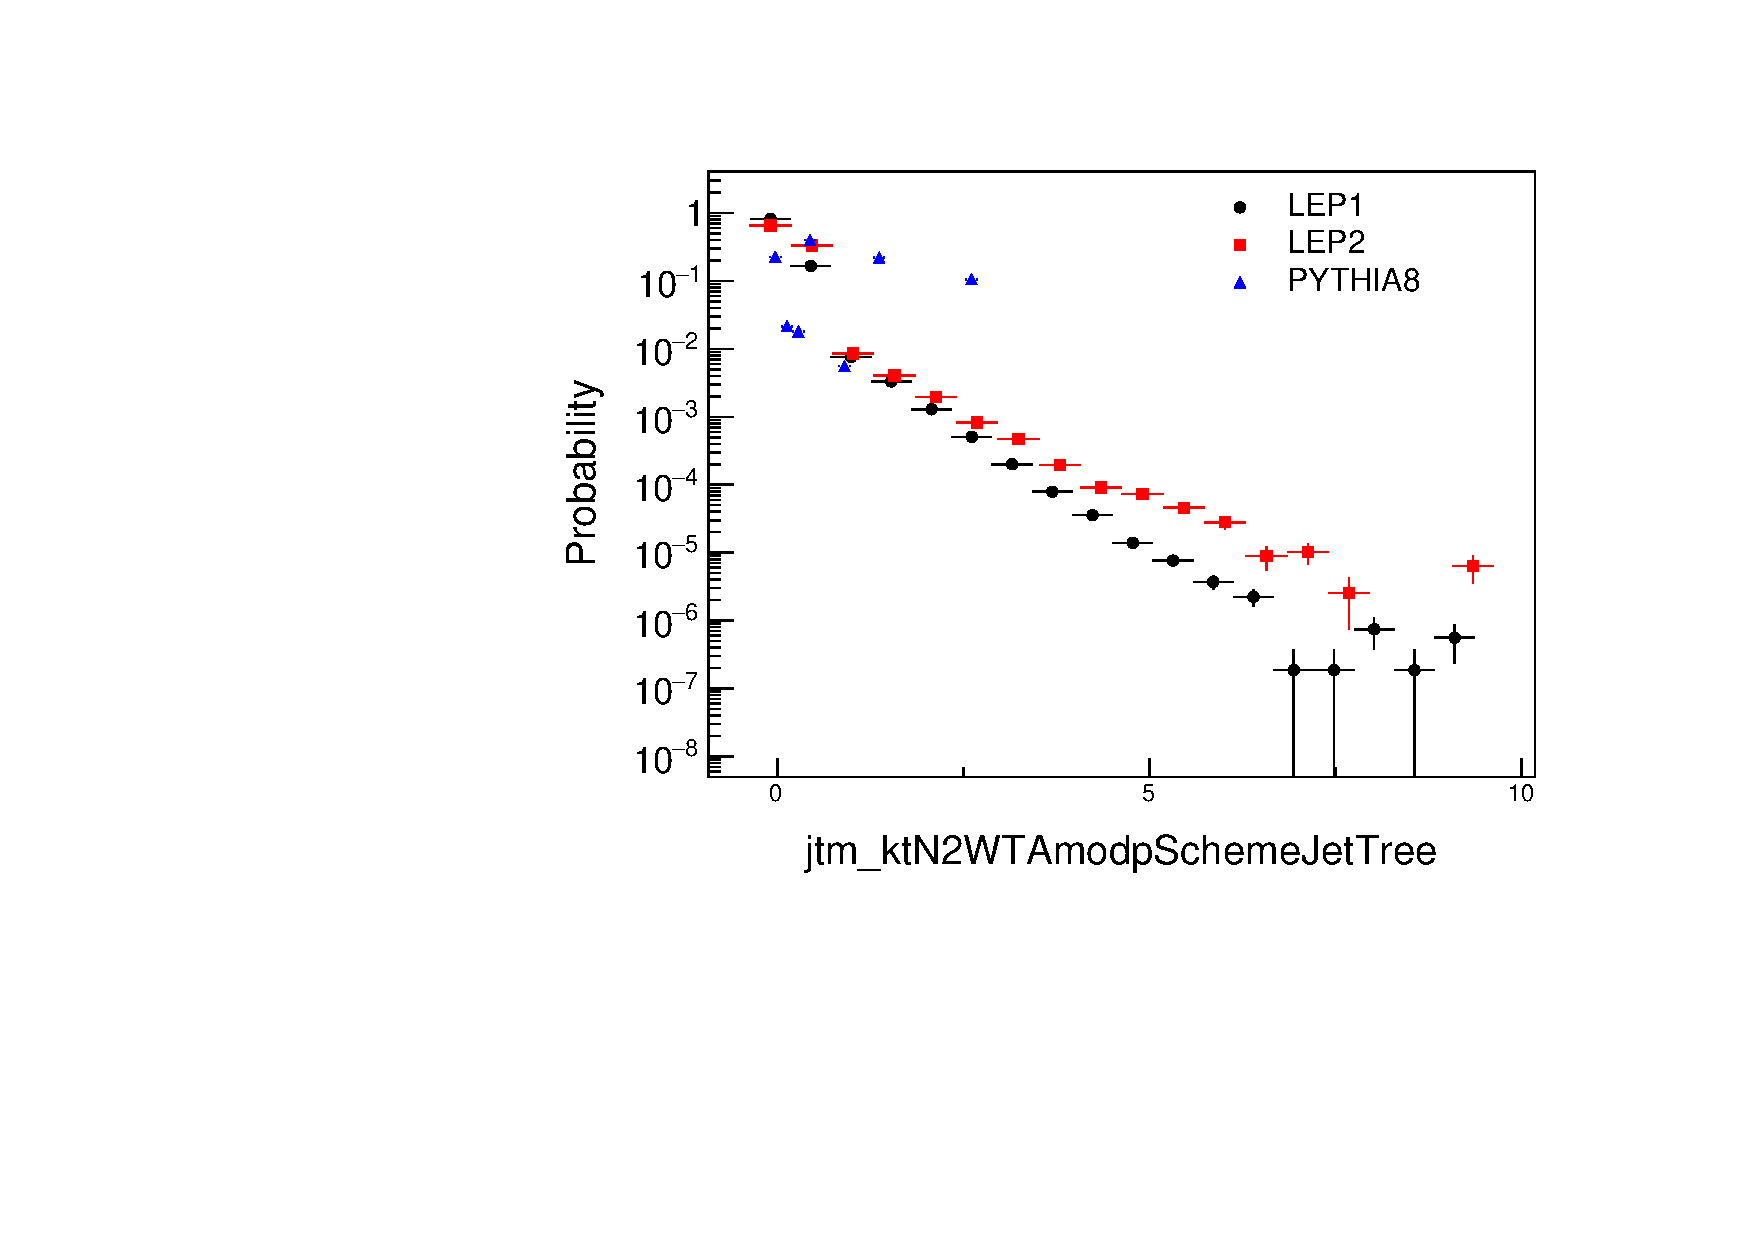
\includegraphics[width=.25\textwidth]{images/DQC/NoCut/jtm_ktN2WTAmodpSchemeJetTree.pdf}}\hfill
\subfloat{\label{sfig:h}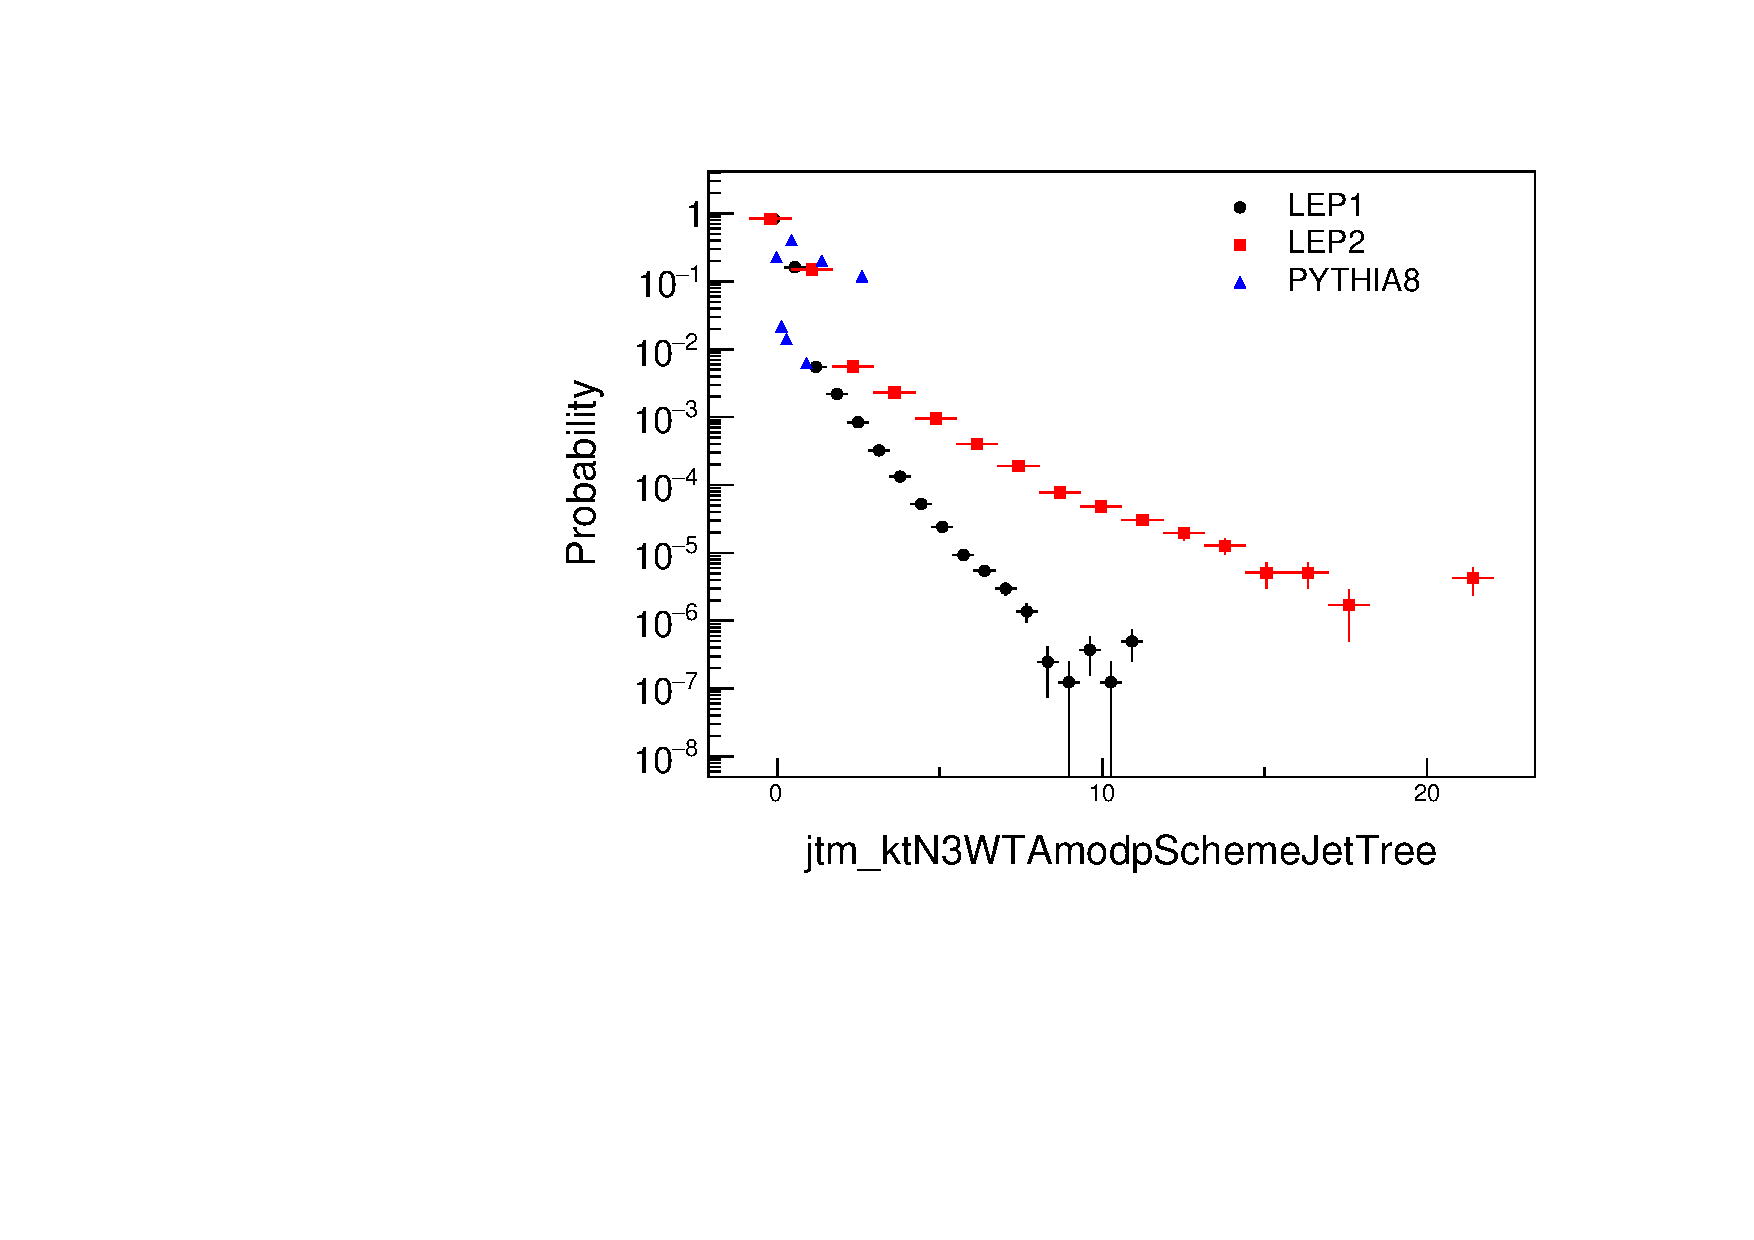
\includegraphics[width=.25\textwidth]{images/DQC/NoCut/jtm_ktN3WTAmodpSchemeJetTree.pdf}}\hfill
\caption{Raw Data: LEP1, LEP2, Pythia8 no cuts. Jet mass distributions. Top row: anti-$k_t$, left to right: $R=0.4$, $E$ scheme; $R=0.8$, $E$ scheme; $R=0.4$, WTA mod p scheme; $R=0.8$, WTA mod p scheme. Bottom row: $k_t$, left to right: $N=2$, $E$ scheme; $N=3$, $E$ scheme; $N=2$, WTA mod p scheme; $N=3$; WTA mod p scheme.}  
\end{figure}

\begin{figure}[H]
\centering
\subfloat{\label{sfig:a}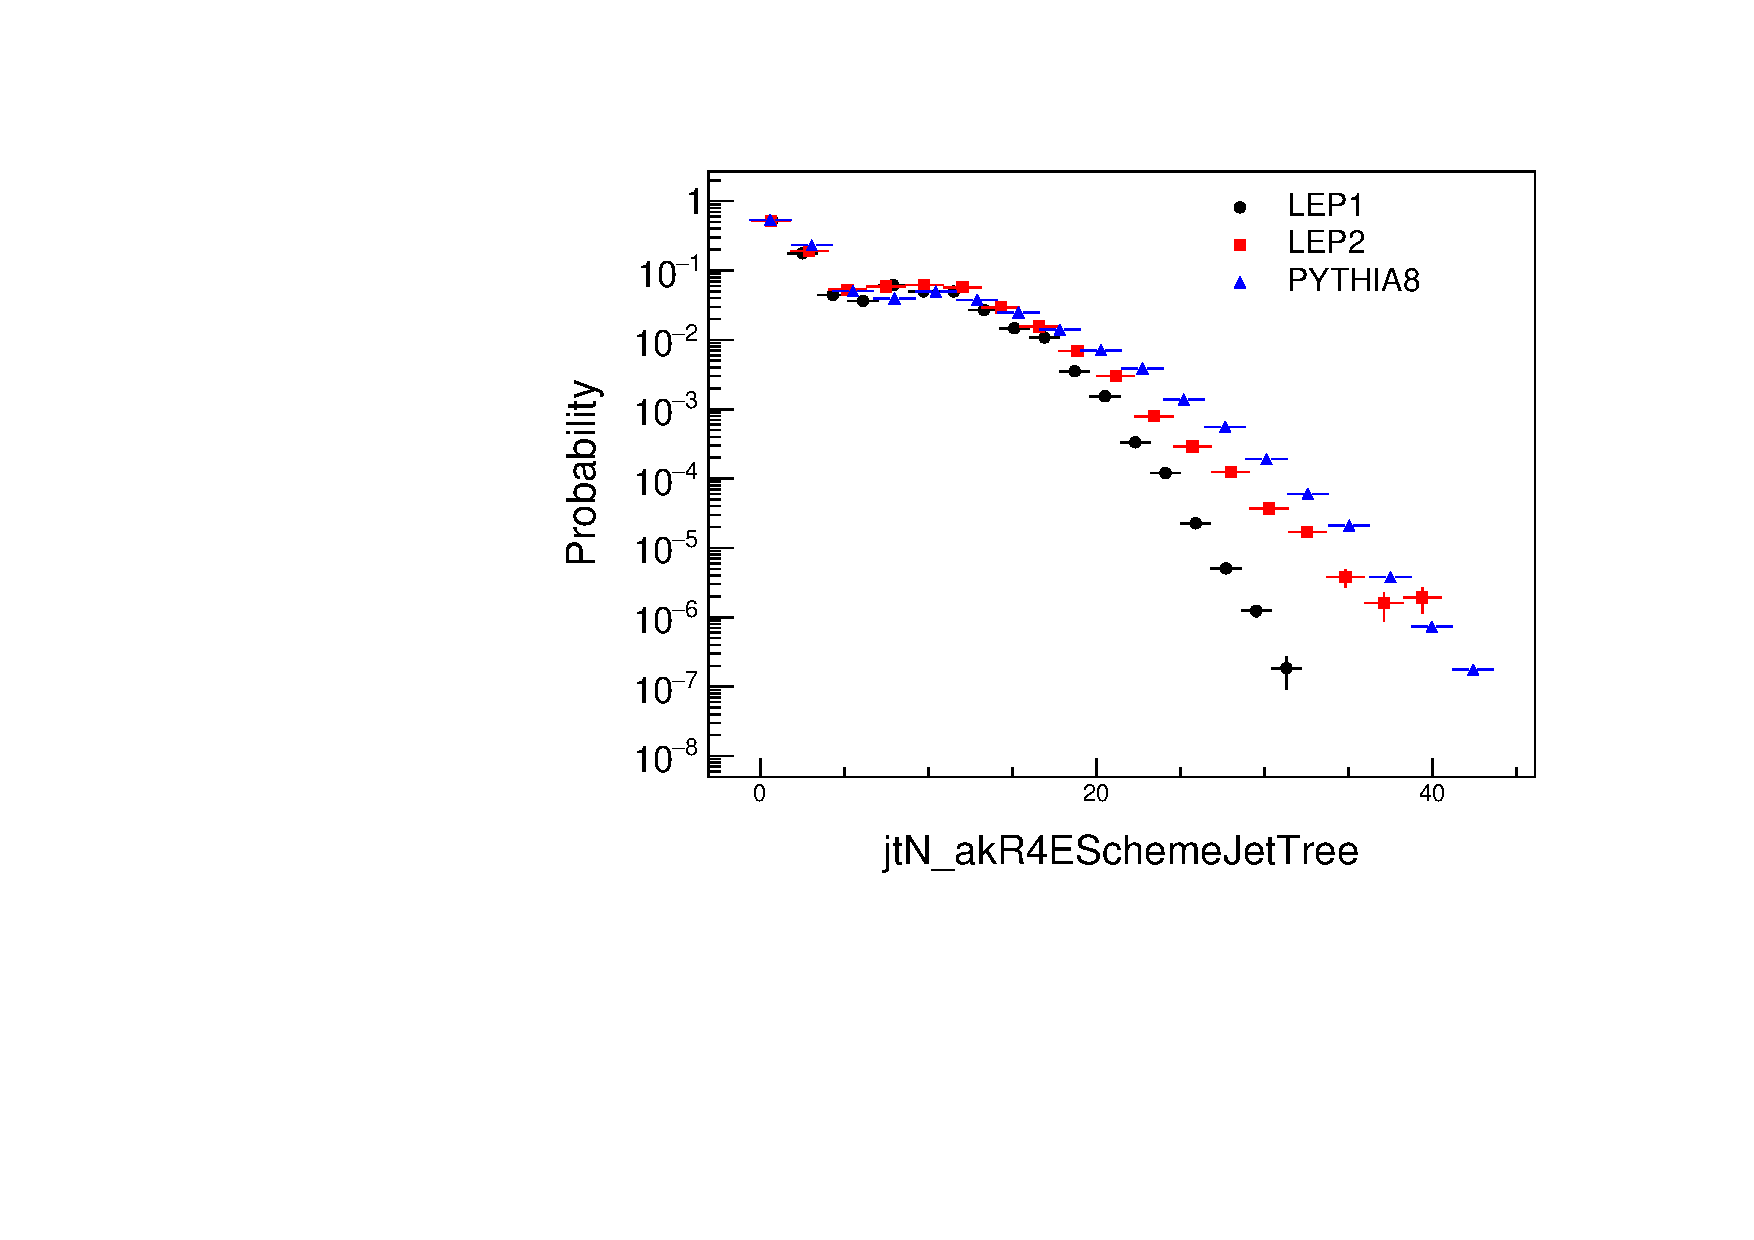
\includegraphics[width=.25\textwidth]{images/DQC/NoCut/jtN_akR4ESchemeJetTree.pdf}}\hfill
\subfloat{\label{sfig:b}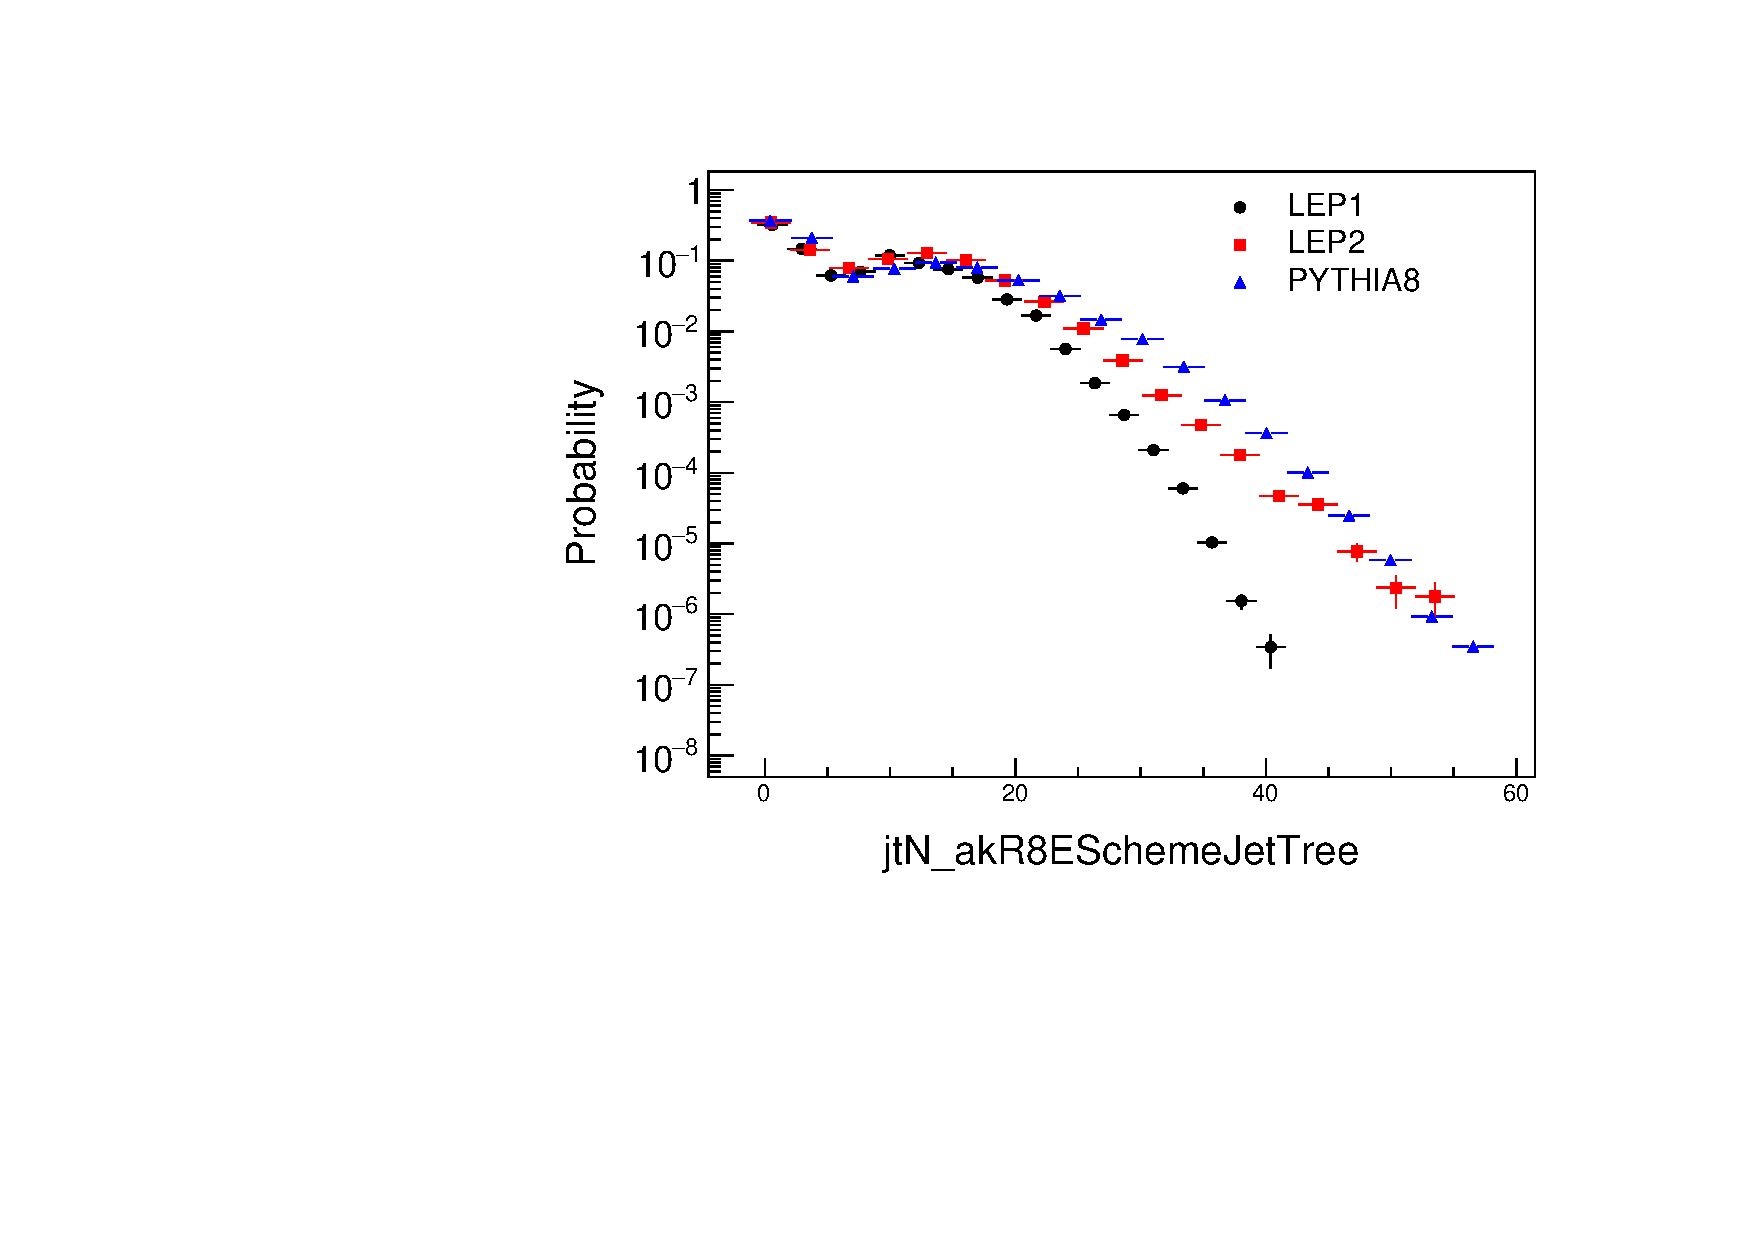
\includegraphics[width=.25\textwidth]{images/DQC/NoCut/jtN_akR8ESchemeJetTree.pdf}}\hfill
\subfloat{\label{sfig:c}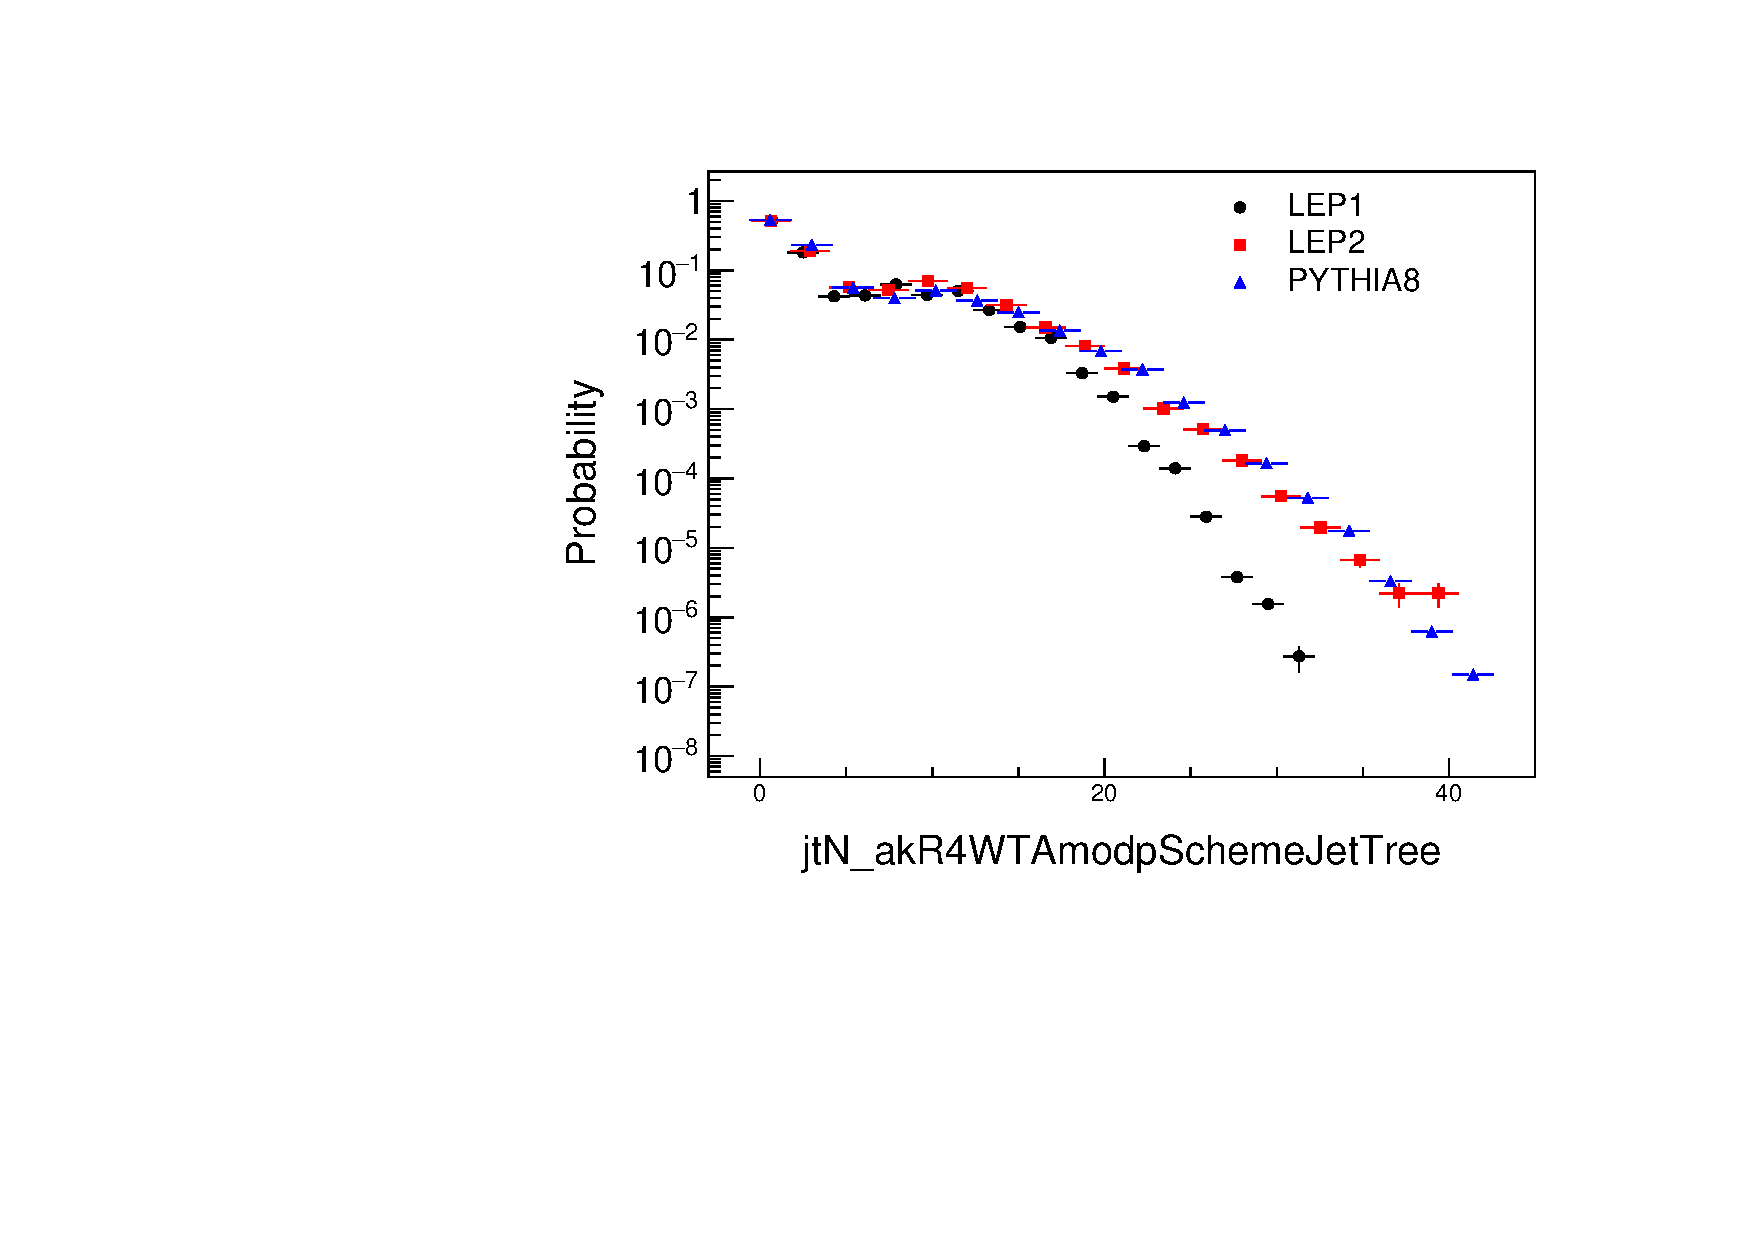
\includegraphics[width=.25\textwidth]{images/DQC/NoCut/jtN_akR4WTAmodpSchemeJetTree.pdf}}\hfill
\subfloat{\label{sfig:d}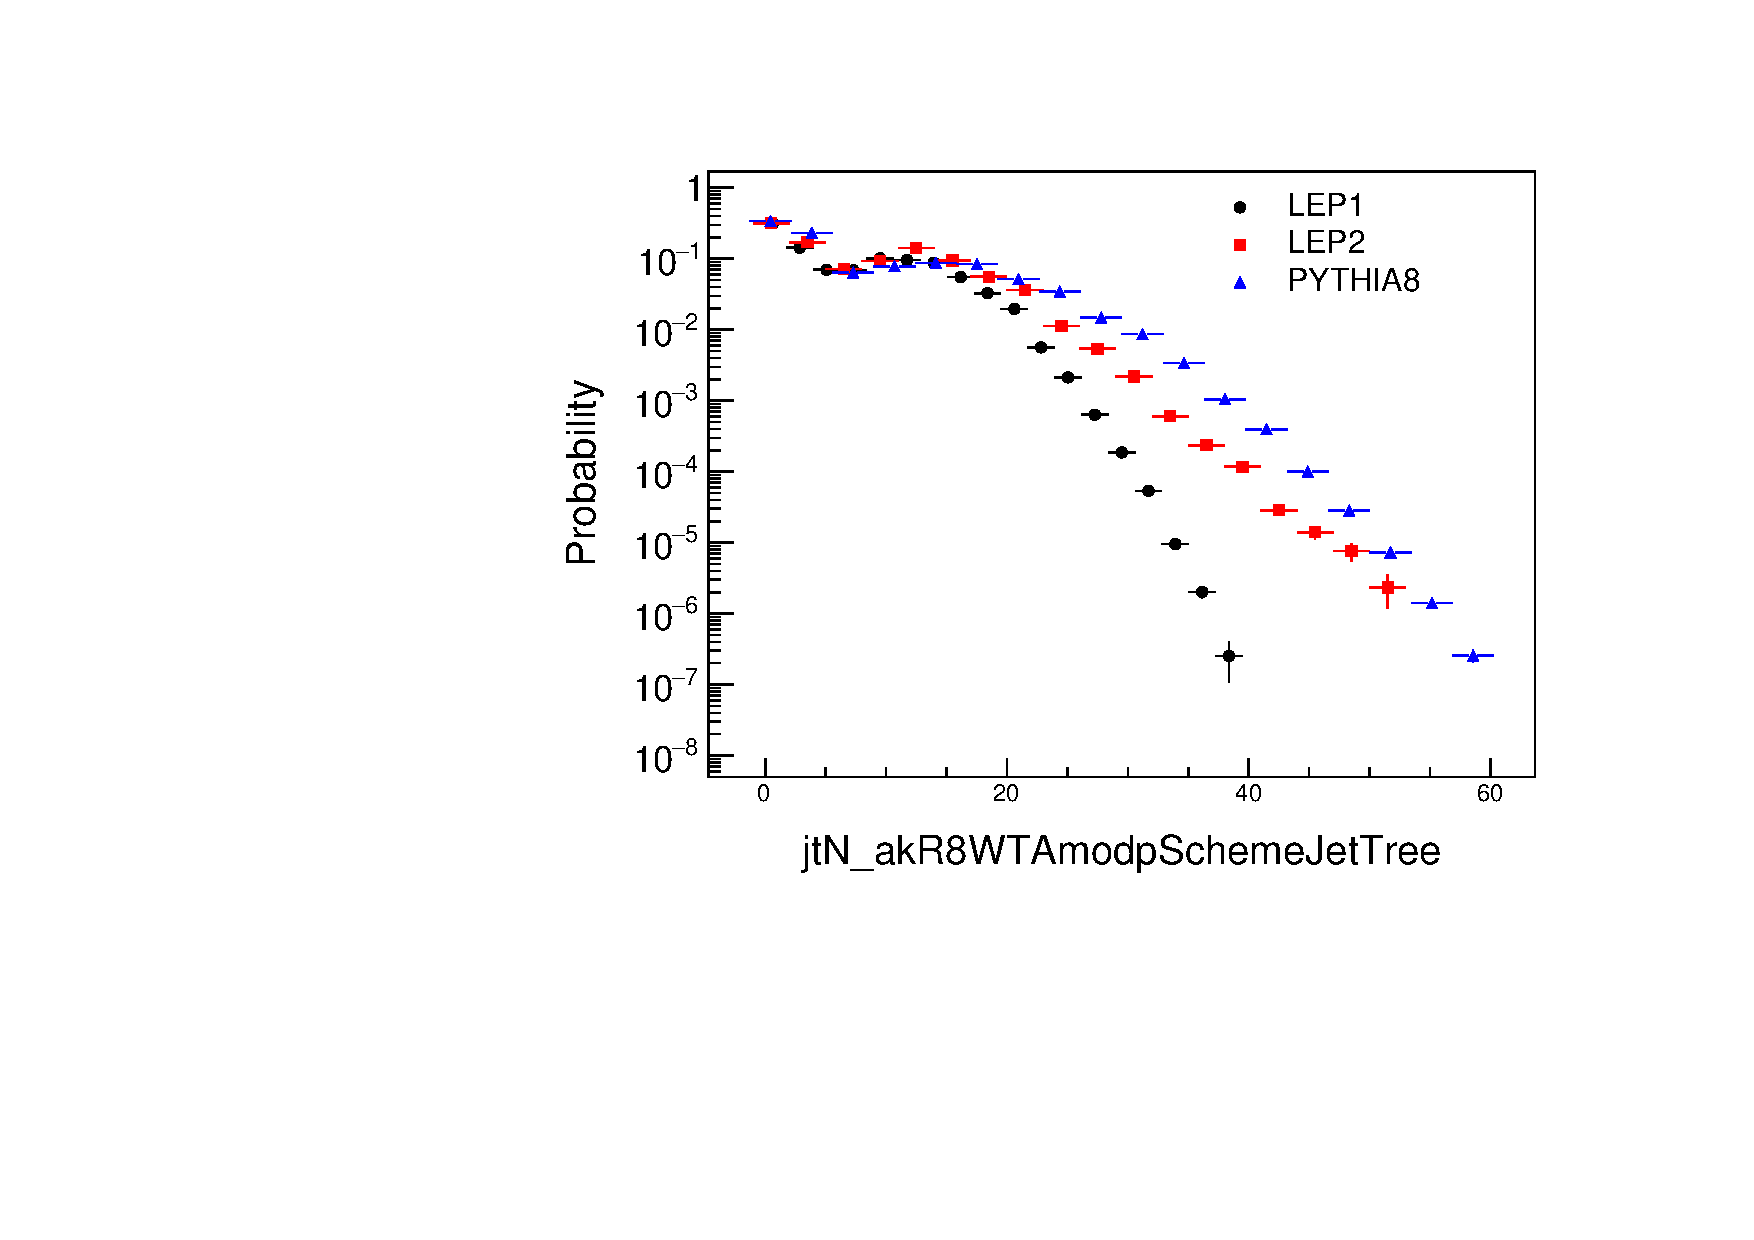
\includegraphics[width=.25\textwidth]{images/DQC/NoCut/jtN_akR8WTAmodpSchemeJetTree.pdf}}\hfill %row end
\subfloat{\label{sfig:e}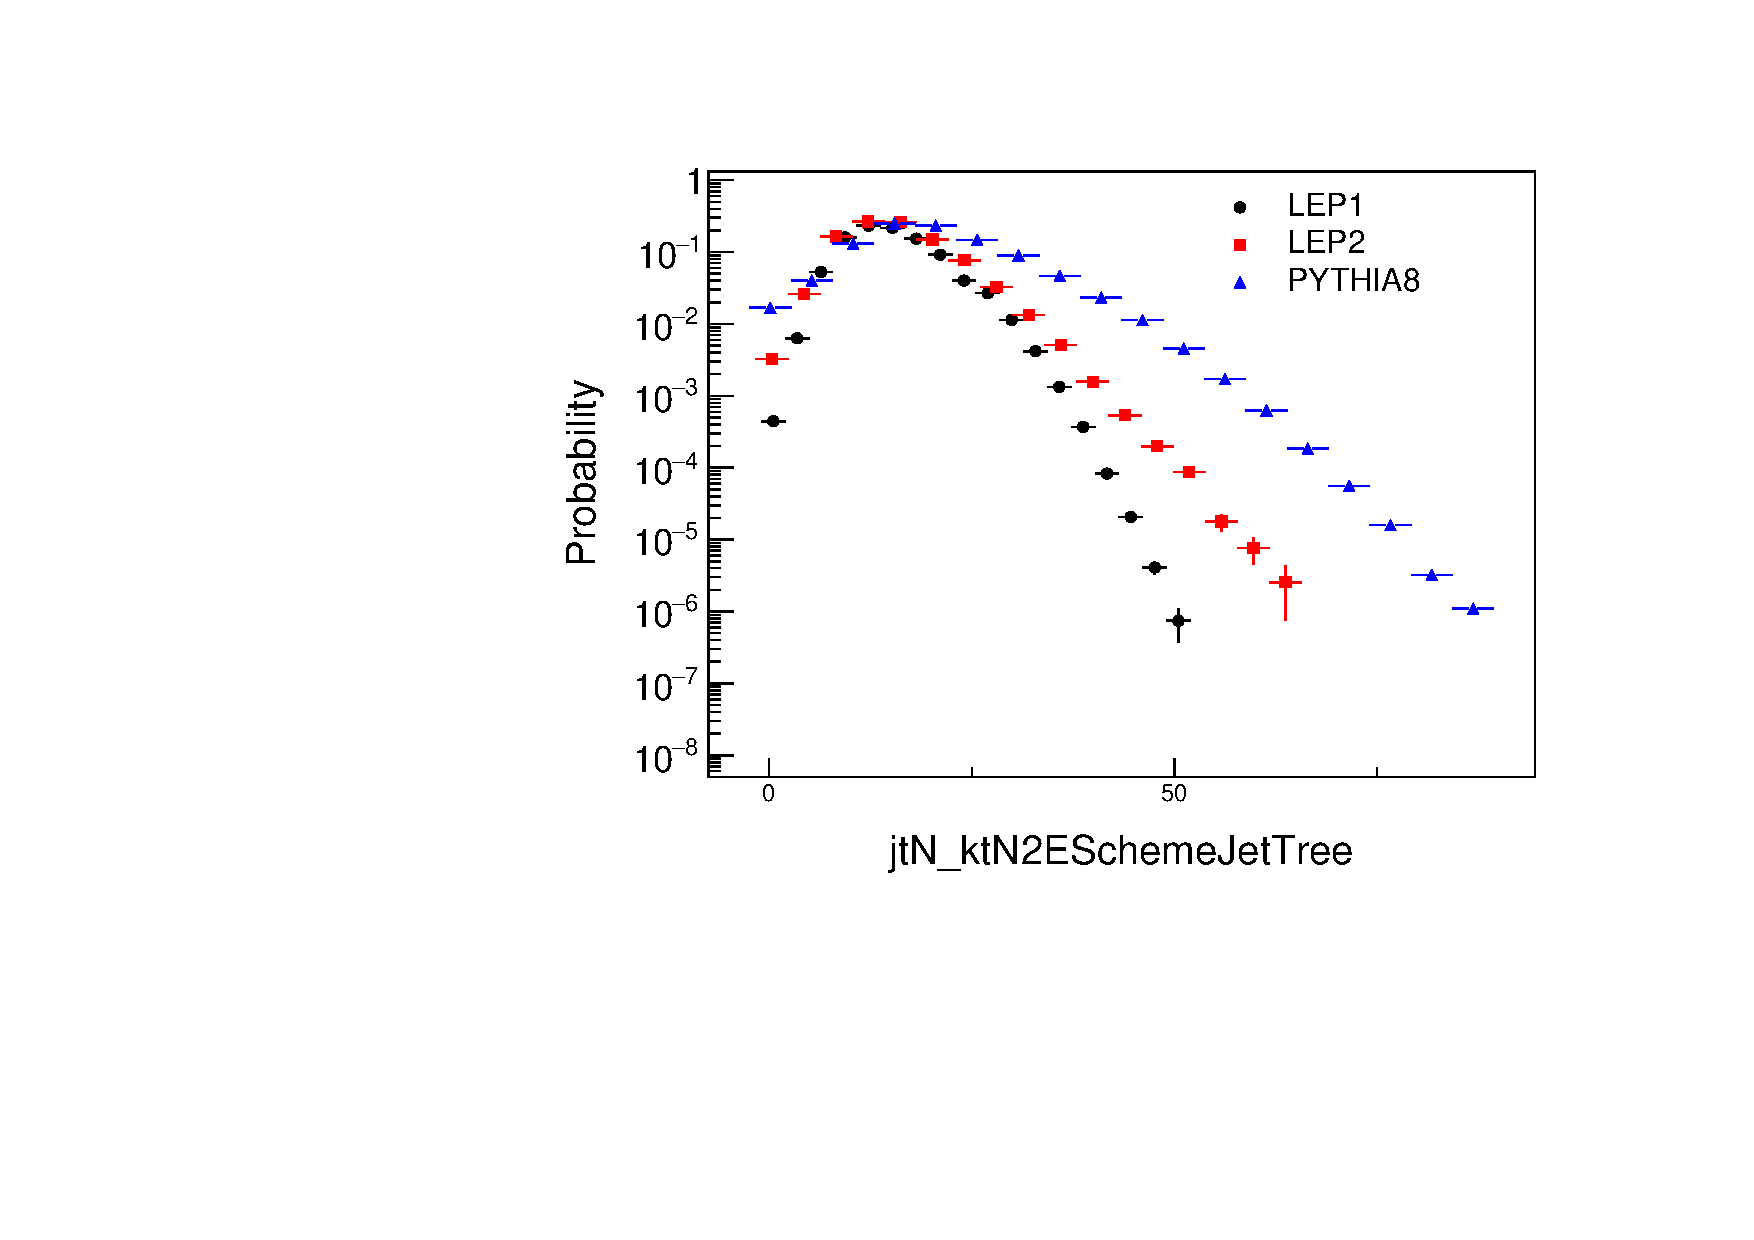
\includegraphics[width=.25\textwidth]{images/DQC/NoCut/jtN_ktN2ESchemeJetTree.pdf}}\hfill
\subfloat{\label{sfig:f}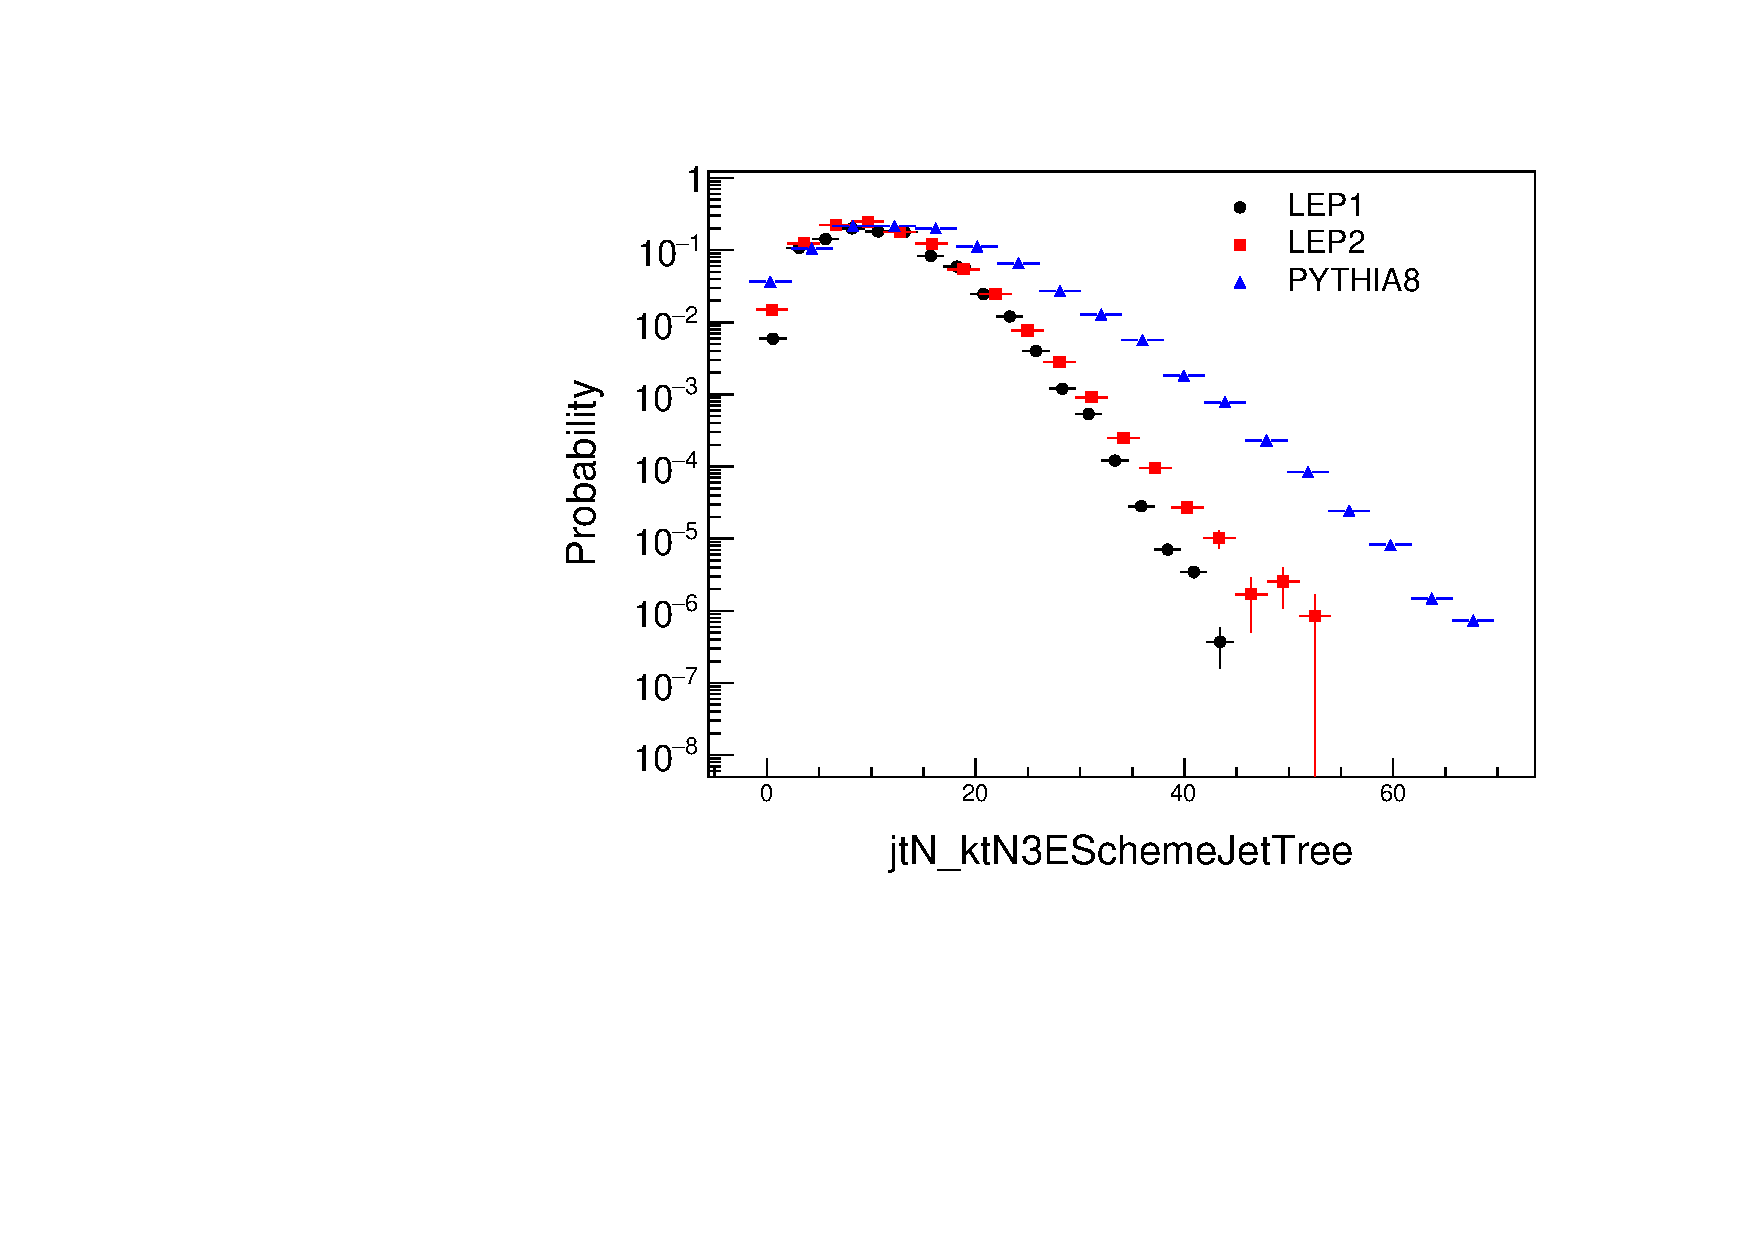
\includegraphics[width=.25\textwidth]{images/DQC/NoCut/jtN_ktN3ESchemeJetTree.pdf}}\hfill
\subfloat{\label{sfig:g}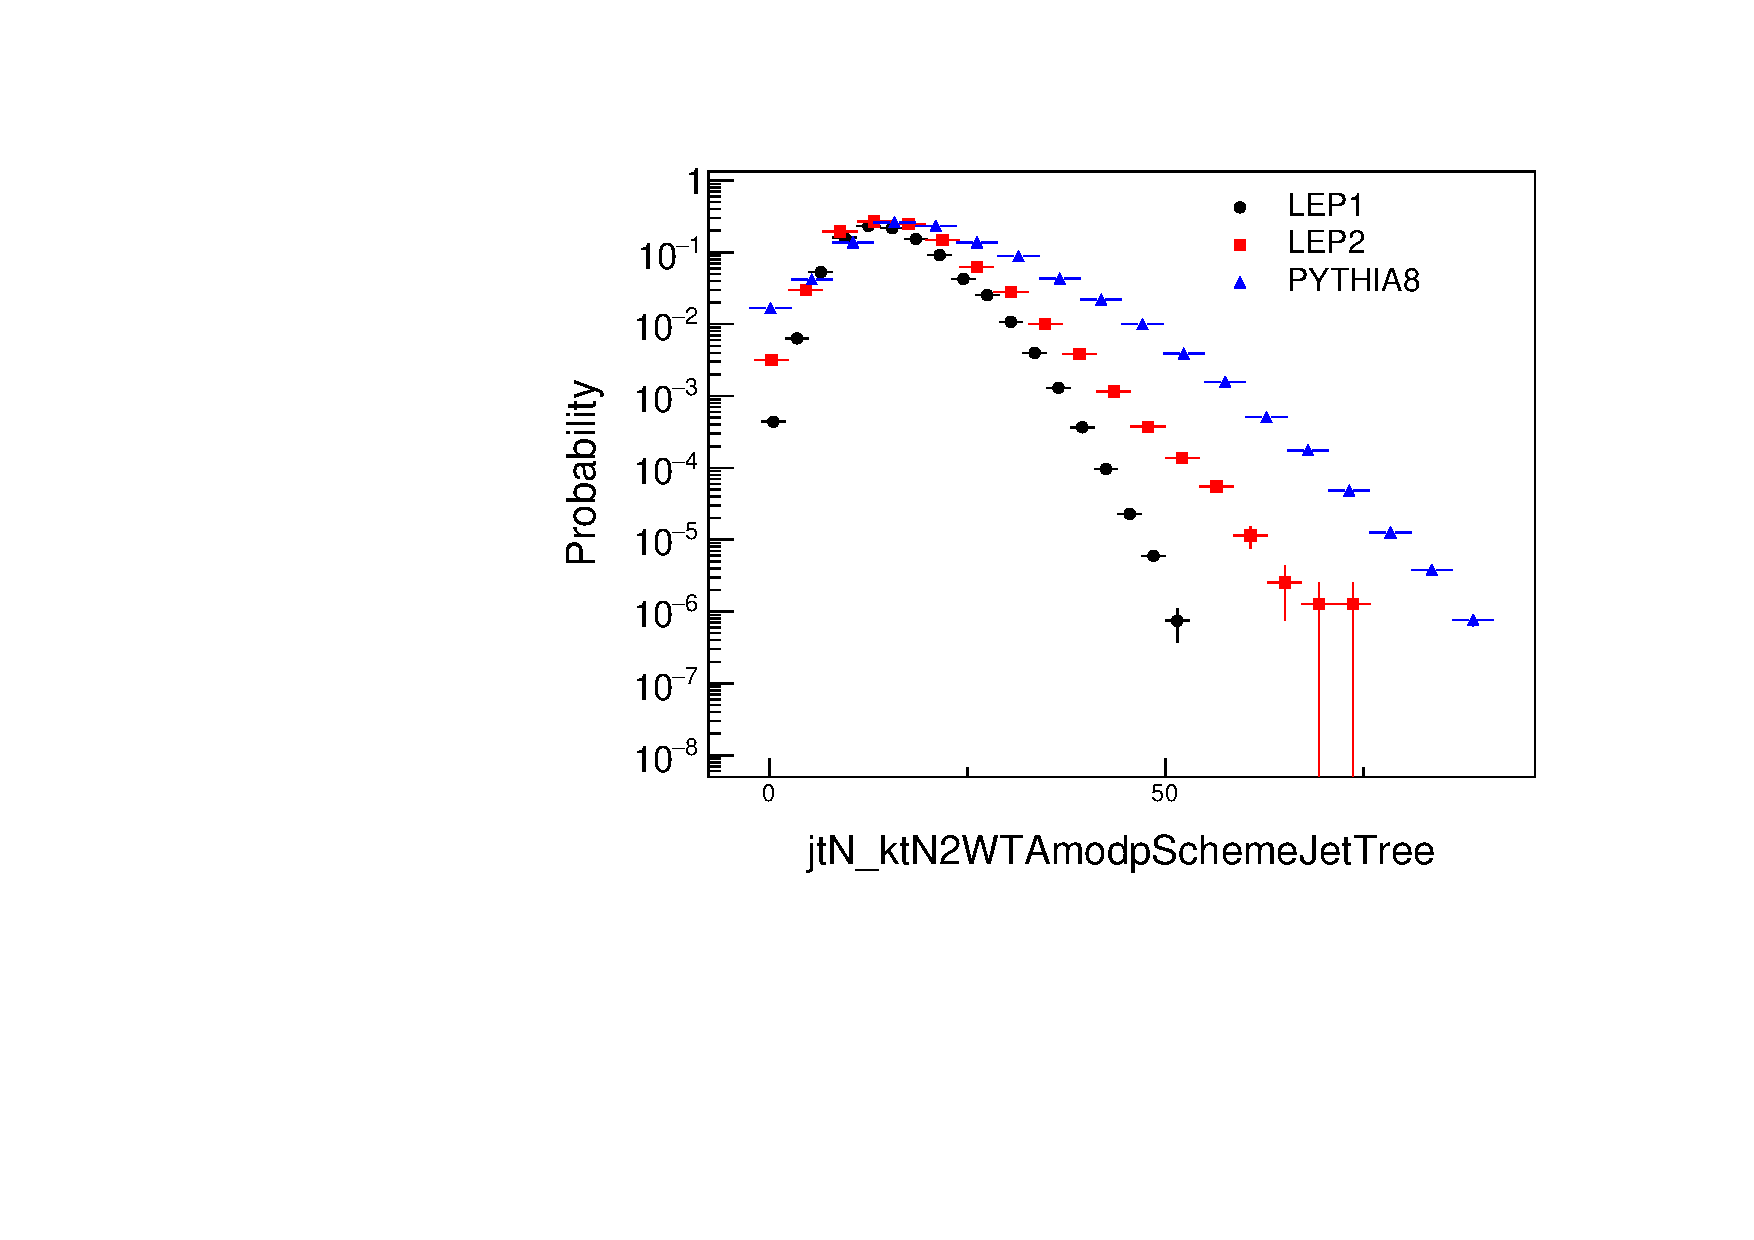
\includegraphics[width=.25\textwidth]{images/DQC/NoCut/jtN_ktN2WTAmodpSchemeJetTree.pdf}}\hfill
\subfloat{\label{sfig:h}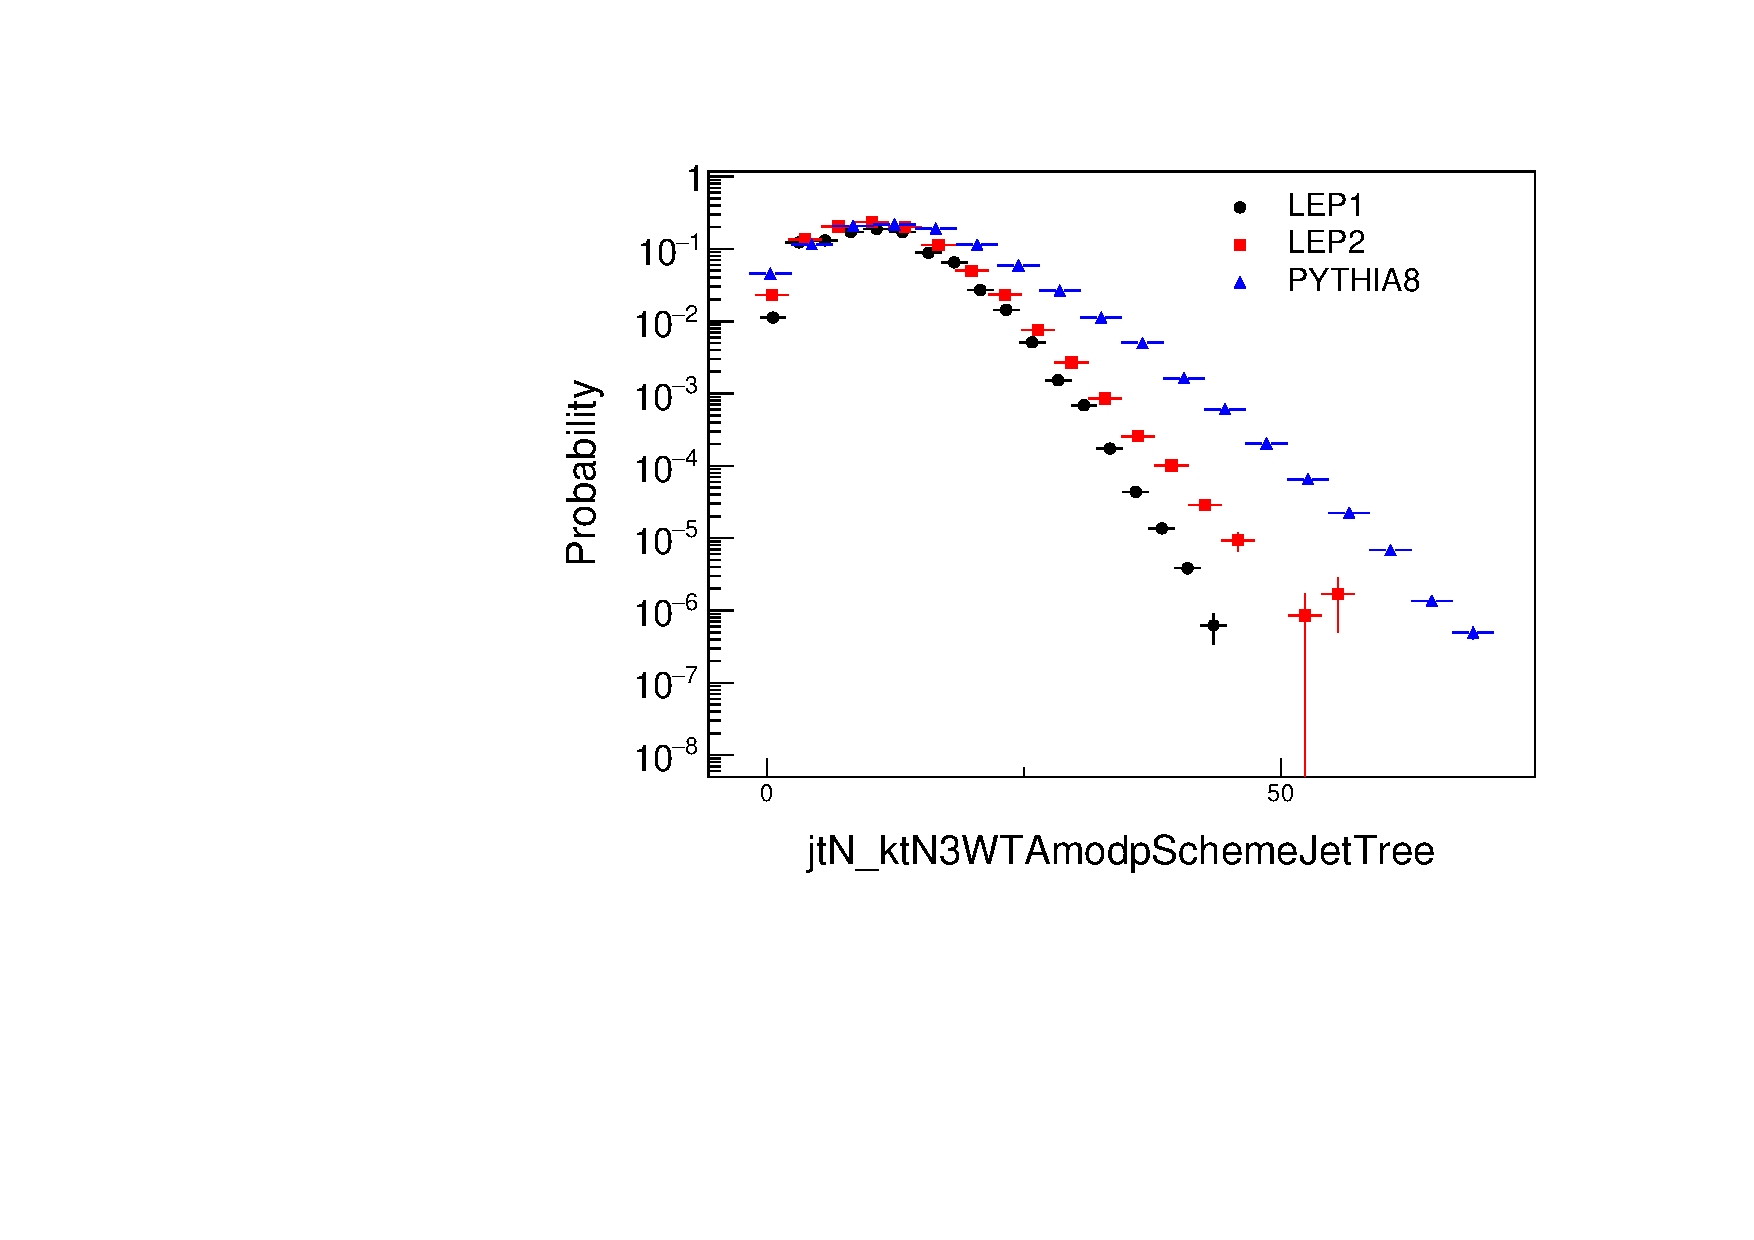
\includegraphics[width=.25\textwidth]{images/DQC/NoCut/jtN_ktN3WTAmodpSchemeJetTree.pdf}}\hfill
\caption{Raw Data: LEP1, LEP2, Pythia8 no cuts. Jet $N$ distributions. Top row: anti-$k_t$, left to right: $R=0.4$, $E$ scheme; $R=0.8$, $E$ scheme; $R=0.4$, WTA mod p scheme; $R=0.8$, WTA mod p scheme. Bottom row: $k_t$, left to right: $N=2$, $E$ scheme; $N=3$, $E$ scheme; $N=2$, WTA mod p scheme; $N=3$; WTA mod p scheme.}  
\end{figure} 

\begin{figure}[H]
\centering
\subfloat{\label{sfig:a}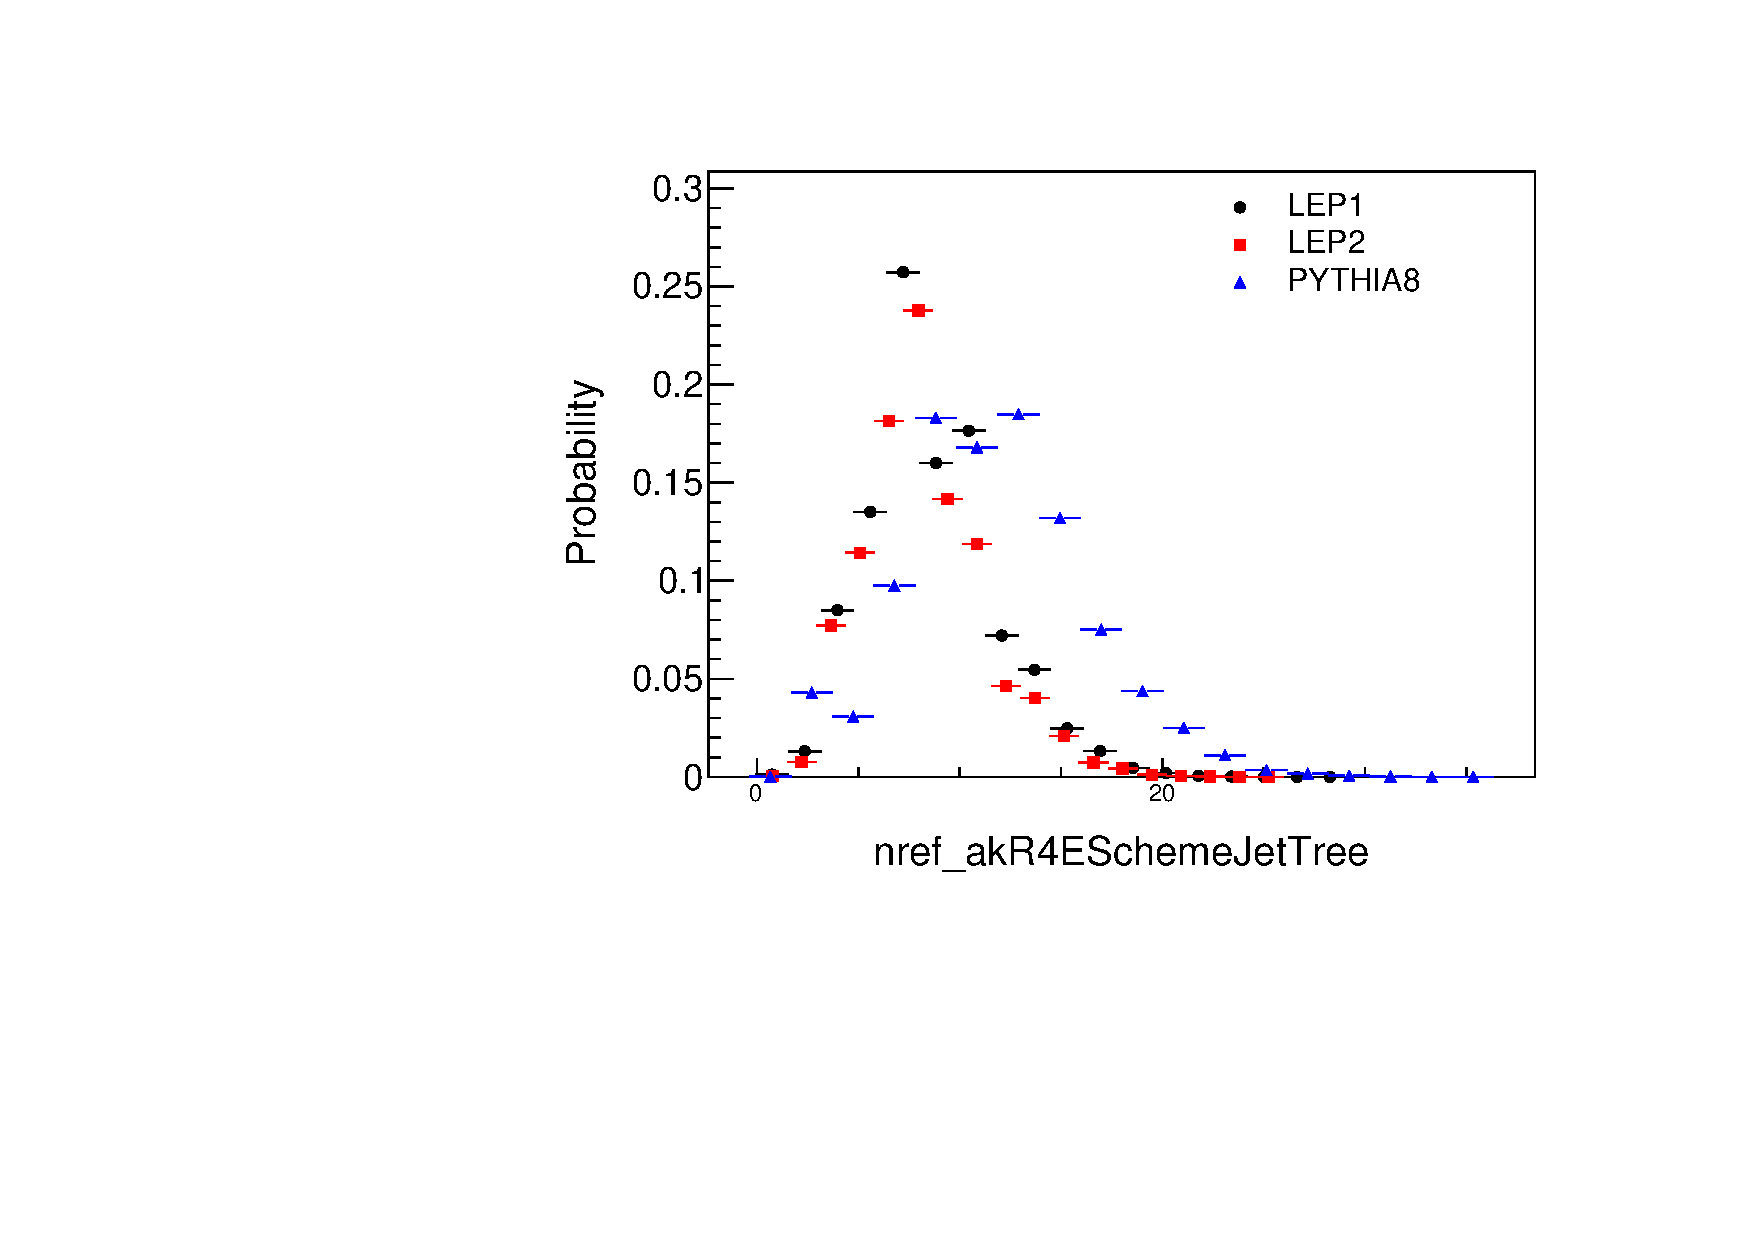
\includegraphics[width=.25\textwidth]{images/DQC/NoCut/nref_akR4ESchemeJetTree.pdf}}\hfill
\subfloat{\label{sfig:b}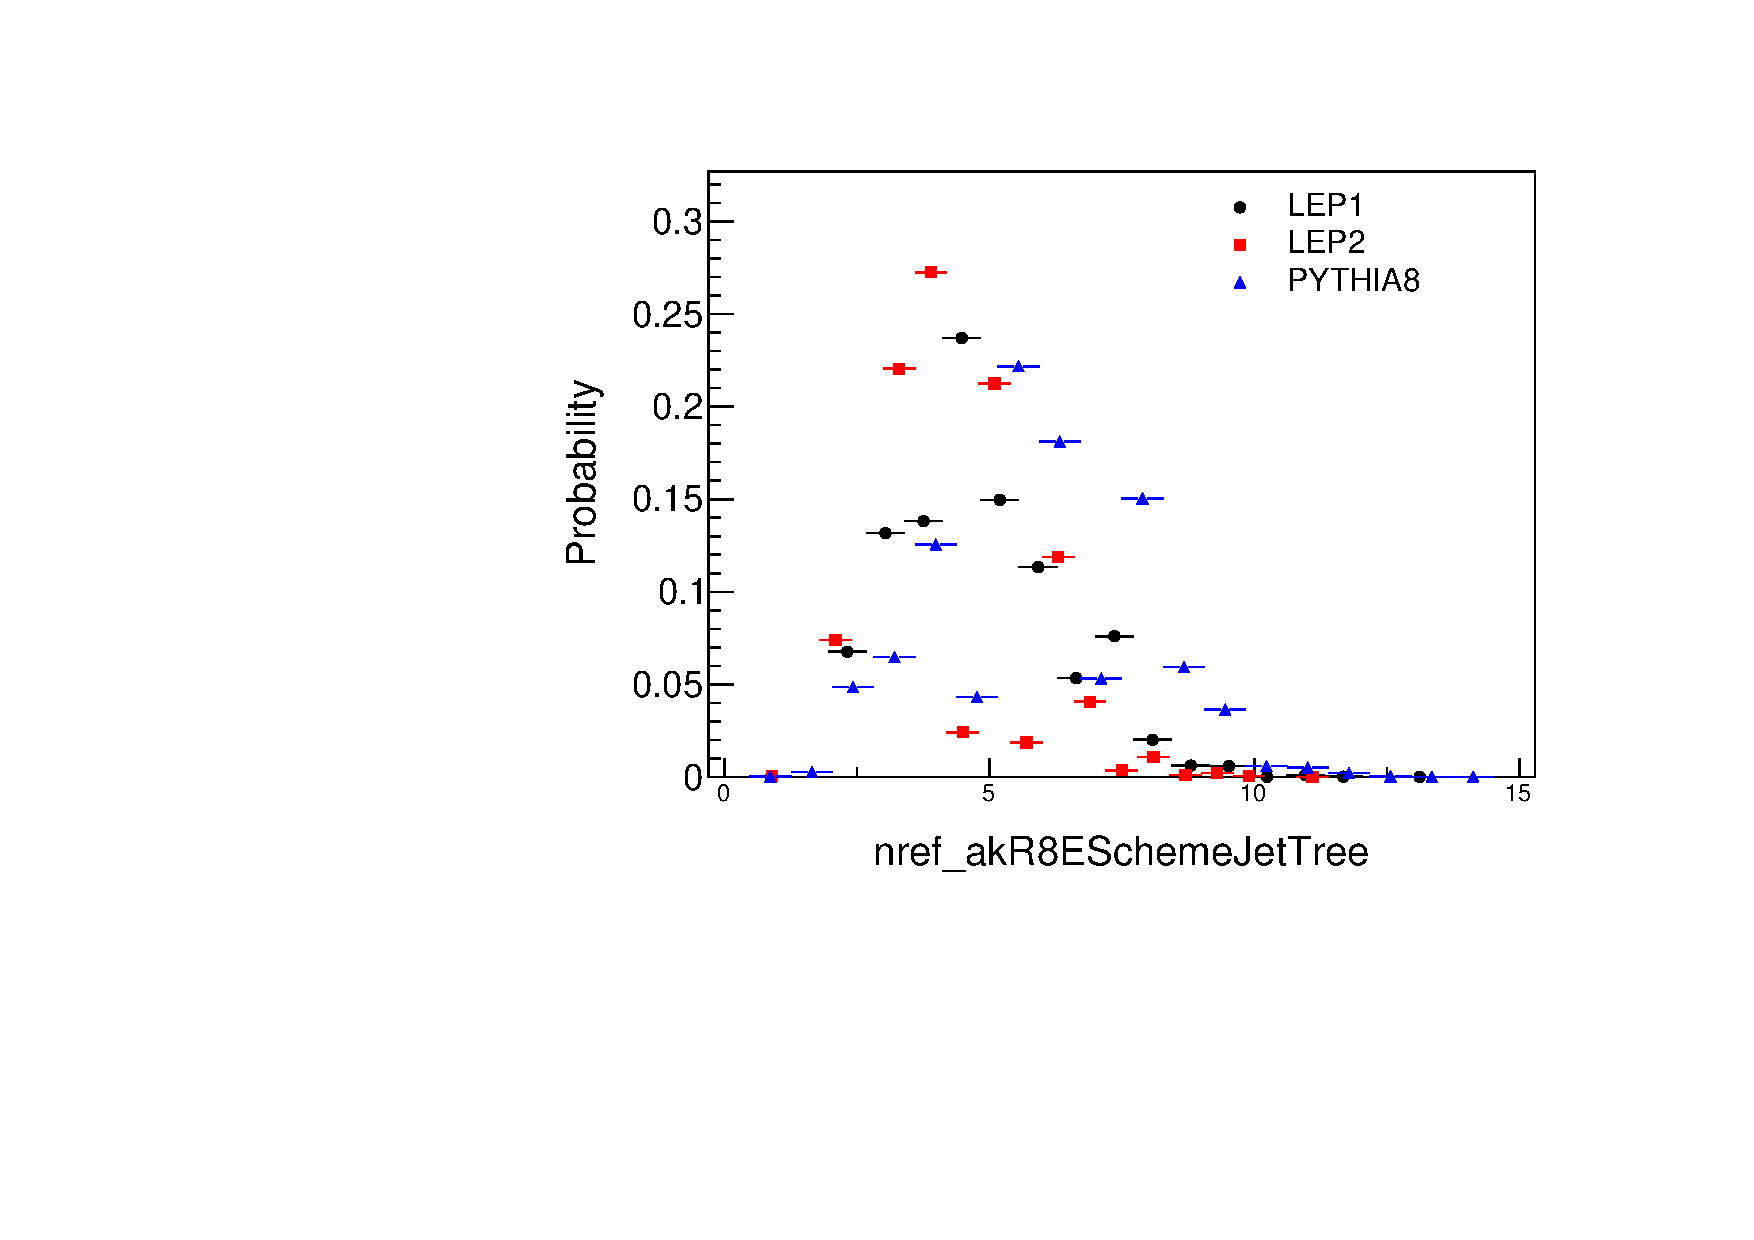
\includegraphics[width=.25\textwidth]{images/DQC/NoCut/nref_akR8ESchemeJetTree.pdf}}\hfill
\subfloat{\label{sfig:c}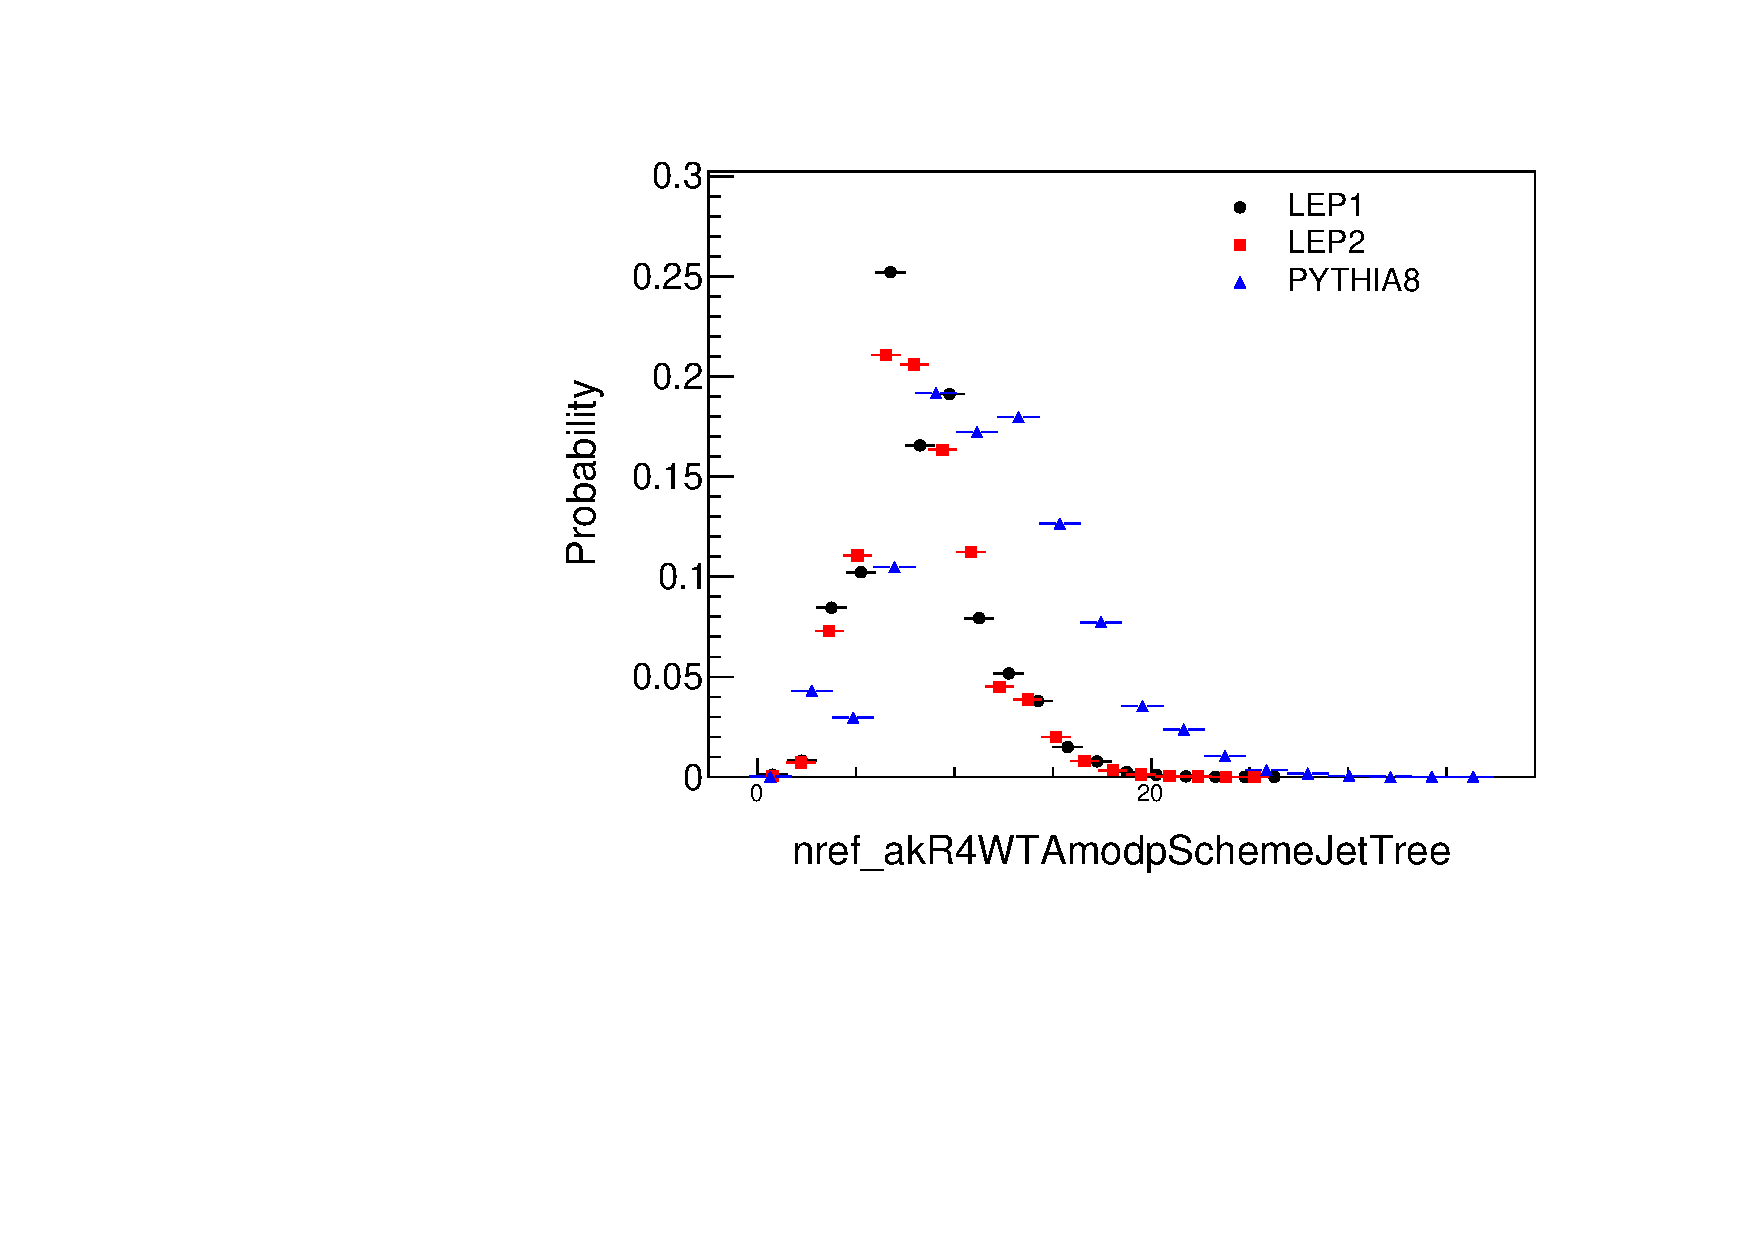
\includegraphics[width=.25\textwidth]{images/DQC/NoCut/nref_akR4WTAmodpSchemeJetTree.pdf}}\hfill
\subfloat{\label{sfig:d}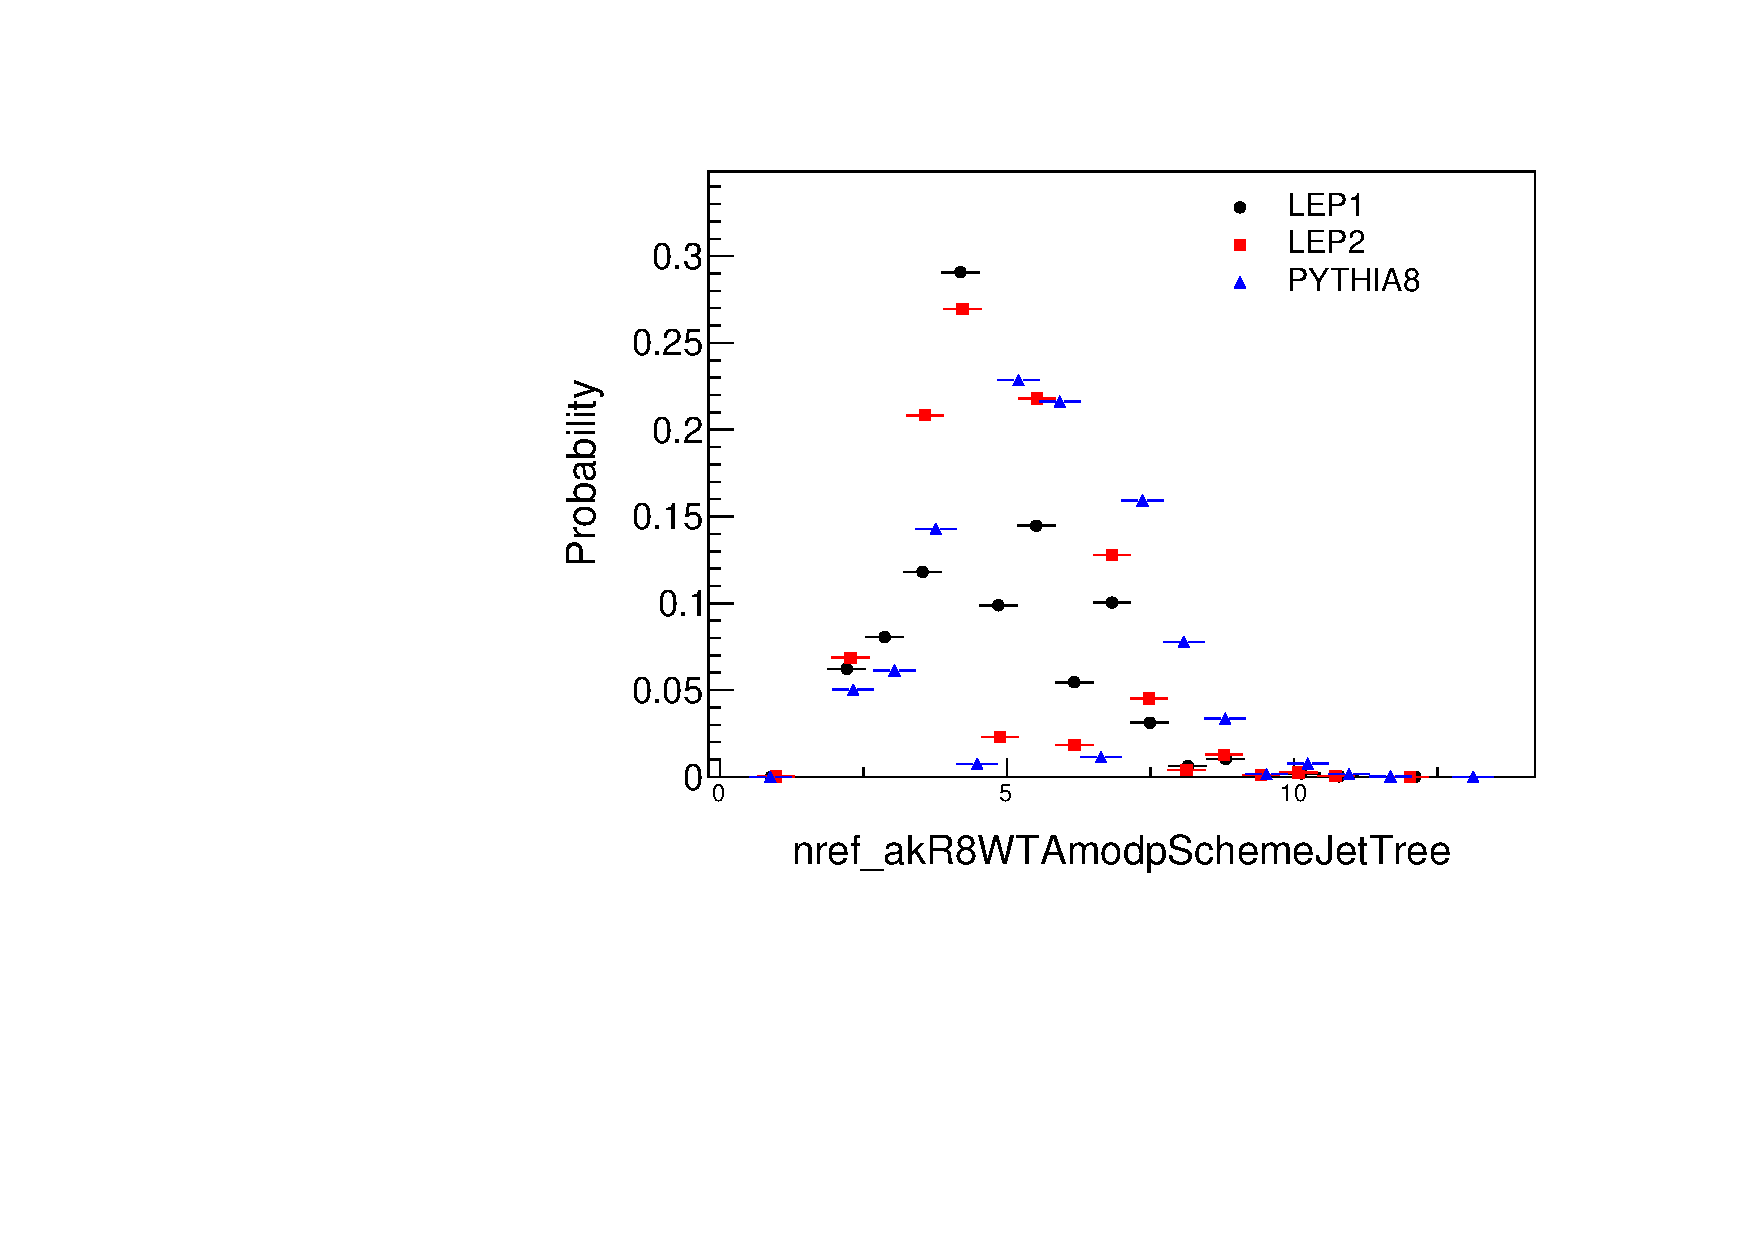
\includegraphics[width=.25\textwidth]{images/DQC/NoCut/nref_akR8WTAmodpSchemeJetTree.pdf}}\hfill %row end
\subfloat{\label{sfig:e}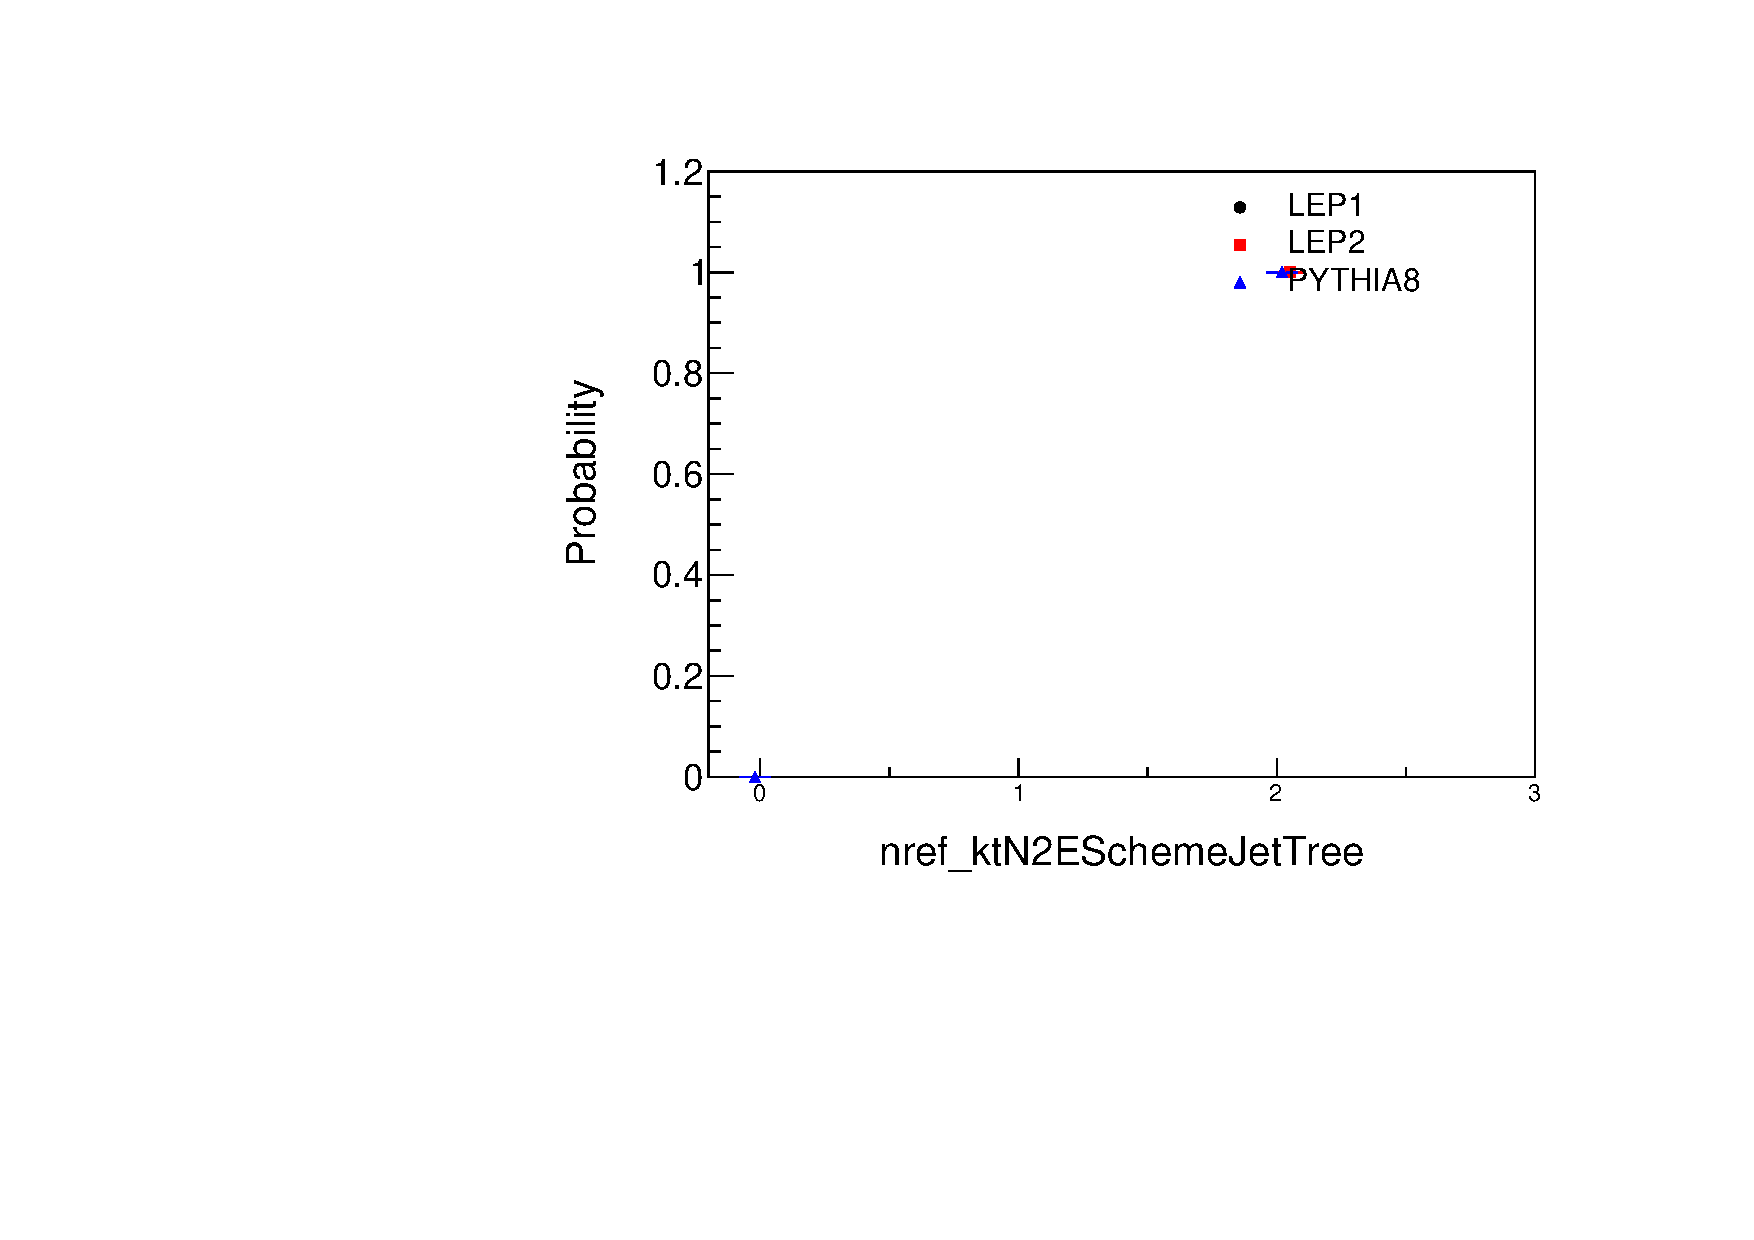
\includegraphics[width=.25\textwidth]{images/DQC/NoCut/nref_ktN2ESchemeJetTree.pdf}}\hfill
\subfloat{\label{sfig:f}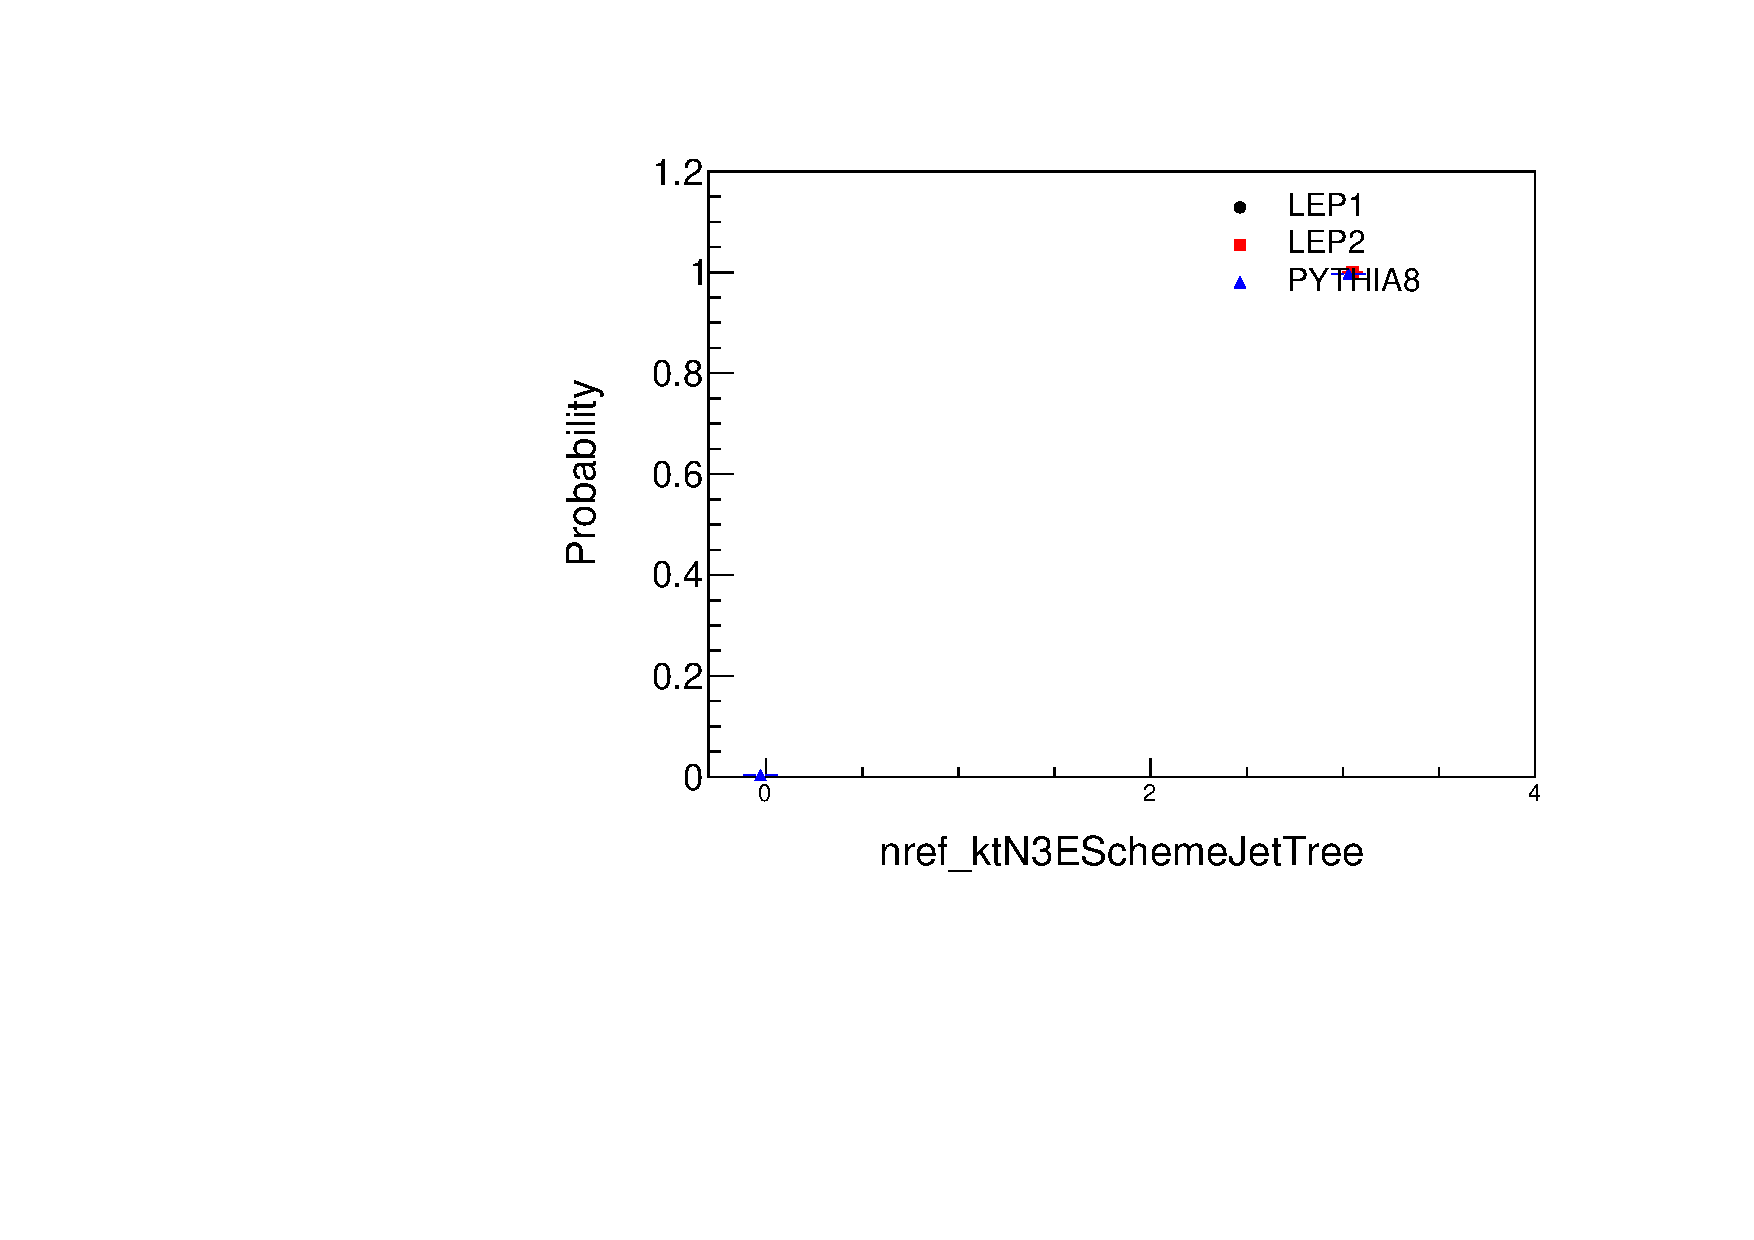
\includegraphics[width=.25\textwidth]{images/DQC/NoCut/nref_ktN3ESchemeJetTree.pdf}}\hfill
\subfloat{\label{sfig:g}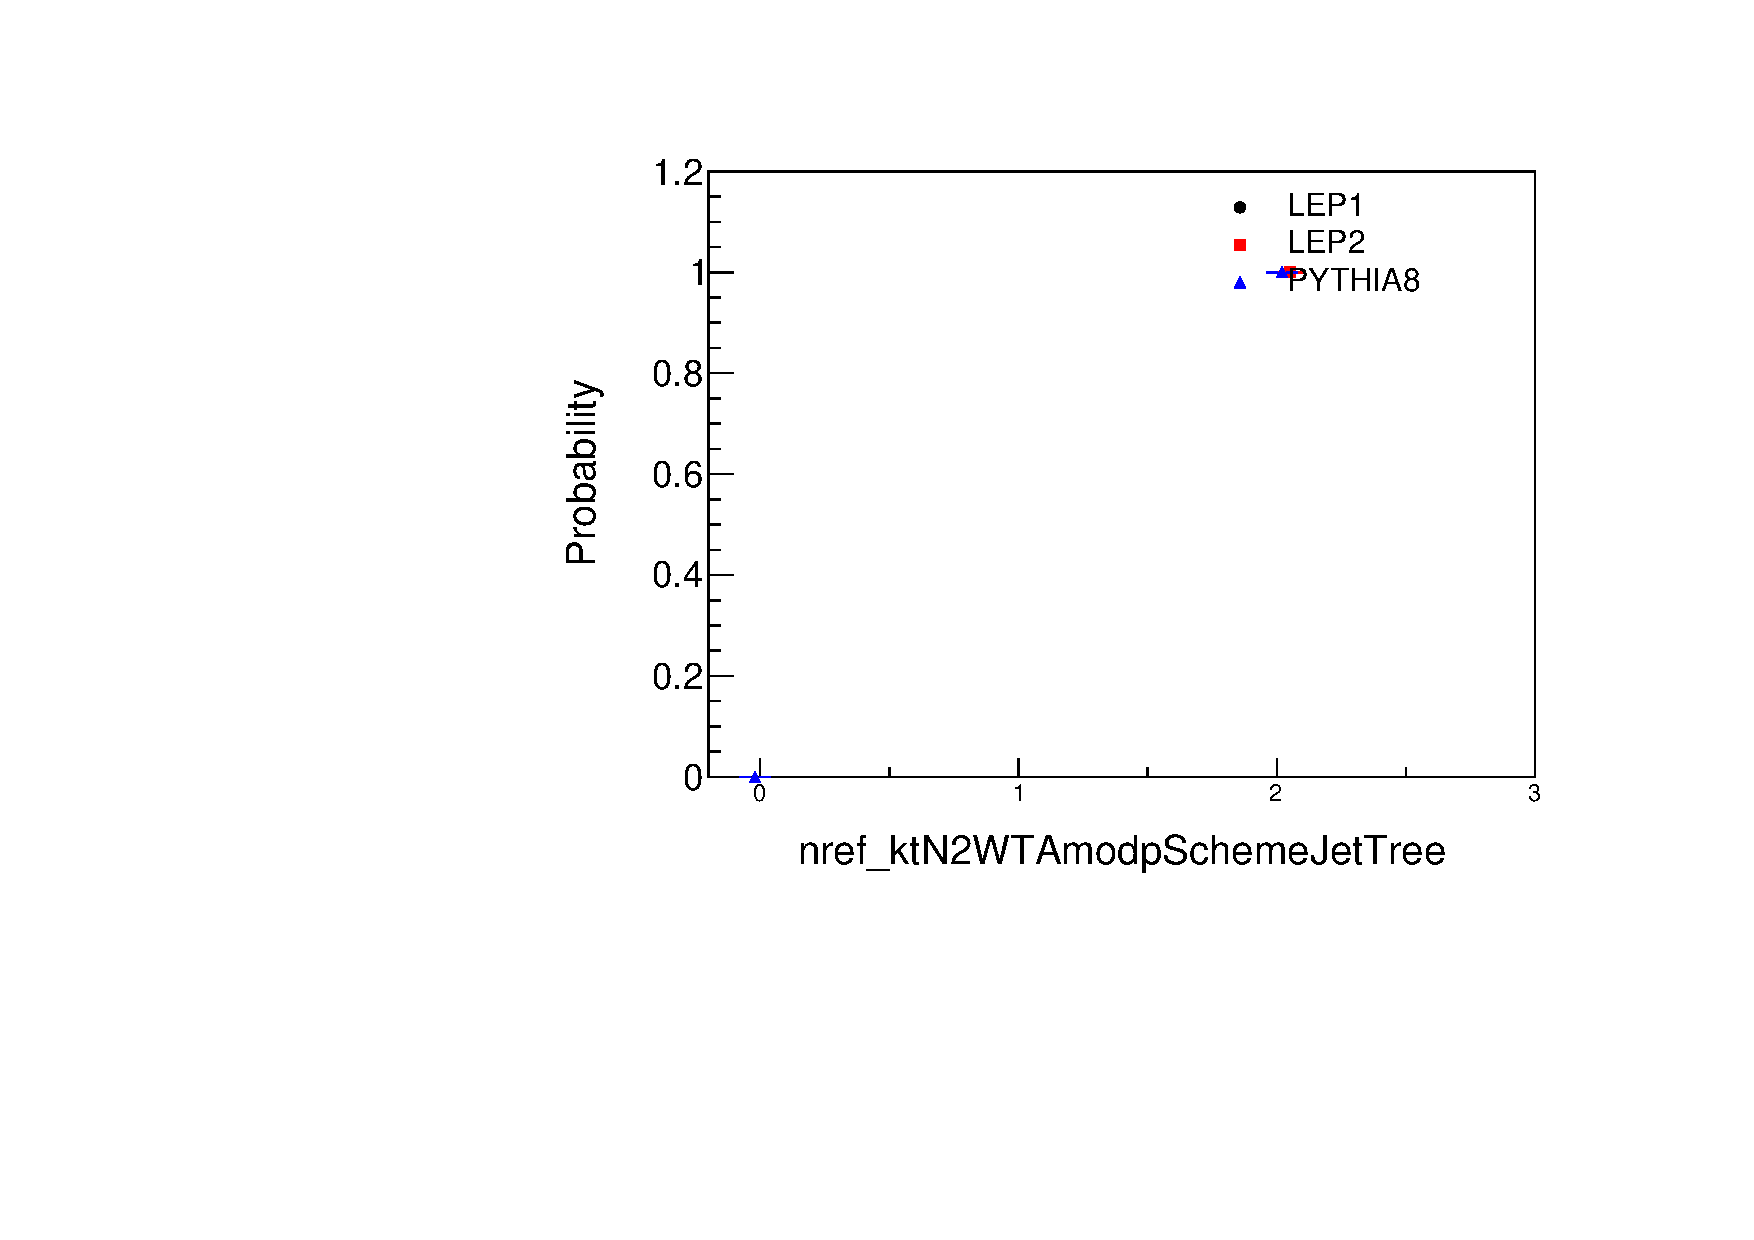
\includegraphics[width=.25\textwidth]{images/DQC/NoCut/nref_ktN2WTAmodpSchemeJetTree.pdf}}\hfill
\subfloat{\label{sfig:h}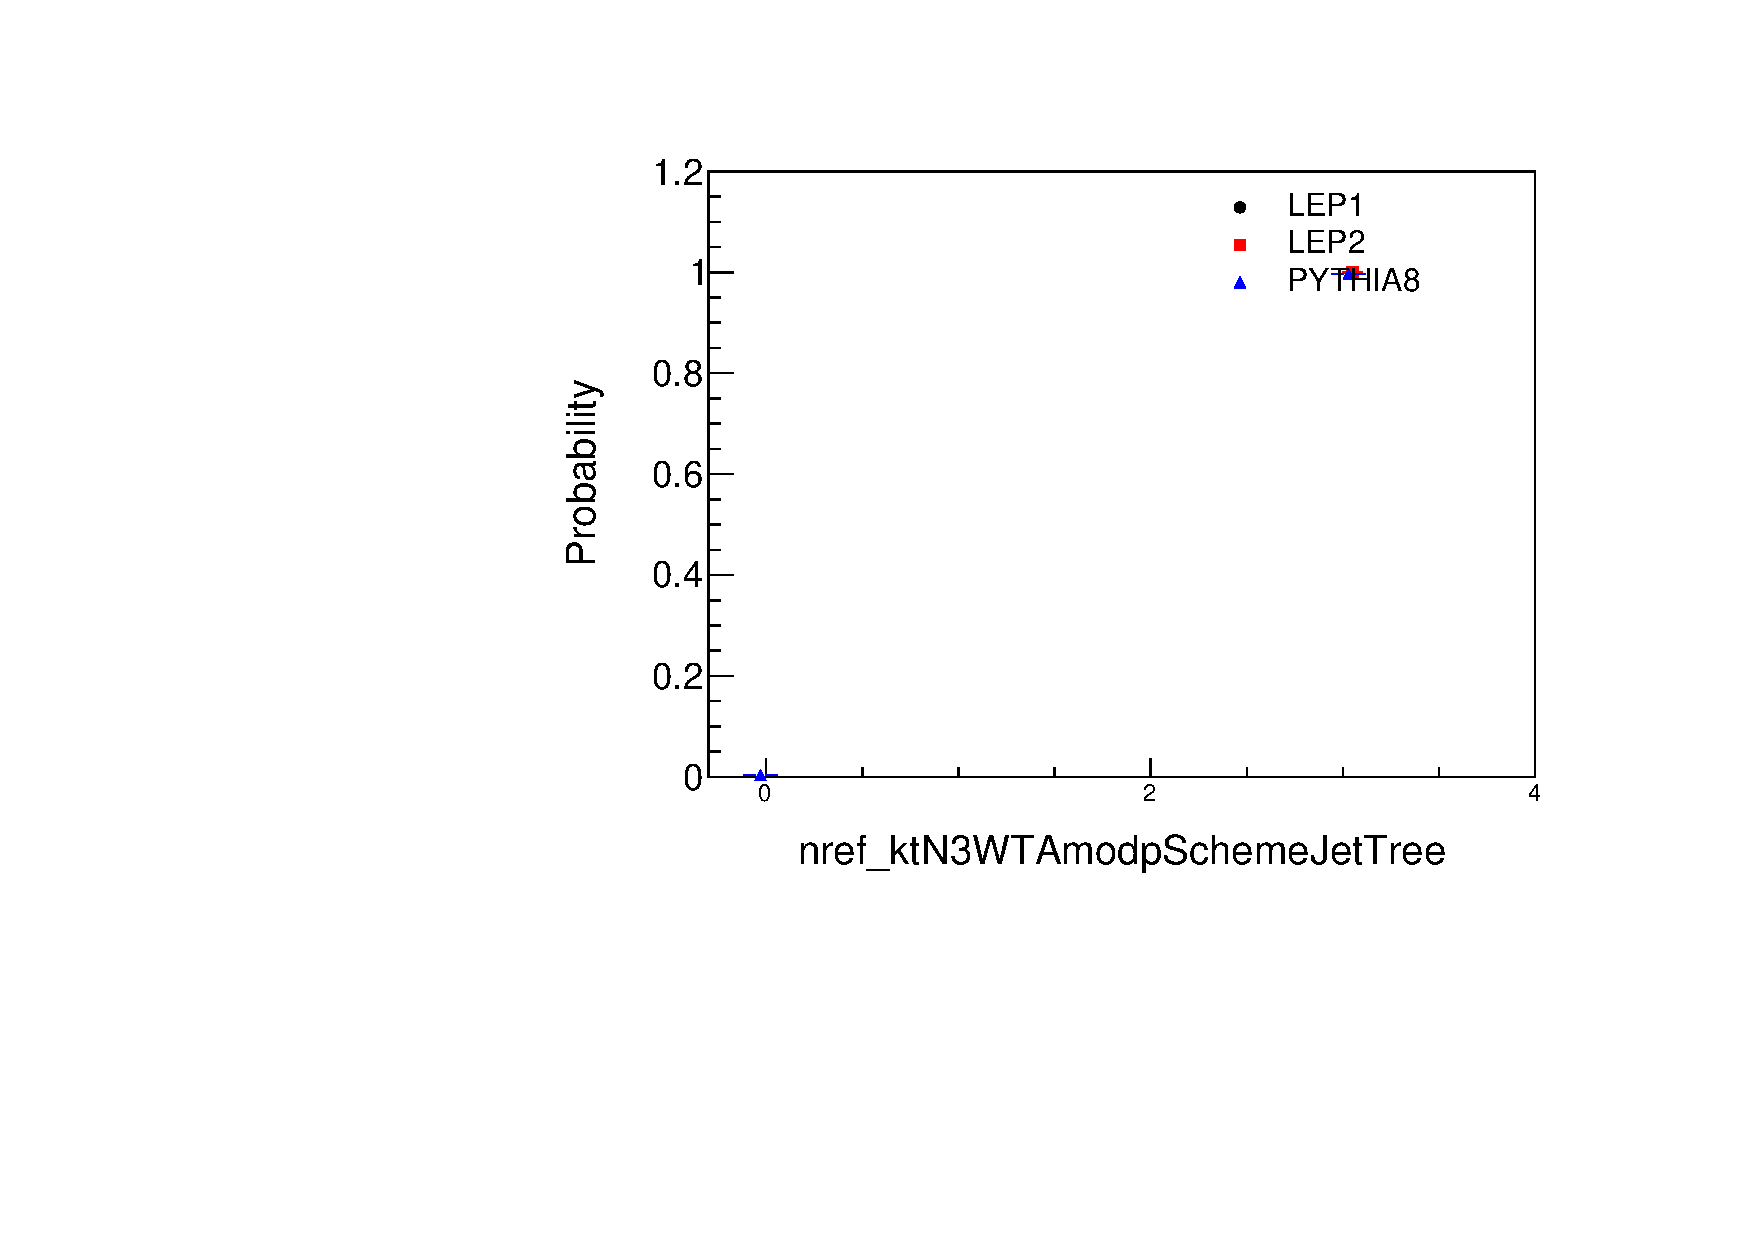
\includegraphics[width=.25\textwidth]{images/DQC/NoCut/nref_ktN3WTAmodpSchemeJetTree.pdf}}\hfill
\caption{Raw Data: LEP1, LEP2, Pythia8 no cuts. Jet nref distributions. Top row: anti-$k_t$, left to right: $R=0.4$, $E$ scheme; $R=0.8$, $E$ scheme; $R=0.4$, WTA mod p scheme; $R=0.8$, WTA mod p scheme. Bottom row: $k_t$, left to right: $N=2$, $E$ scheme; $N=3$, $E$ scheme; $N=2$, WTA mod p scheme; $N=3$; WTA mod p scheme.}  
\end{figure}

\begin{figure}[H]
\centering
\subfloat{\label{sfig:a}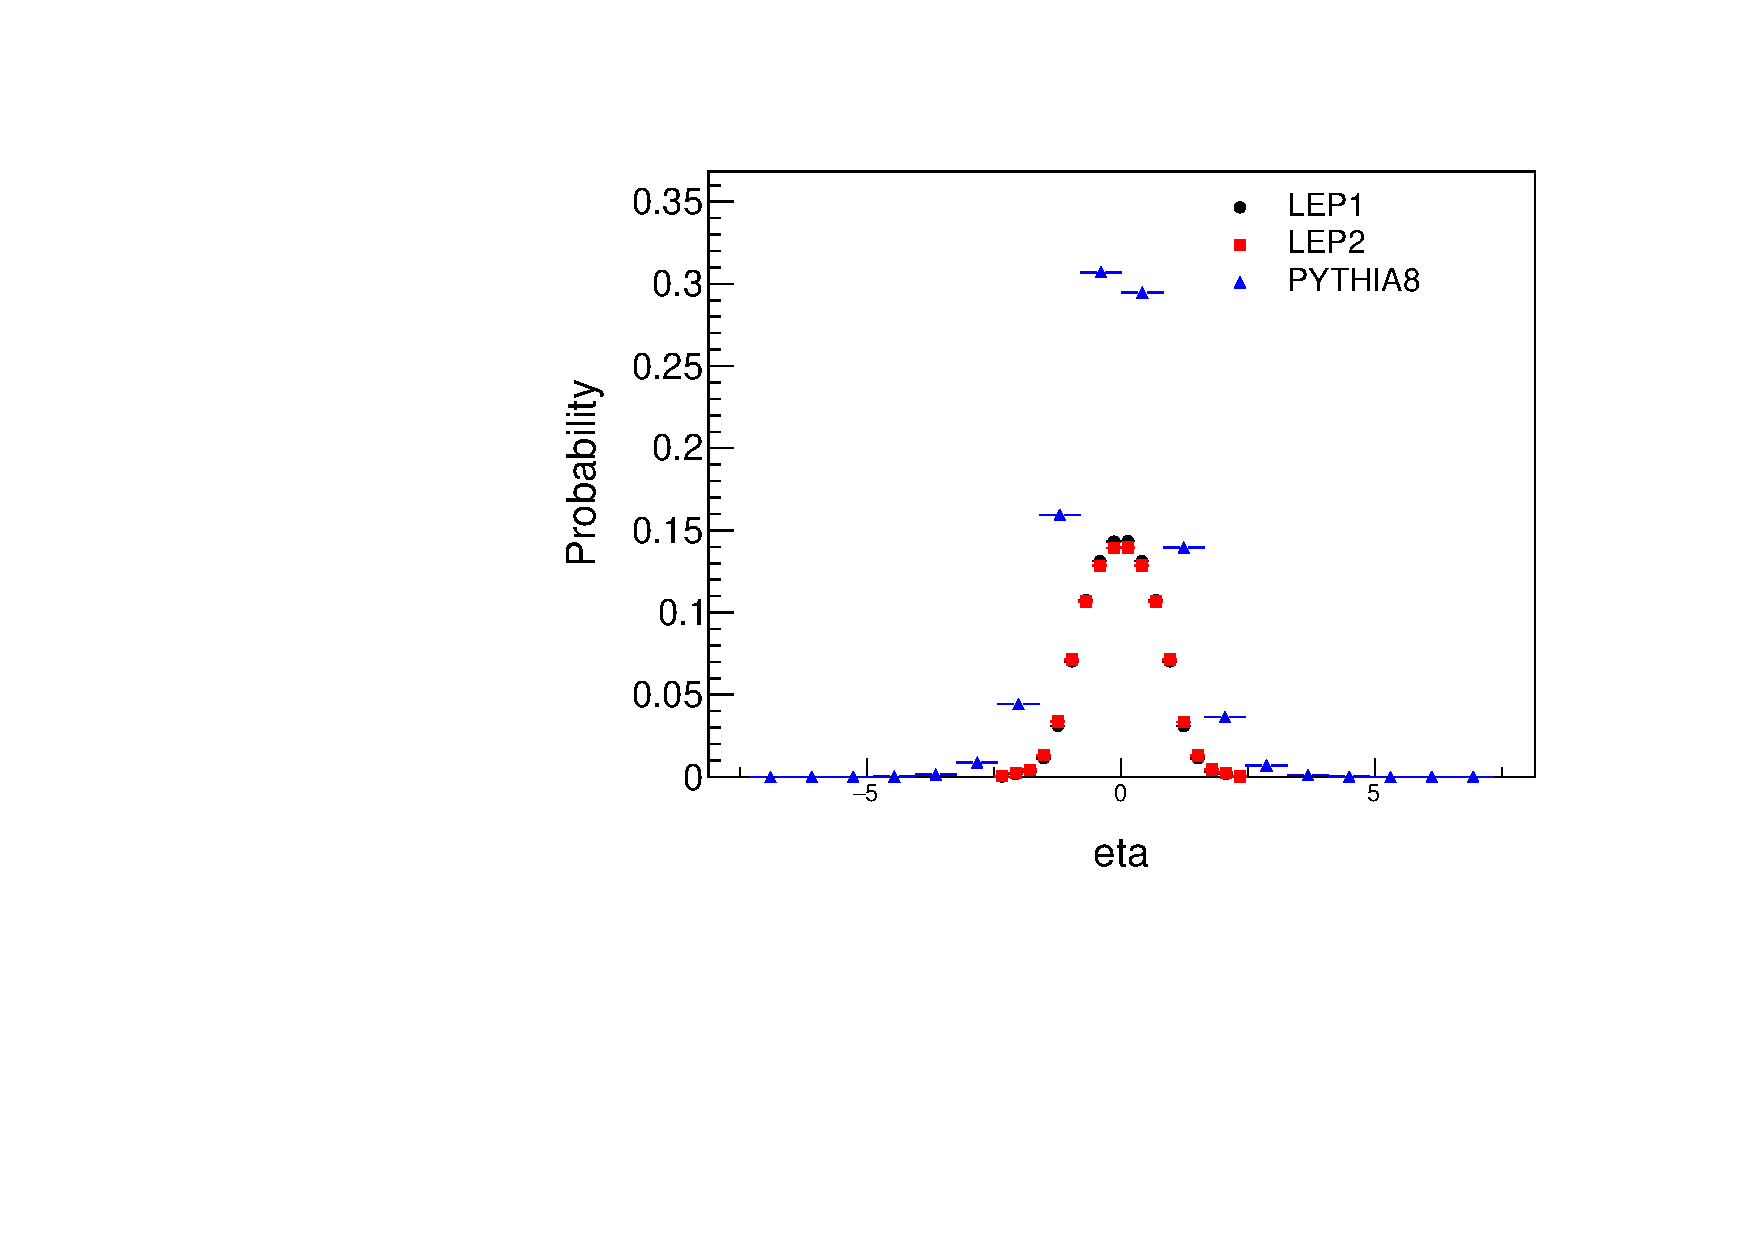
\includegraphics[width=.33\textwidth]{images/DQC/NoCut/eta.pdf}}\hfill
\subfloat{\label{sfig:b}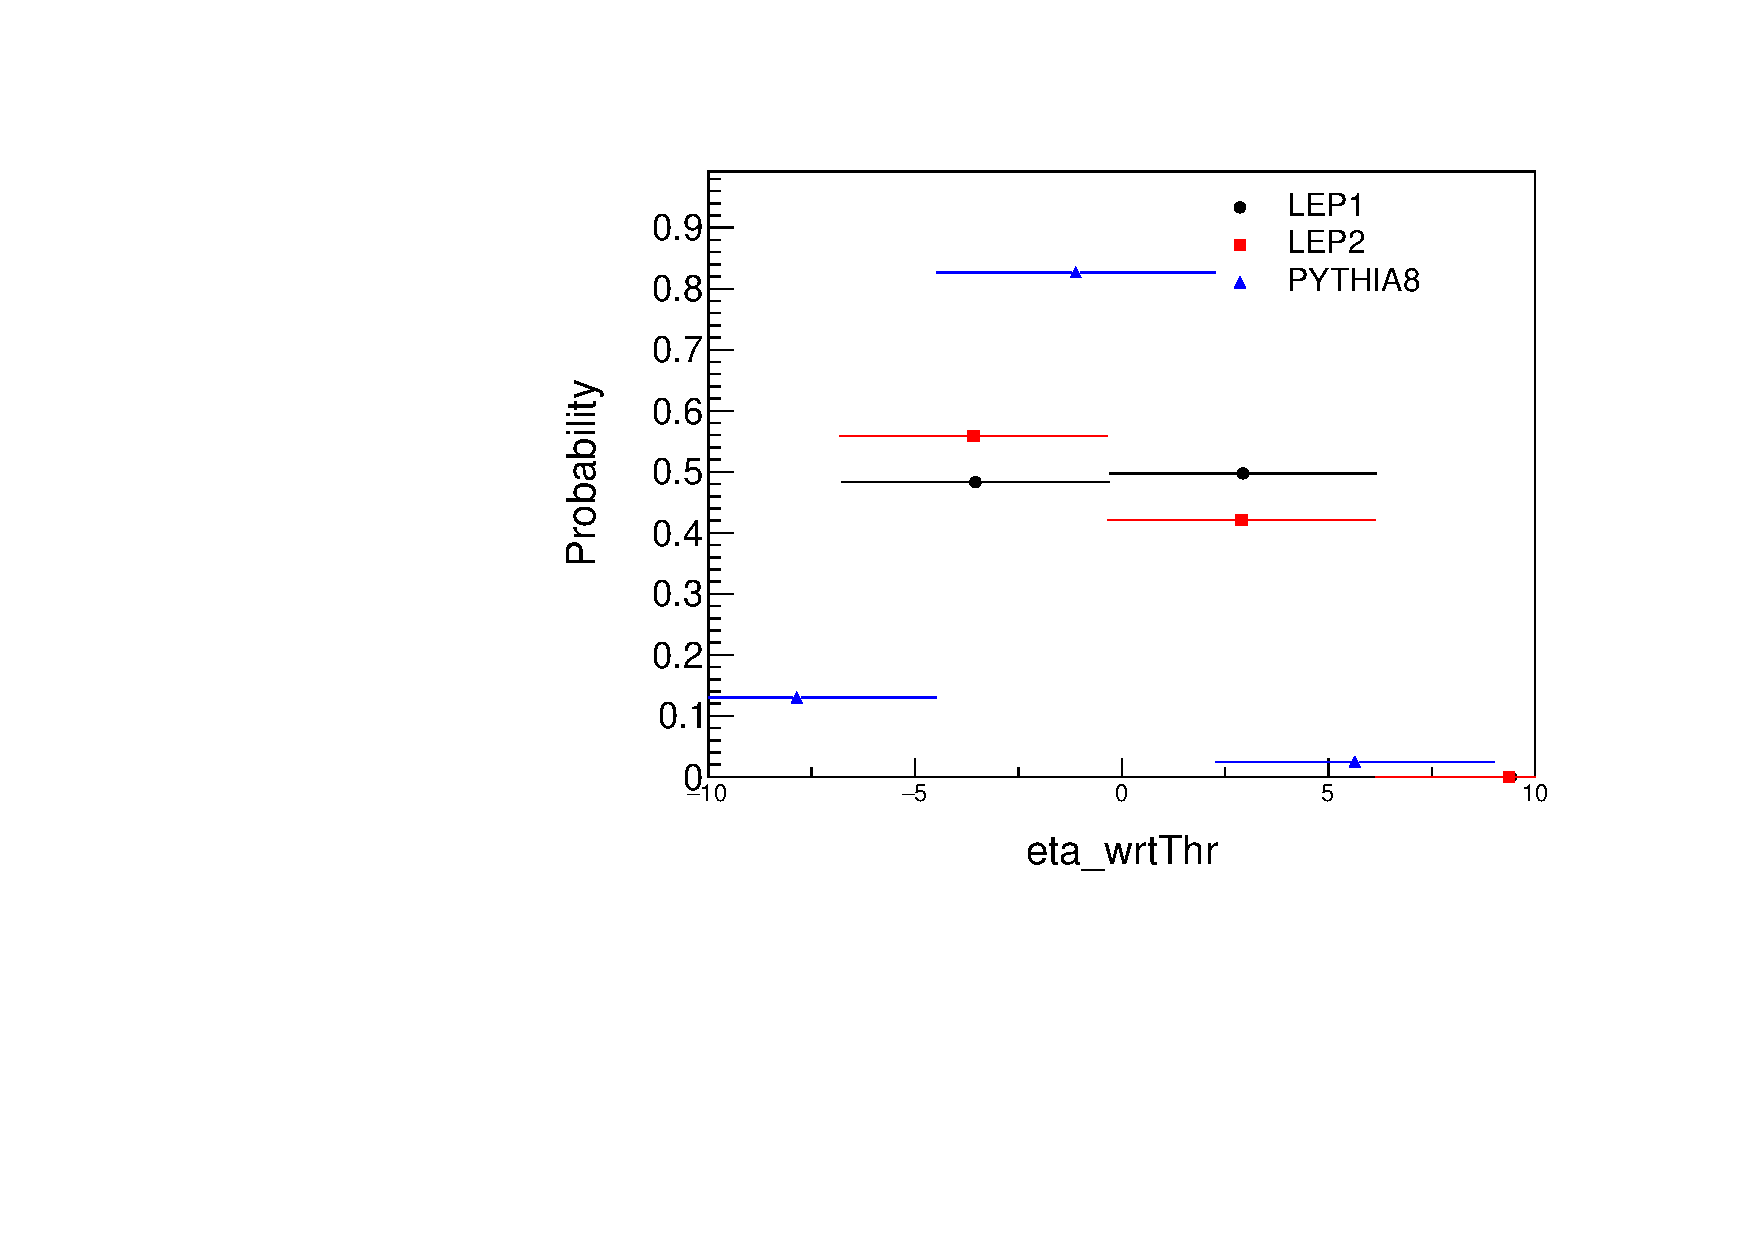
\includegraphics[width=.33\textwidth]{images/DQC/NoCut/eta_wrtThr.pdf}}\hfill
\subfloat{\label{sfig:c}\includegraphics[width=.33\textwidth]{images/DQC/NoCut/eta_wrtChThr.pdf}}\hfill
\caption{Raw Data: LEP1, LEP2, Pythia8 no cuts. $\eta$ distributions. Left to right: $\eta$; $\eta$ with respect to thrust axis; $\eta$ with respect to charged thrust axis.}
\end{figure}

\begin{figure}[H]
\centering
\subfloat{\label{sfig:a}\includegraphics[width=.33\textwidth]{images/DQC/NoCut/phi.pdf}}\hfill
\subfloat{\label{sfig:b}\includegraphics[width=.33\textwidth]{images/DQC/NoCut/phi_wrtThr.pdf}}\hfill
\subfloat{\label{sfig:c}\includegraphics[width=.33\textwidth]{images/DQC/NoCut/phi_wrtChThr.pdf}}\hfill
\caption{Raw Data: LEP1, LEP2, Pythia8 no cuts. $\phi$ distributions. Left to right: $\phi$; $\phi$ with respect to thrust axis; $\phi$ with respect to charged thrust axis.}
\end{figure}

\begin{figure}[H]
\centering
\subfloat{\label{sfig:a}\includegraphics[width=.33\textwidth]{images/DQC/NoCut/pt.pdf}}\hfill
\subfloat{\label{sfig:b}\includegraphics[width=.33\textwidth]{images/DQC/NoCut/pt_wrtThr.pdf}}\hfill
\subfloat{\label{sfig:c}\includegraphics[width=.33\textwidth]{images/DQC/NoCut/pt_wrtChThr.pdf}}\hfill
\caption{Raw Data: LEP1, LEP2, Pythia8 no cuts. $p_t$ distributions. Left to right: $p_t$; $p_t$ with respect to thrust axis; $p_t$ with respect to charged thrust axis.}
\end{figure}

\begin{figure}[H]
\centering
\subfloat{\label{sfig:a}\includegraphics[width=.33\textwidth]{images/DQC/NoCut/theta.pdf}}\hfill
\subfloat{\label{sfig:b}\includegraphics[width=.33\textwidth]{images/DQC/NoCut/theta_wrtThr.pdf}}\hfill
\subfloat{\label{sfig:c}\includegraphics[width=.33\textwidth]{images/DQC/NoCut/theta_wrtChThr.pdf}}\hfill
\caption{Raw Data: LEP1, LEP2, Pythia8 no cuts. $\theta$ distributions. Left to right: $\theta$; $\theta$ with respect to thrust axis; $\theta$ with respect to charged thrust axis.}
\end{figure}

\begin{figure}[H]
\centering
\subfloat{\label{sfig:a}\includegraphics[width=.25\textwidth]{images/DQC/NoCut/px.pdf}}\hfill
\subfloat{\label{sfig:b}\includegraphics[width=.25\textwidth]{images/DQC/NoCut/py.pdf}}\hfill
\subfloat{\label{sfig:c}\includegraphics[width=.25\textwidth]{images/DQC/NoCut/pz.pdf}}\hfill
\subfloat{\label{sfig:a}\includegraphics[width=.25\textwidth]{images/DQC/NoCut/pmag.pdf}}\hfill
\caption{Raw Data: LEP1, LEP2, Pythia8 no cuts. $p_x$, $p_y$, $p_z$, and $|\vec{p}|$ distributions.}
\end{figure}

\begin{figure}[H]
\centering
\subfloat{\label{sfig:a}\includegraphics[width=.25\textwidth]{images/DQC/NoCut/missP.pdf}}\hfill
\subfloat{\label{sfig:b}\includegraphics[width=.25\textwidth]{images/DQC/NoCut/missPt.pdf}}\hfill
\subfloat{\label{sfig:c}\includegraphics[width=.25\textwidth]{images/DQC/NoCut/missTheta.pdf}}\hfill
\subfloat{\label{sfig:d}\includegraphics[width=.25\textwidth]{images/DQC/NoCut/missPhi.pdf}}\hfill %row end
\subfloat{\label{sfig:e}\includegraphics[width=.25\textwidth]{images/DQC/NoCut/missChargedP.pdf}}\hfill
\subfloat{\label{sfig:f}\includegraphics[width=.25\textwidth]{images/DQC/NoCut/missChargedPt.pdf}}\hfill
\subfloat{\label{sfig:g}\includegraphics[width=.25\textwidth]{images/DQC/NoCut/missChargedTheta.pdf}}\hfill
\subfloat{\label{sfig:h}\includegraphics[width=.25\textwidth]{images/DQC/NoCut/missChargedPhi.pdf}}\hfill
\caption{Raw Data: LEP1, LEP2, Pythia8 no cuts. missing quantities distribution. Left to right: missing $P$; missing $p_t$; missing $\theta$; missing $\phi$. Top to bottom: All; charged.}  
\end{figure}

\begin{figure}[H]
\centering
\subfloat{\label{sfig:a}\includegraphics[width=.33\textwidth]{images/DQC/NoCut/charge.pdf}}\hfill
\subfloat{\label{sfig:b}\includegraphics[width=.33\textwidth]{images/DQC/NoCut/d0.pdf}}\hfill
\subfloat{\label{sfig:c}\includegraphics[width=.33\textwidth]{images/DQC/NoCut/Energy.pdf}}\hfill %row end
\subfloat{\label{sfig:d}\includegraphics[width=.33\textwidth]{images/DQC/NoCut/mass.pdf}}\hfill
\subfloat{\label{sfig:e}\includegraphics[width=.33\textwidth]{images/DQC/NoCut/nTrk.pdf}}\hfill
\subfloat{\label{sfig:f}\includegraphics[width=.33\textwidth]{images/DQC/NoCut/pwflag.pdf}}\hfill
\caption{Left to right: Top row: Raw Data: LEP1, LEP2, Pythia8 no cuts. charge, $d_0$, and energy distributions. Bottom row: NoCut mass, particle multiplicity, and pwflag distributions.}
\end{figure}

\begin{figure}[H]
\centering
\subfloat{\label{sfig:a}\includegraphics[width=.5\textwidth]{images/DQC/NoCut/bx.pdf}}\hfill
\subfloat{\label{sfig:b}\includegraphics[width=.5\textwidth]{images/DQC/NoCut/by.pdf}}\hfill %row end
\subfloat{\label{sfig:c}\includegraphics[width=.5\textwidth]{images/DQC/NoCut/ebx.pdf}}\hfill
\subfloat{\label{sfig:d}\includegraphics[width=.5\textwidth]{images/DQC/NoCut/eby.pdf}}\hfill
\caption{Top row: Raw Data: LEP1, LEP2, Pythia8 no cuts. beamspot $x$ and $y$. Bottom row: Error in beamspot $x$ and $y$.}
\end{figure}

\begin{figure}[H]
\centering
\subfloat{\label{sfig:a}\includegraphics[width=.5\textwidth]{images/DQC/NoCut/Thrust.pdf}}\hfill
\subfloat{\label{sfig:b}\includegraphics[width=.5\textwidth]{images/DQC/NoCut/Thrust_charged.pdf}}\hfill %row end
\caption{Left: Raw Data: LEP1, LEP2, Pythia8 no cuts. thrust distribution. Right: Raw Data: LEP1, LEP2, Pythia8 no cuts. charged thrust distribution.}
\end{figure}

\begin{figure}[H]
\centering
\subfloat{\label{sfig:a}\includegraphics[width=.33\textwidth]{images/DQC/NoCut/nChargedHadrons.pdf}}\hfill
\subfloat{\label{sfig:b}\includegraphics[width=.33\textwidth]{images/DQC/NoCut/nChargedHadrons_GT0p4.pdf}}\hfill
\subfloat{\label{sfig:c}\includegraphics[width=.33\textwidth]{images/DQC/NoCut/nChargedHadrons_GT0p4Thrust.pdf}}\hfill
\caption{Raw Data: LEP1, LEP2, Pythia8 no cuts. charged hadron multiplicity distributions. Left to right: charged hadron multiplicity; charged hadron multiplicity (GT0p4); charged hadron multiplicity (GT0p4Thrust).}
\end{figure}

\begin{figure}[H]
\centering
\subfloat{\label{sfig:a}\includegraphics[width=.33\textwidth]{images/DQC/NoCut/z0.pdf}}\hfill
\subfloat{\label{sfig:b}\includegraphics[width=.33\textwidth]{images/DQC/NoCut/ntpc.pdf}}\hfill %row end
\subfloat{\label{sfig:c}\includegraphics[width=.33\textwidth]{images/DQC/NoCut/rap.pdf}}\hfill %row end
\caption{Left: Raw Data: LEP1, LEP2, Pythia8 no cuts. $z_0$ distribution. Center: Raw Data: LEP1, LEP2, Pythia8 no cuts. TPC hits distribution. Right: NoCut rapidity distribution.}
\end{figure}

